% !TeX program = xelatex
\documentclass[10pt,a4paper]{ctexart} % 设置文章类型，正文字号与纸张大小

% 页面与正文常用宏包
\usepackage[margin=2cm]{geometry} % 设置页面四周页边距
\usepackage{graphicx}             % 插入图片
\usepackage{amsmath}              % 提供cases、aligned等数学公式环境
\usepackage{amssymb}              % 提供\therefore等扩展数学符号
\usepackage{booktabs}             % 提供\toprule、\midrule、\bottomrule三线表命令
\usepackage{float}                % 提供[H]固定图片、表格位置
\usepackage{subcaption}           % 提供subfigure子图环境及子图标题
\usepackage{wrapfig}              % 提供wrapfigure图文环绕环境
\usepackage{fancyhdr}             % 自定义页眉和页脚
\usepackage{hyperref}             % 生成超链接

% 页眉页脚
\pagestyle{fancy}                  % 启用fancyhdr定义的页面样式
\fancyhf{}                         % 清空默认页眉和页脚
\fancyfoot[C]{\thepage}            % 在页脚中央显示页码
\renewcommand{\headrulewidth}{0pt} % 隐藏页眉横线
\renewcommand{\footrulewidth}{0pt} % 隐藏页脚横线

% 超链接
\hypersetup{
  colorlinks=true,                % 使用彩色文字链接，而非带边框的链接
  linkcolor=red,                 % 目录、公式及图表交叉引用的颜色
  filecolor=cyan,                 % 本地文件链接的颜色
  urlcolor=blue,                  % 网址链接的颜色
  pdftitle={示波器的使用+组装整流器报告},     % 写入PDF文档属性的标题
  bookmarksnumbered=true          % PDF书签显示章节编号
}

% 定义字号命令
\newcommand{\chuhao}{\fontsize{42pt}{63pt}\selectfont}
\newcommand{\xiaochu}{\fontsize{36pt}{54pt}\selectfont}
\newcommand{\yihao}{\fontsize{26pt}{39pt}\selectfont}
\newcommand{\xiaoyi}{\fontsize{24pt}{36pt}\selectfont}
\newcommand{\erhao}{\fontsize{22pt}{33pt}\selectfont}
\newcommand{\xiaoer}{\fontsize{18pt}{27pt}\selectfont}
\newcommand{\sanhao}{\fontsize{16pt}{24pt}\selectfont}
\newcommand{\xiaosan}{\fontsize{15pt}{22.5pt}\selectfont}
\newcommand{\sihao}{\fontsize{14pt}{21pt}\selectfont}
\newcommand{\xiaosi}{\fontsize{12pt}{18pt}\selectfont}
\newcommand{\wuhao}{\fontsize{10.5pt}{15.75pt}\selectfont}
\newcommand{\xiaowu}{\fontsize{9pt}{13.5pt}\selectfont}

% 章节格式
\ctexset{
  section={
    format={\CJKfontspec[AutoFakeBold=2.5]{KaiTi}\sanhao\bfseries}, % 一级标题使用三号加粗楷体
    name={,、},                                                    % 在中文章节序号后添加顿号
    number=\chinese{section},                                      % 一级标题编号使用“一、二、三”形式
    aftername={}                                                   % 取消编号与标题文字之间的空格
  },
  subsection={
    format={\CJKfontspec[AutoFakeBold=2.5]{KaiTi}\sihao\bfseries}, % 二级标题使用四号加粗楷体                                               
  },
  subsubsection={
    format={\CJKfontspec[AutoFakeBold=2.5]{KaiTi}\xiaosi\bfseries}, % 三级标题使用小四加粗楷体
  }
}

\begin{document}

% 封面
\thispagestyle{fancy} % 封面保留底部居中的页码
\fancyfoot[C]{\thepage}
\begin{center}
  \CJKfontspec[AutoFakeBold=2.5]{KaiTi}\bfseries % 封面中文使用楷体并人工加粗，西文同时加粗
  \vspace{0.8cm}
  
\includegraphics[width=8.2cm]{figures/head.png}

  \vspace{0.2cm}
  \xiaochu 
    物理实验报告

  \vspace{3.5cm}
  \begin{minipage}{10.0cm}
    \sanhao
    \makebox[2.6cm][l]{实验名称：}
    \underline{\makebox[7.0cm][c]{示波器的使用+组装整流器}}\par\vspace{12pt}

    \makebox[2.6cm][l]{实验桌号：}
    \underline{\makebox[7.0cm][c]{18}}\par\vspace{12pt}

    \makebox[2.6cm][l]{指导教师：}
    \underline{\makebox[7.0cm][c]{居乐乐}}
  \end{minipage}

  \vspace{3.5cm}
  \begin{minipage}{10.0cm}
    \sihao
    \makebox[1.4cm][l]{班级：}
    \underline{\makebox[8.0cm][c]{}}\par\vspace{10pt}

    \makebox[1.4cm][l]{姓名：}
    \underline{\makebox[8.0cm][c]{IllusoryRain}}\par\vspace{10pt}

    \makebox[1.4cm][l]{学号：}
    \underline{\makebox[8.0cm][c]{}}
  \end{minipage}

  \vspace{2.0cm}
  \sihao
    实验日期：
    \underline{\makebox[0.7cm][c]{2026}}年
    \underline{\makebox[0.7cm][c]{10}}月
    \underline{\makebox[1.4cm][c]{10/14}}日
    星期\underline{\makebox[1.4cm][c]{六/三}}上午

  \vspace{0.7cm}
  \sihao 
    浙江大学物理实验教学中心
\end{center}

\newpage
\xiaosi\songti\mdseries % 后续正文统一使用小四不加粗的宋体

\section{预习报告（10分）}

  \subsection{实验综述（5分）}

    \subsubsection{示波器的使用}
    示波器的原理：示波器能将振荡信号以波形（正弦波、方波、锯齿波）显示在荧光屏上。
    它由示波管、放大器（包括X轴放大和Y轴放大）、扫描与触发同步系统和电源四个基本部分组成。

    李萨如图形是两个相互垂直的简谐振动叠加形成的轨迹。
    在X--Y模式下，将两路正弦信号分别接入CH1（X轴）和CH2（Y轴），
    当频率比为稳定的整数比时，可观察到稳定图形，并据此测量未知频率。

    信号频率和该轴上交点的数量成反比：
    \[
      \frac{f_y}{f_x}=\frac{T_x}{T_y}=\frac{N_x}{N_y},
      \qquad f_y=\frac{N_x}{N_y}f_x
    \]
    其中$N_x$、$N_y$分别为水平、竖直参考线的交点数。
    已知CH1（X轴）信号频率，即可测量CH2（Y轴）信号的频率；同频时也可测量相位差。

    \begin{figure}[H]
      \centering
      \begin{minipage}[c]{0.48\textwidth}
        \centering
        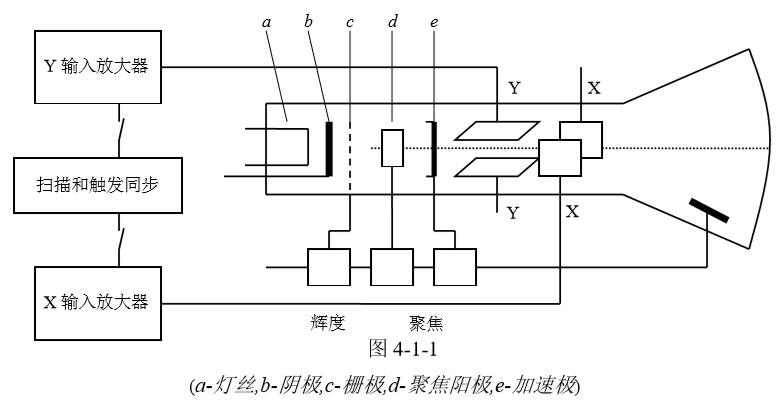
\includegraphics[width=0.95\textwidth]{figures/图1.png}
        \caption{示波器的基本结构}
      \end{minipage}
      \begin{minipage}[c]{0.48\textwidth}
        \centering
        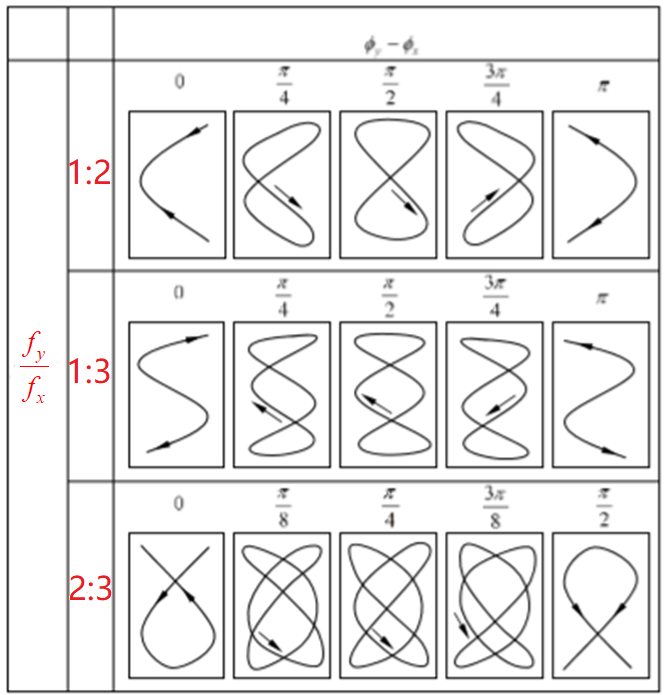
\includegraphics[width=0.8\textwidth]{figures/图2.png}
        \caption{不同频率比、相位差下的李萨如图形}
      \end{minipage}
    \end{figure}

    本实验包括以下三项内容：
    \begin{enumerate}
      \item 李萨如图测量未知频率：将已知频率信号接入X轴、未知信号接入Y轴，微调已知频率，
      待图形稳定后，记录交点数，按上述频率关系计算未知频率。

      \item 二极管导通电压测量：双通道同时观察二极管电路的输入、输出波形，
      用光标法或直读法读取电压，由输入、输出正峰值之差估算导通电压。
      
      \item RC电路相位差测量：双通道同时观察输入、输出波形，测量周期及对应特征点的时间差，
      根据时间差与周期的比值求出相位差，并判断输出信号的超前或滞后。
    \end{enumerate}

    \subsubsection{组装整流器}
    单相半波整流电路：
    \begin{itemize}
      \item 输出电压平均值：
      \[
        \overline{U}_0
        = \frac{1}{2\pi} \int_0^\pi
          \left(\sqrt{2}U_2\right)\sin(\omega t)\,\mathrm{d}(\omega t)
        = \frac{\sqrt{2}}{\pi}U_2
        = 0.45U_2
      \]

      \item 二极管承受最大反向电压：$\sqrt{2}U_2$

      \item 缺点：输出电压脉动大、效率低、二极管承受的反向电压大
    \end{itemize}

    \begin{figure}[H]
      \centering
      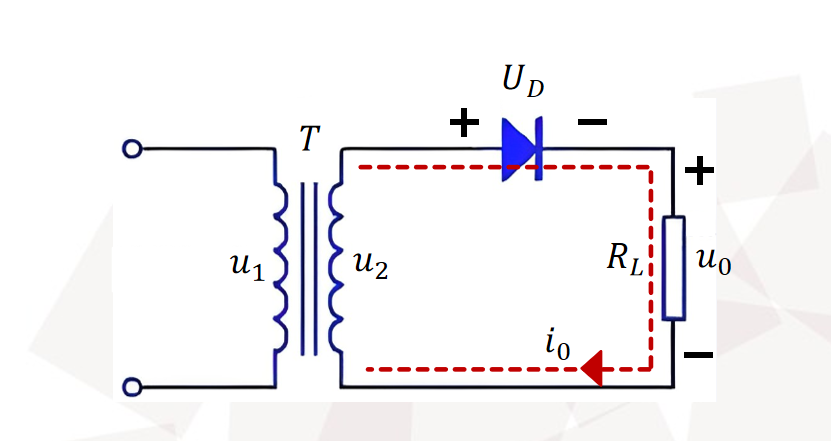
\includegraphics[width=0.4\textwidth]{figures/图3.png}
      \caption{单相半波整流电路}
    \end{figure}
    
    单相全波整流电路：
    \begin{itemize}
    \item 输出电压平均值：
    \[
        \overline{U}_0
        = \frac{1}{\pi}\int_{0}^{\pi}
        \left(\sqrt{2}U_2\right)\sin(\omega t)\,\mathrm{d}(\omega t)
        = \frac{2\sqrt{2}}{\pi}U_2
        = 0.9U_2
    \]

    \item 二极管承受最大反向电压：$2\sqrt{2}U_2$

    \item 缺点：电路结构复杂，需要中央抽头；二极管承受反向电压大
    \end{itemize}

    \begin{figure}[H]
      \centering
      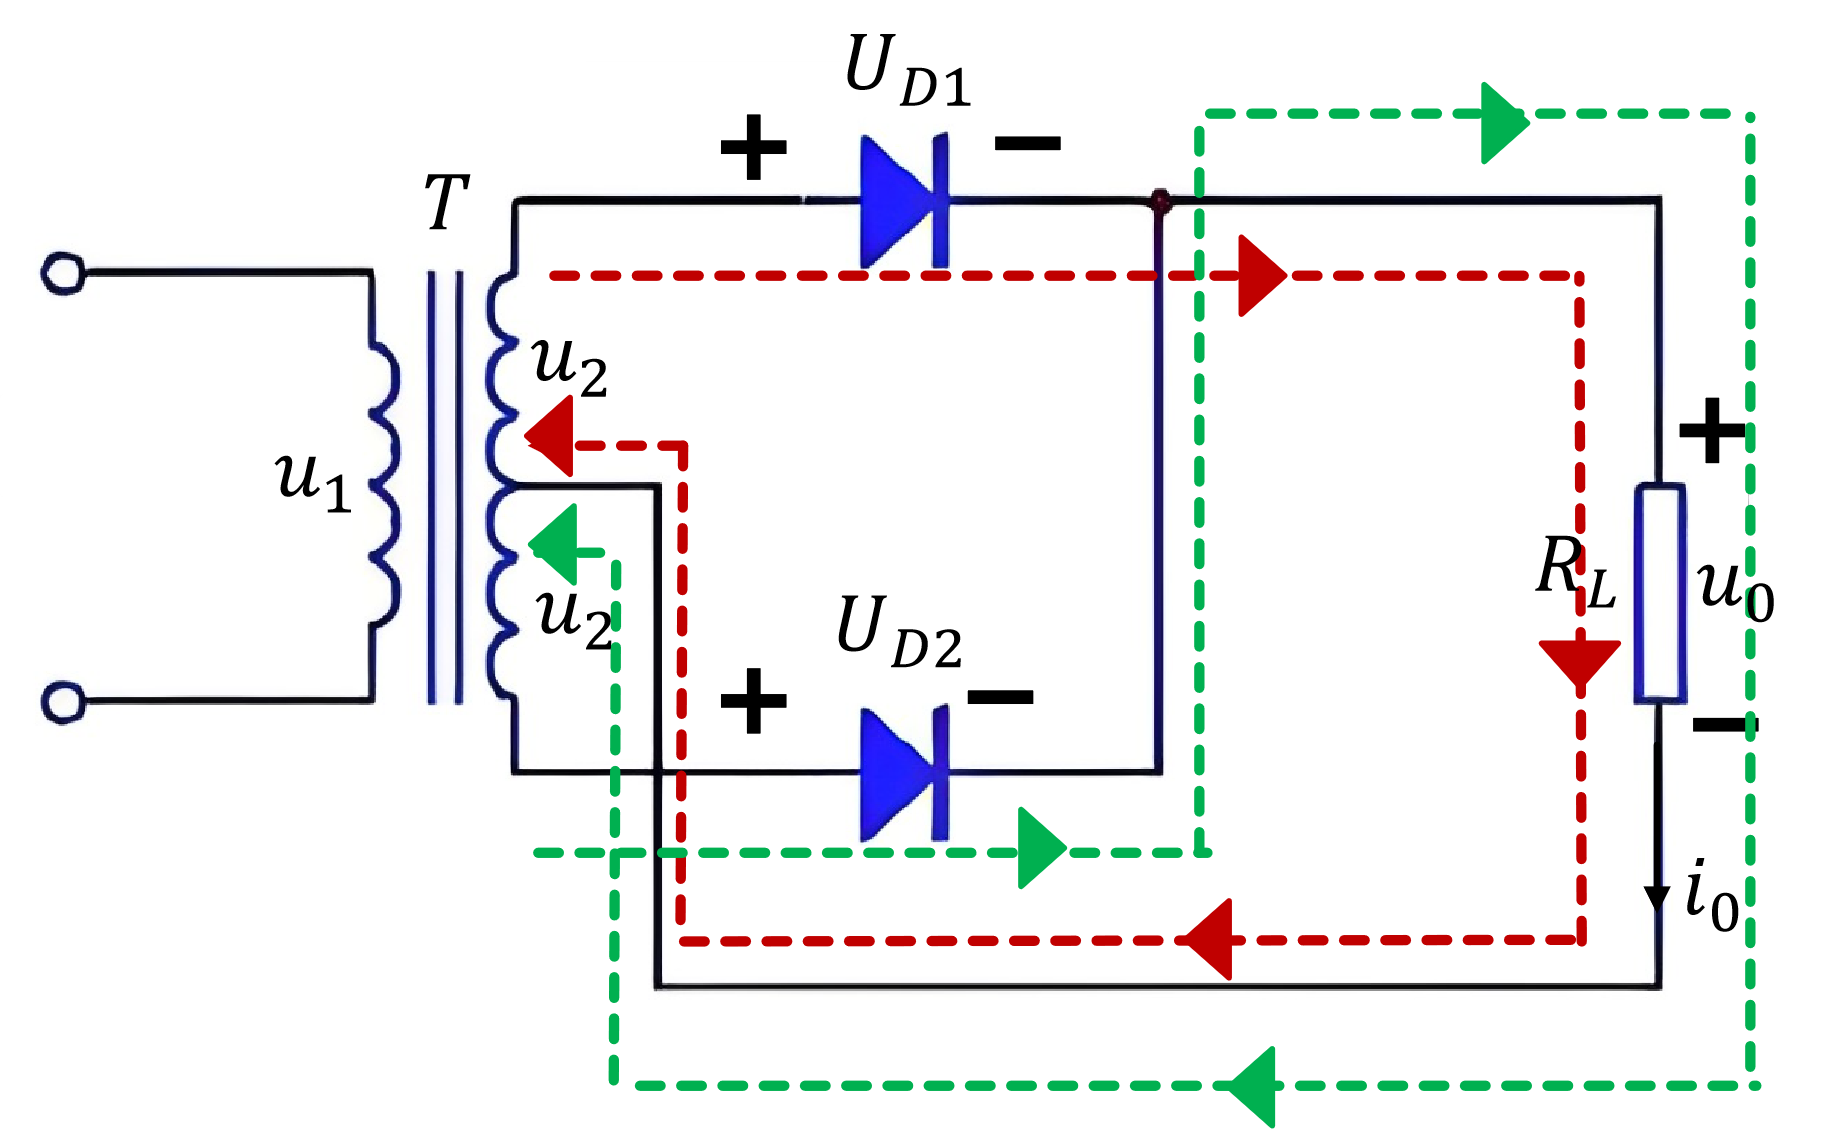
\includegraphics[width=0.4\textwidth]{figures/图4.png}
      \caption{单相全波整流电路}
    \end{figure}

    \newpage
    
    单相桥式整流电路：
    \begin{itemize}
    \item 输出电压平均值：
    \[
        \overline{U}_0
        = \frac{1}{\pi}\int_{0}^{\pi}
        \left(\sqrt{2}U_2\right)\sin(\omega t)\,\mathrm{d}(\omega t)
        = \frac{2\sqrt{2}}{\pi}U_2
        = 0.9U_2
    \]

    \item 二极管承受最大反向电压：$2\sqrt{2}U_2$

    \item 缺点：电路结构复杂，需要中央抽头；二极管承受反向电压大
    \end{itemize}

    \begin{figure}[H]
      \centering
      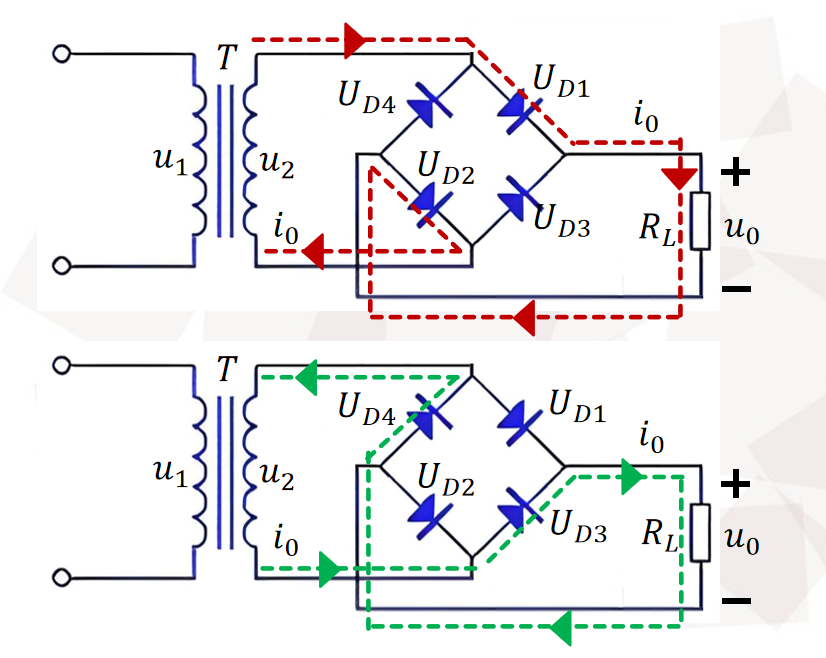
\includegraphics[width=0.4\textwidth]{figures/图5.png}
      \caption{单相桥式整流电路}
    \end{figure}

    滤波电路：
    \begin{figure}[H]
      \centering
      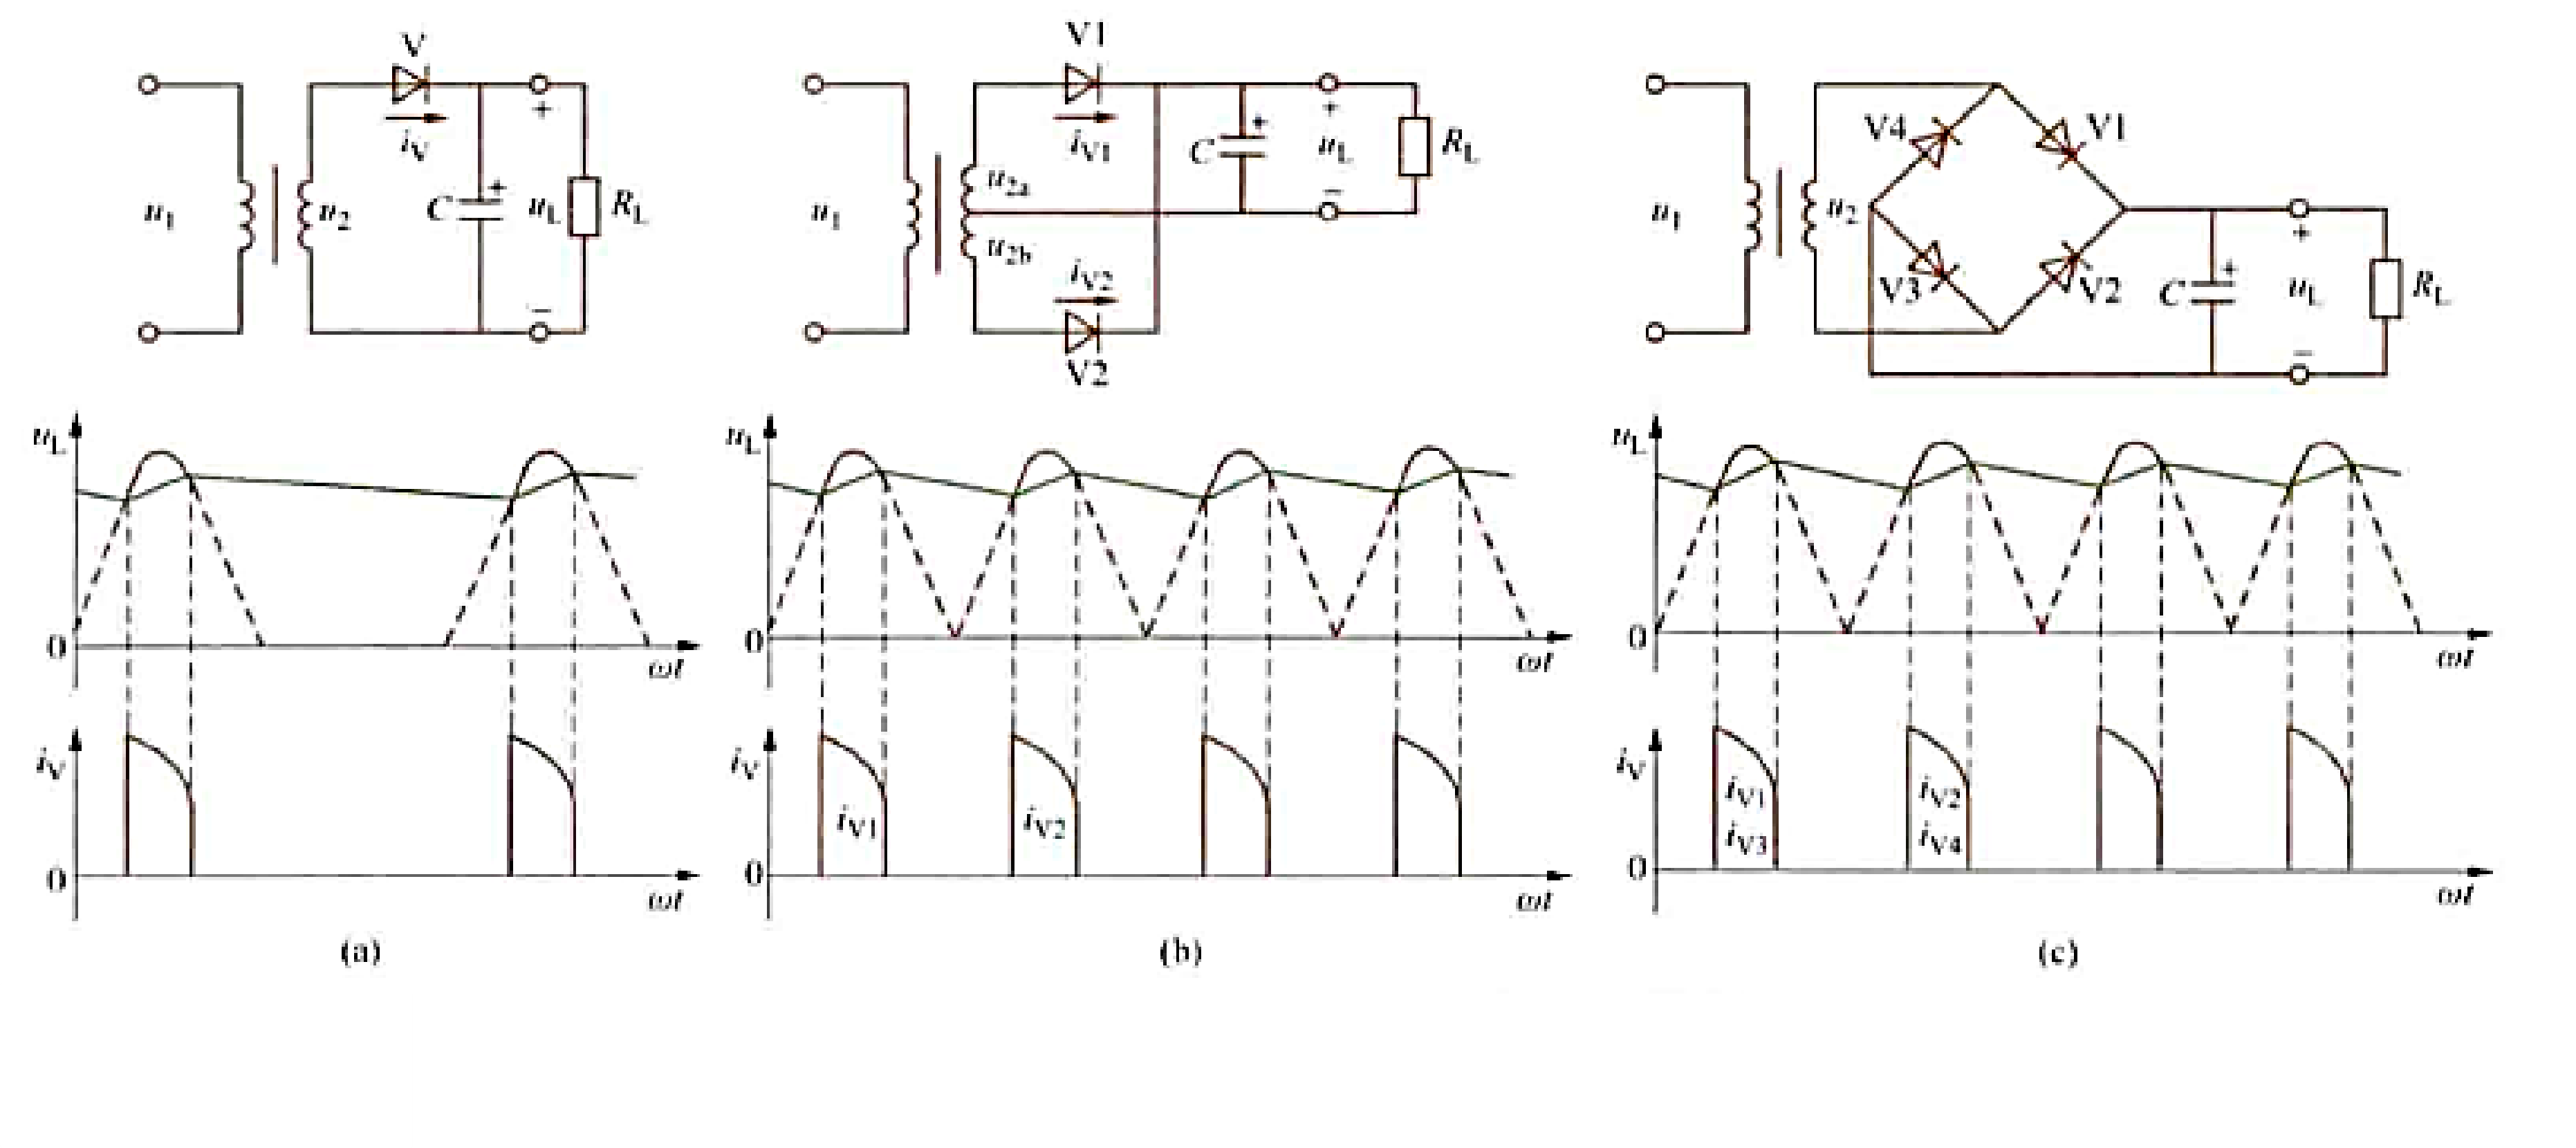
\includegraphics[width=0.6\textwidth]{figures/图6.png}
      \caption{滤波电路}
    \end{figure}

    实验包括以下两部分内容：

    组装整流电路：
    \begin{enumerate}
    \item 搭建单相半波整流电路、全波整流电路以及桥式整流电路。（示波器耦合模式：直流输入）观察输入波形、输出波形和二极管的反向电压波形，在表格中描绘波形。

    \item 使用示波器测量三种整流电路的以下参数，并在实验数据记录表格中记录：
      \begin{itemize}
        \item 输入信号的有效值$U_2$。
        \item 整流电路输出信号的有效值$U_0$和平均值$\overline{U}_0$。
        \item 整流电路中某个二极管的反向电压峰值$U_{\mathrm{Rmax}}$。
      \end{itemize}

    \item 计算无滤波器情况下，输出电压的平均值$\overline{U}_0$与公式所得的理论值之间的相对误差。
    \end{enumerate}
    
    观察RC滤波的效果：
    
    对于三种整流电路，分别添加47$\mu$F和470$\mu$F两种不同电容。观察RC滤波后的输出波形变化。
    比较不同电容值的滤波效果差异，并完成表格。
    
  \subsection{实验重点（3分）}
  
    \subsubsection{示波器的使用}
    \begin{enumerate}
      \item 从物理学角度了解示波器的结构和工作原理，了解示波器的扫描原理。
      \item 熟悉示波器面板旋钮的功能，掌握示波器的调节和使用方法。
      \item 学习用示波器观察信号波形，并测量其幅度大小、周期（或频率）、相位。
      \item 掌握用李萨如图形测量正弦信号频率的原理和方法。
    \end{enumerate}

    \subsubsection{组装整流器}
    \begin{enumerate}
      \item 了解整流电路与滤波电路的功能。
      \item 完成三种整流电路以及滤波电路的设计与组装。
      \item 熟悉掌握数字示波器的使用，了解一些常用电子元件的使用方法。
    \end{enumerate}

  \subsection{实验难点（2分）}

    \subsubsection{示波器的使用}
    \begin{enumerate}
      \item 调节时基与触发使波形稳定，正确判读李萨如图形的交点数与频率比。
      \item 准确读取输入、输出正峰值，利用其差值估算二极管导通电压。
      \item 测量RC电路输入、输出的周期和时间差，计算相位差并判断超前或滞后。
    \end{enumerate}

    \subsubsection{组装整流器}
    \begin{enumerate}
      \item 正确连接半波、全波和桥式整流电路，注意二极管方向及滤波电容极性。
      \item 区分有效值、平均值与峰值，准确测量整流电路各项电压参数。
      \item 比较两种电容的滤波效果，并计算无滤波时输出平均电压与理论值的相对误差。
    \end{enumerate}

\section{实验操作与原始数据（50分）}
% 填写自己的实验数据图

\section{结果与分析（30分）}

  \subsection{数据处理与结果（20分）}  
  
    \subsubsection{示波器的使用}
    实验一：二极管正向导通电压测量

    \begin{figure}[H]
      \centering
      \begin{minipage}[c]{0.4\textwidth}
        \centering
        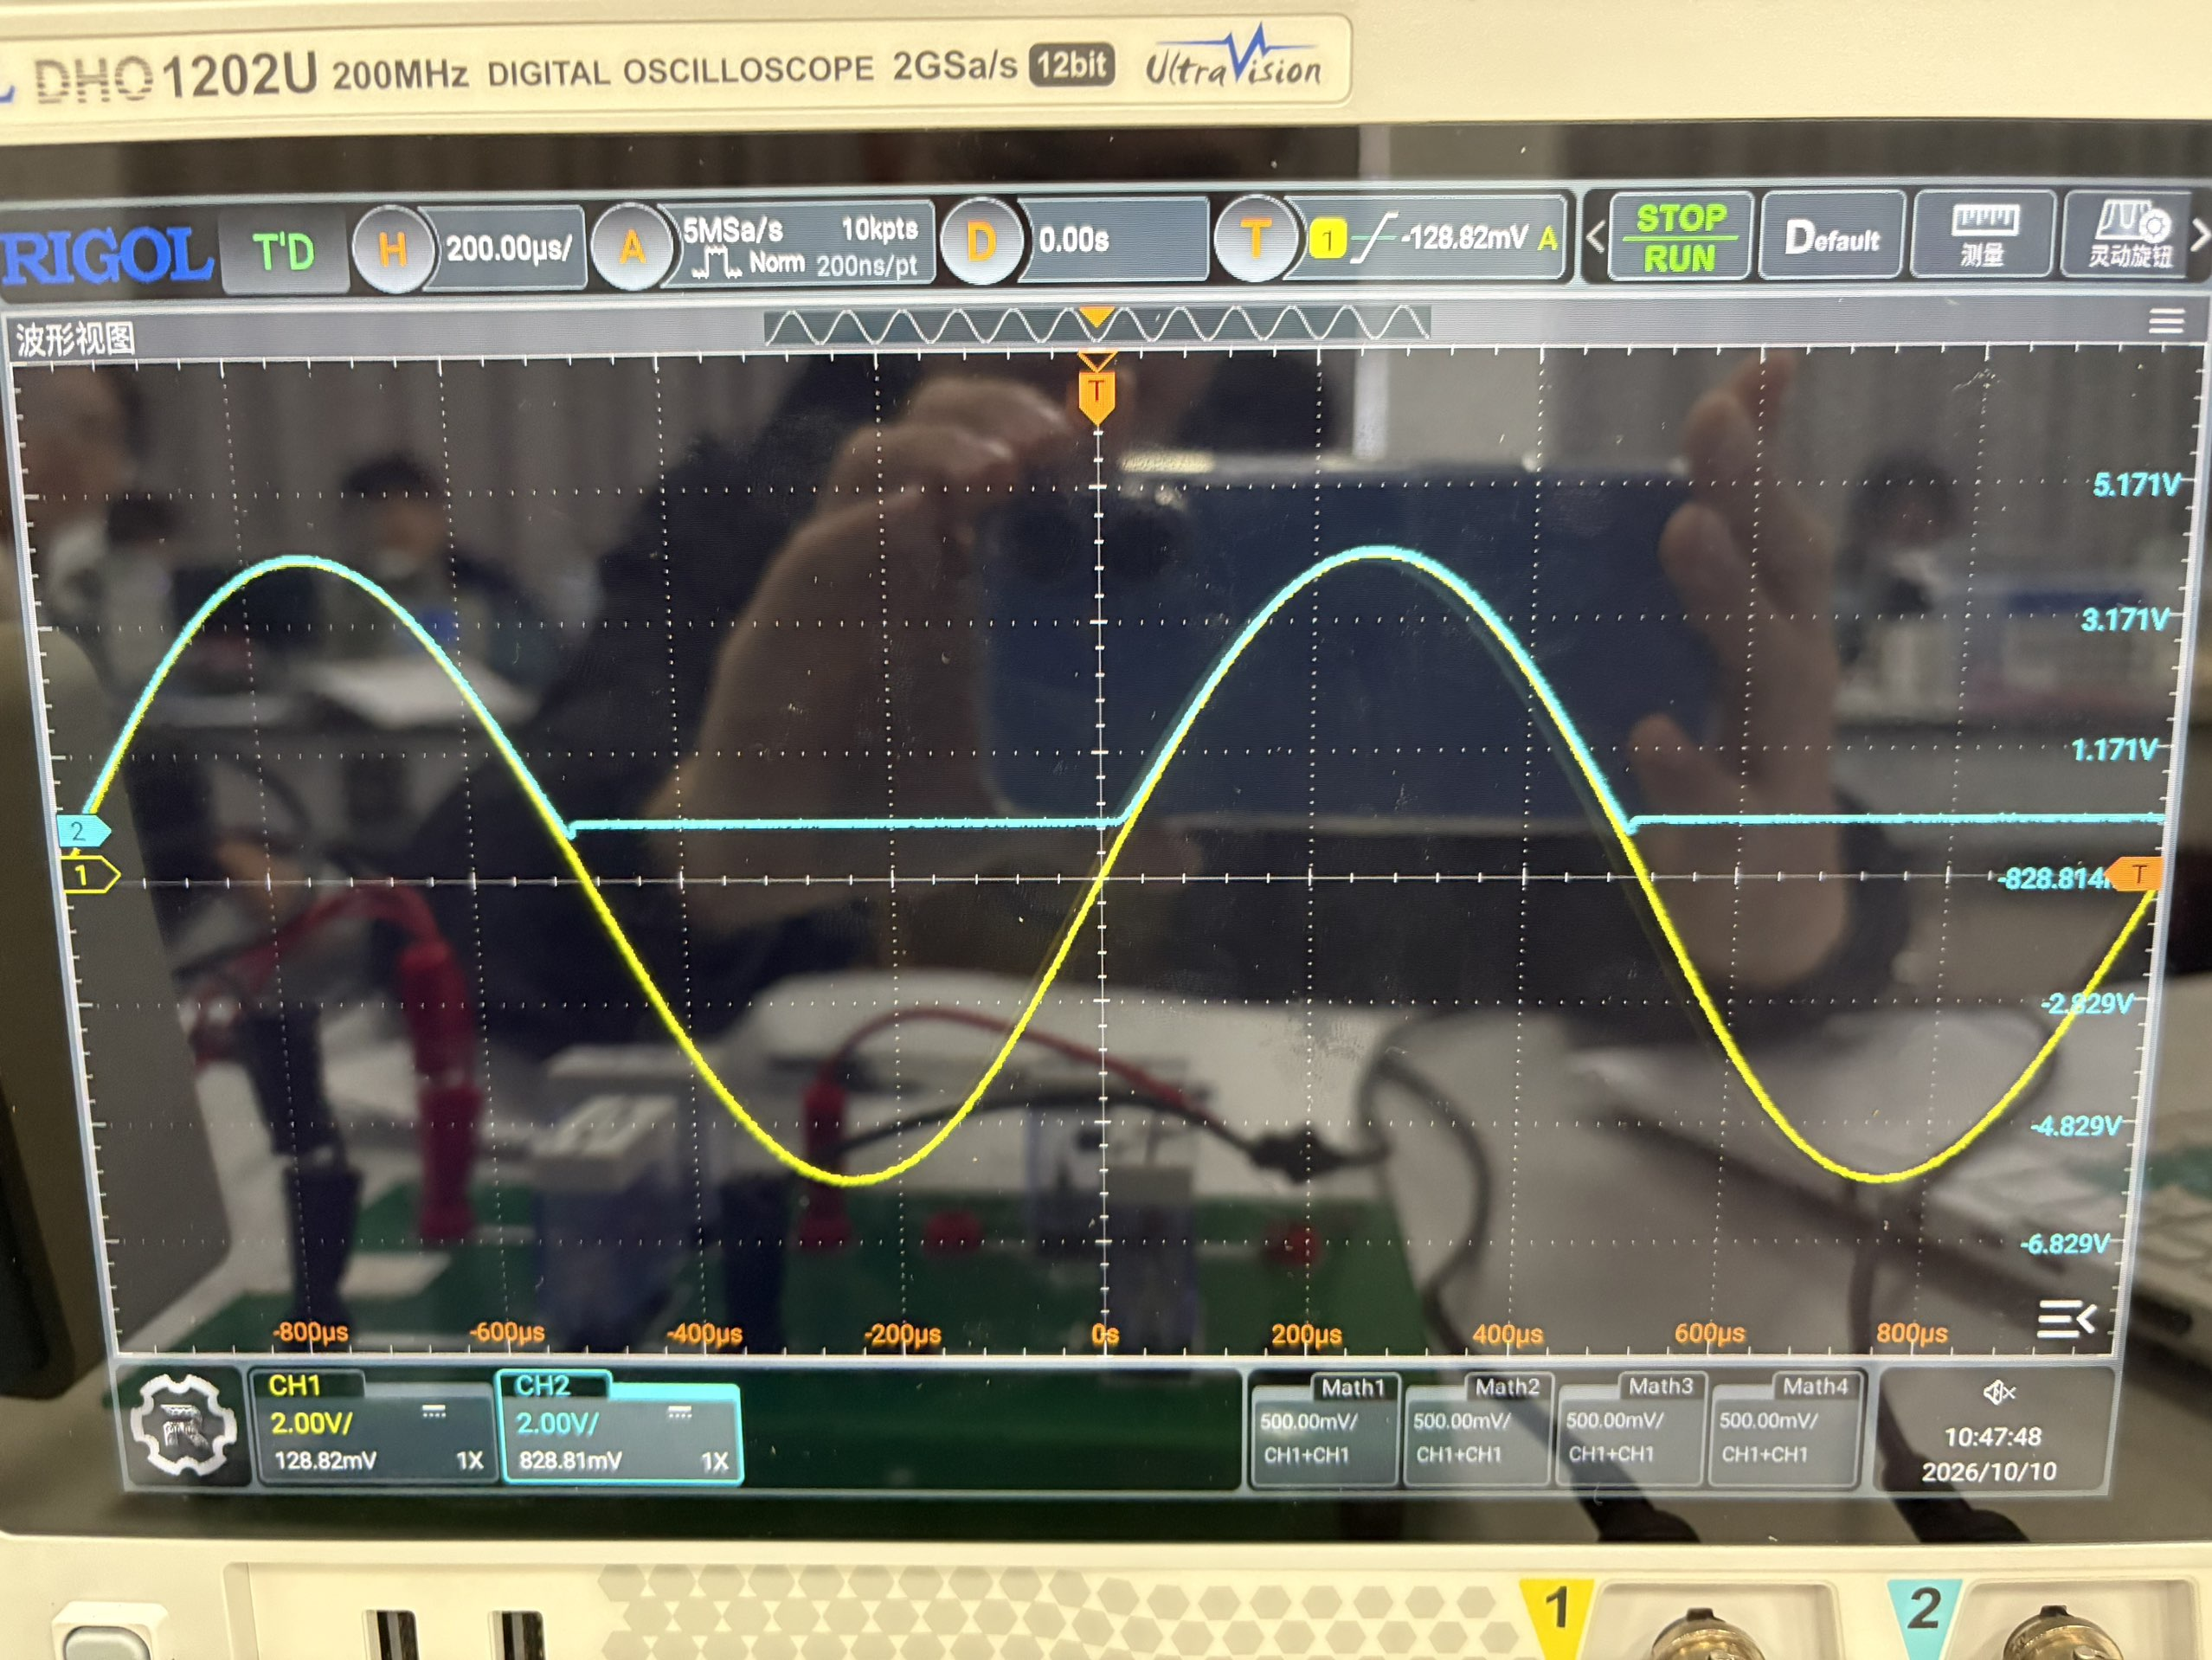
\includegraphics[width=0.8\textwidth]{figures/图9.png}
        \caption{二极管正向导通电压测量1}
      \end{minipage}
      \begin{minipage}[c]{0.4\textwidth}
        \centering
        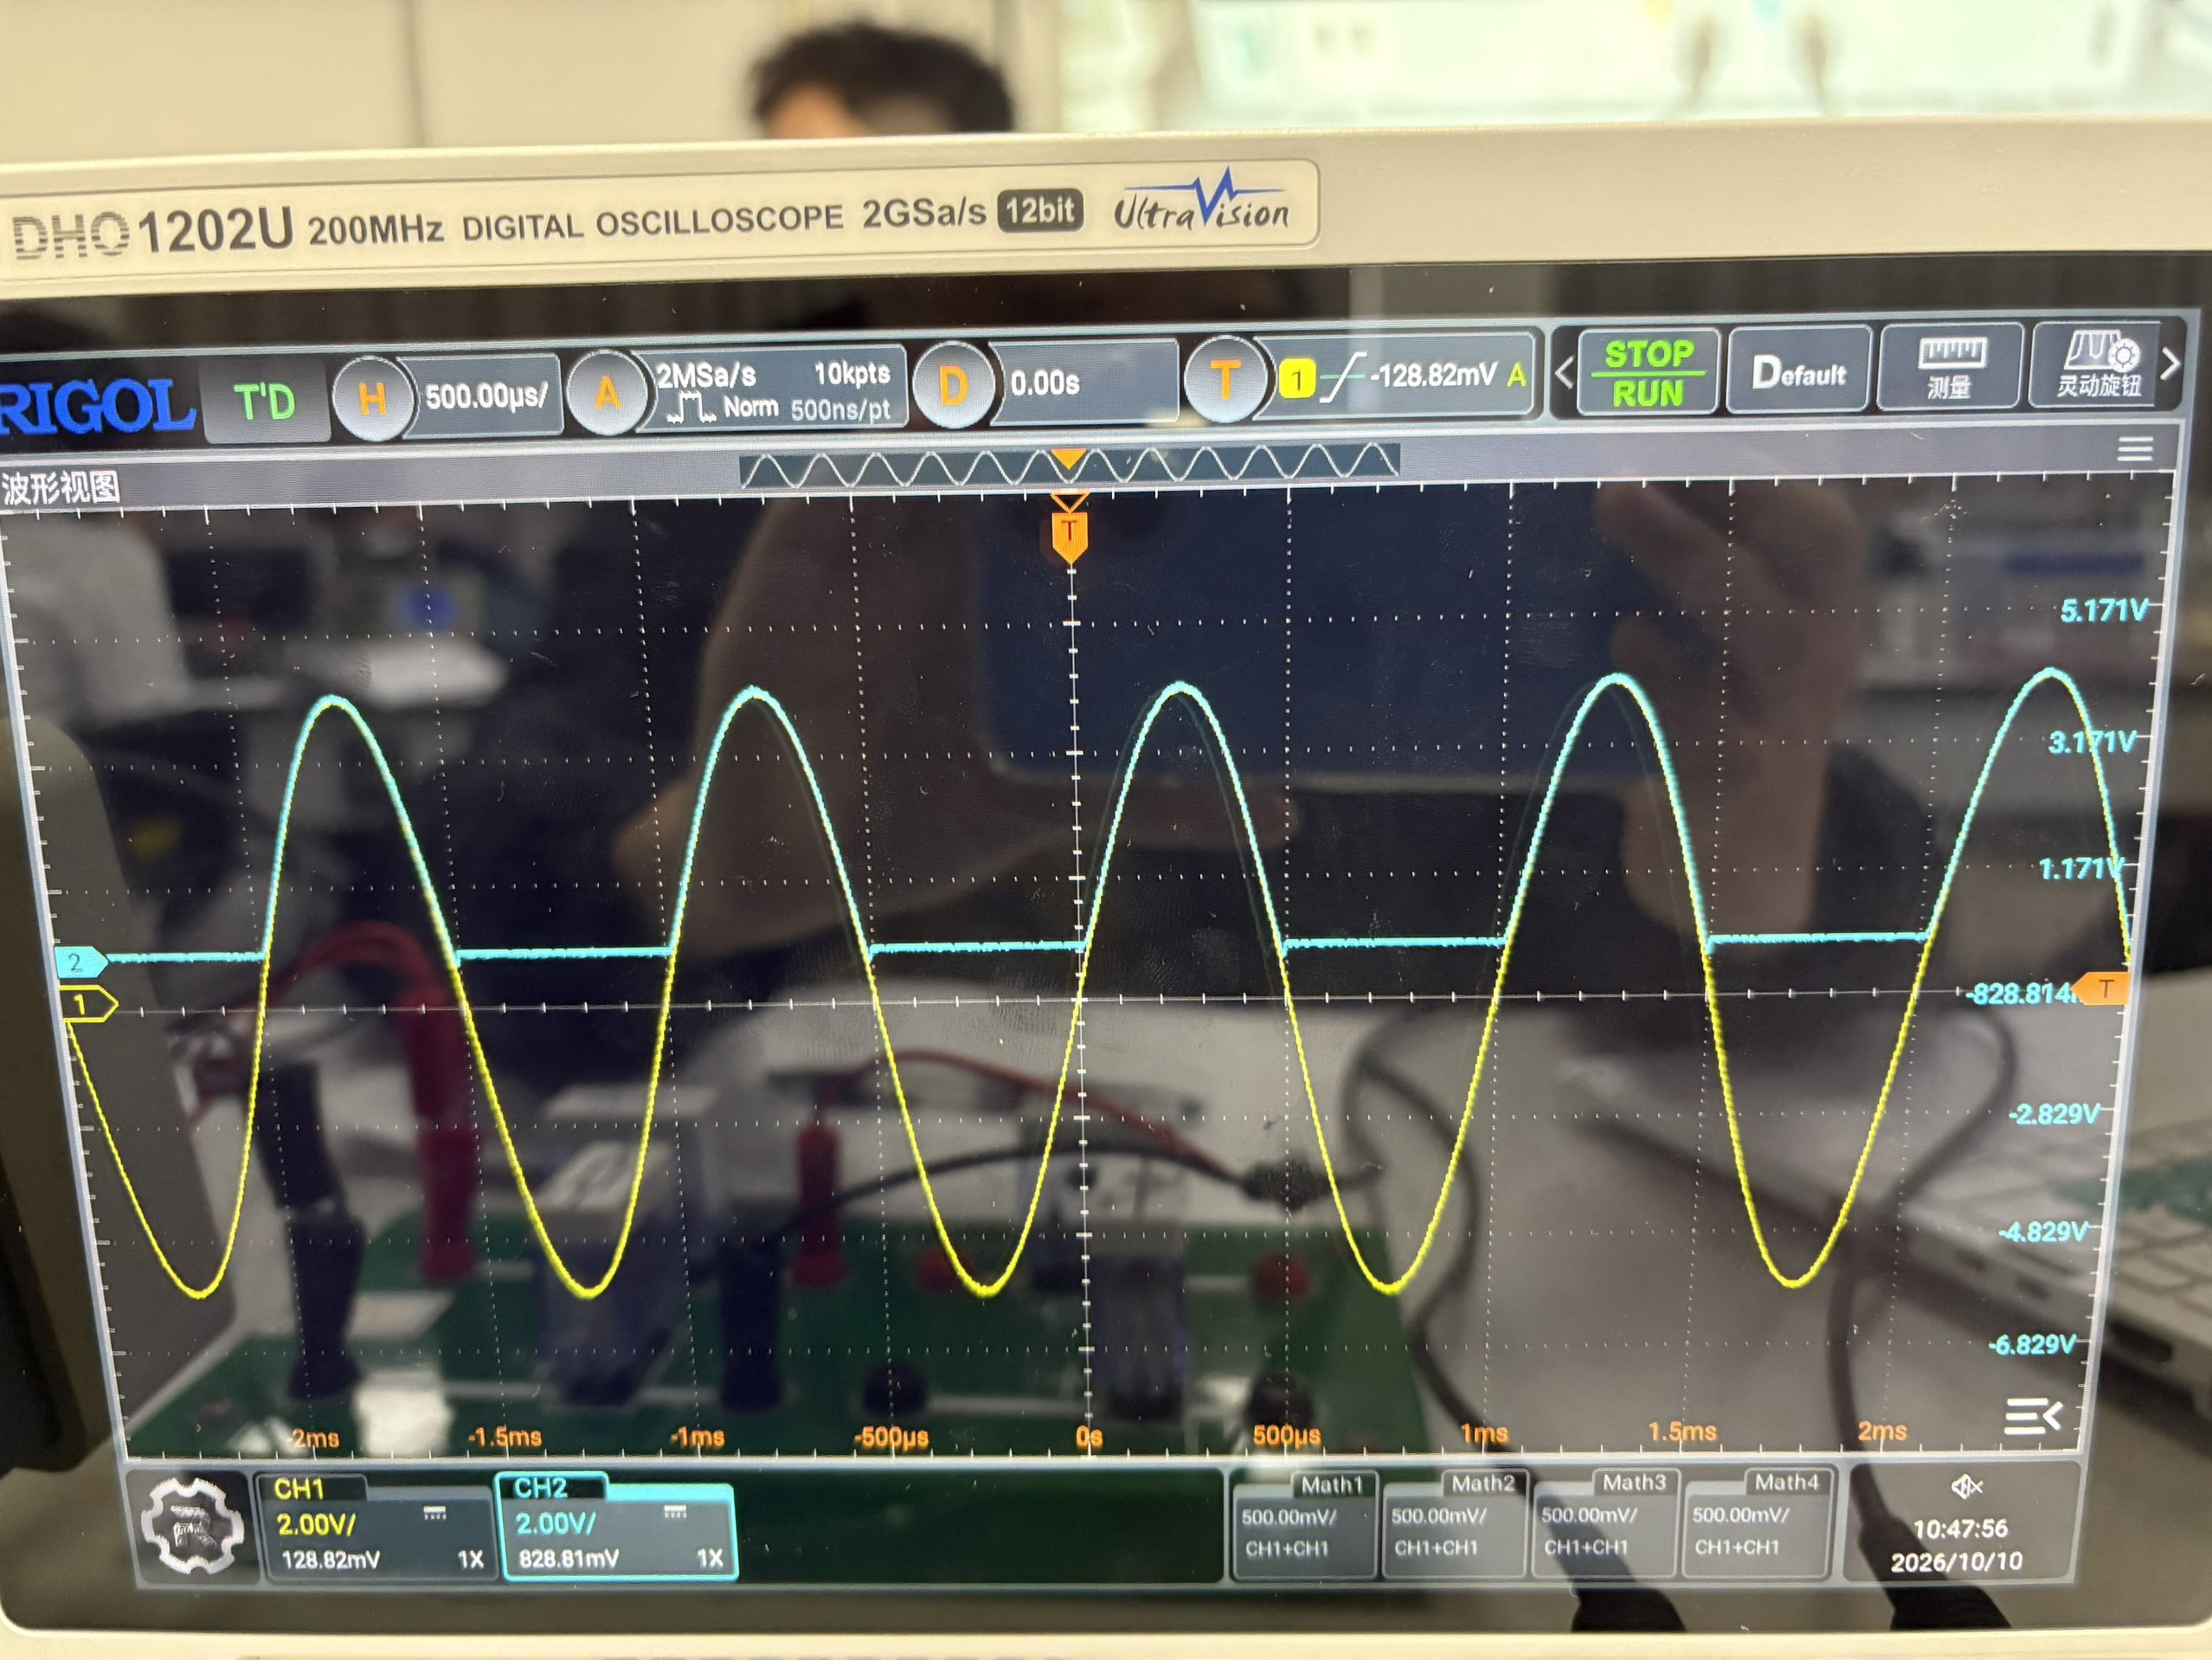
\includegraphics[width=0.8\textwidth]{figures/图10.png}
        \caption{二极管正向导通电压测量2}
      \end{minipage}
    \end{figure}

    分别运用Measure自动测量和光标测量得到以下结果，
    分别根据公式$U_{\text{导通}} = \frac{1}{2} U_{1p-p} - U_{2p}$和$U_{\text{导通}} = \Delta Y$计算得到$U_{\text{导通}}$。

    \begin{table}[H]
      \centering
      \begin{minipage}[t]{0.65\textwidth}
        \centering
        \captionof{table}{Measure自动测量}
        \begin{tabular}{ccccccc}
          \toprule
          实验次数 & 1 & 2 & 3 & 4 & 5 & 6 \\
          \midrule
          $U_{\mathrm{1p-p}}\,(\mathrm{V})$ & 10.001 & 10.001 & 10.010 & 10.019 & 10.001 & 9.9965 \\
          $U_{\mathrm{2p}}\,(\mathrm{V})$ & 4.7301 & 4.3653 & 4.3698 & 4.3701 & 4.3701 & 4.3562 \\
          $U_{\text{导通}}\,(\mathrm{mV})$ & 630.4 & 635.2 & 635.2 & 639.4 & 630.4 & 642.3 \\
          \bottomrule
        \end{tabular}
      \end{minipage}
      \hfill
      \begin{minipage}[t]{0.27\textwidth}
        \centering
        \captionof{table}{光标测量}
        \begin{tabular}{cc}
          \toprule
          & 光标测量 \\
          \midrule
          $AY(\mathrm{mV})$ & 496.1 \\
          $BY(\mathrm{mV})$ & -125.0 \\
          $U_{\text{导通}}\,(\mathrm{mV})$ & 621.1 \\
          \bottomrule
        \end{tabular}
      \end{minipage}
    \end{table}

    可见Measure和光标测量之间存在一定误差，但误差并不大。

    实验二：测量RC电路的相位差

    \begin{figure}[H]
      \centering
      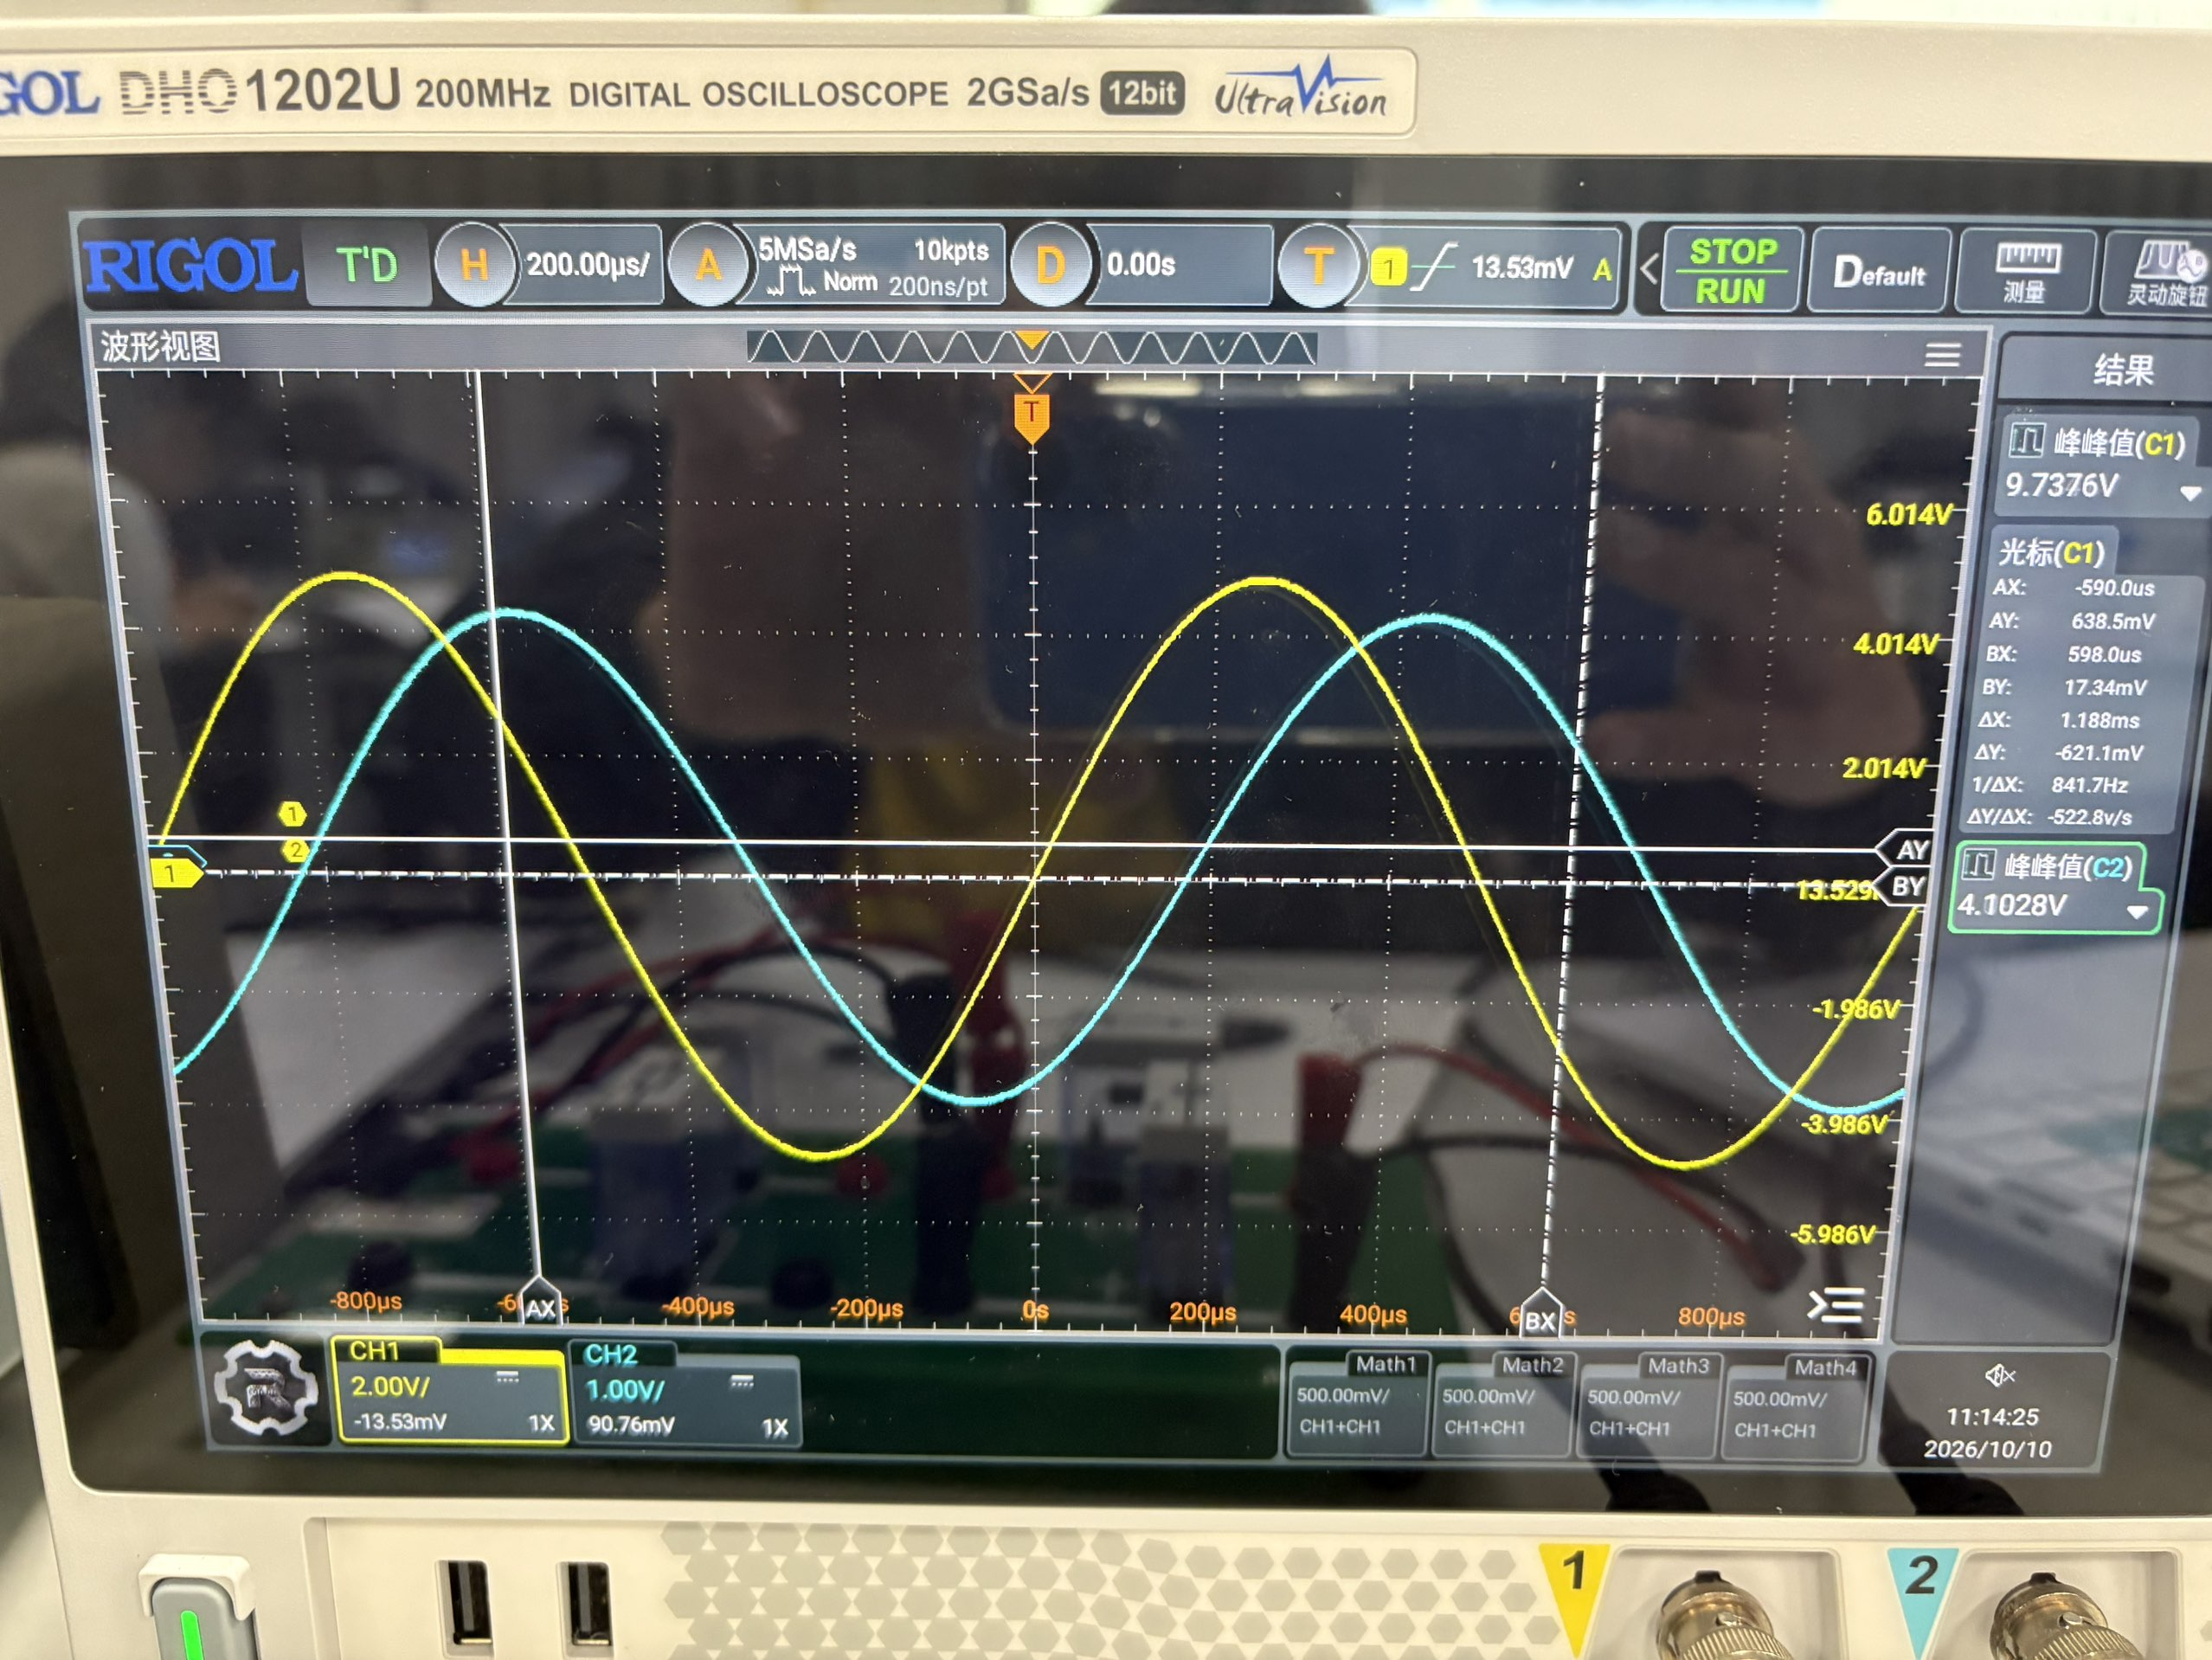
\includegraphics[width=0.4\textwidth]{figures/图11.png}
      \caption{测量RC电路的相位差}
    \end{figure}

    分别运用Measure自动测量和光标测量得到以下结果，

    \begin{table}[H]
      \centering
      \begin{minipage}[t]{0.58\textwidth}
        \centering
        \captionof{table}{Measure自动测量}
        \begin{tabular}{cc}
          \toprule
          & Measure自动测量 \\
          \midrule
          $\varphi_{\mathrm{r-r}}\,({}^\circ)$ & 64.812 \\
          $\varphi_{\mathrm{f-f}}\,({}^\circ)$ & 65.317 \\
          \bottomrule
        \end{tabular}
      \end{minipage}
      \hfill
      \begin{minipage}[t]{0.38\textwidth}
        \centering
        \captionof{table}{光标测量}
        \begin{tabular}{cc}
          \toprule
          & 光标测量 \\
          \midrule
          $T(\mathrm{ms})$ & 1.002 \\
          $\Delta t\,(\mu\mathrm{s})$ & 180.0 \\
          \bottomrule
        \end{tabular}
      \end{minipage}
    \end{table}

    光标法根据公式$\Delta \phi = \frac{\Delta t}{T} \times 360^\circ$计算得到$\Delta \phi$，
    即
    $\Delta \varphi
    = \frac{\Delta t}{T} \times 360^\circ
    = \frac{180.0 \times 10^{-6}}{1.002 \times 10^{-3}} \times 360^\circ
    = 64.67^\circ$。
    而Measure自动测量直接给出的相位差平均值为$\frac{64.812^\circ + 65.317^\circ}{2} = 65.0645^\circ$。 
    可见光标法和Measure自动测量的结果接近。

    实验三：李萨如图形测量未知信号的频率

    Measure直接测量的结果为50.226Hz，利用李萨如图形测量的实验结果如下，其中$f_y$由公式$f_y = \frac{n_x}{n_y} f_x$得到。

    \begin{table}[H]
      \centering
      \caption{李萨如图形测量未知信号的频率}
      \begin{tabular}{ccccccc}
        \toprule
        $f_y:f_x$ & $1:1$ & $1:2$ & $1:3$ & $2:1$ & $3:1$ & $2:3$ \\
        \midrule
        图形 & 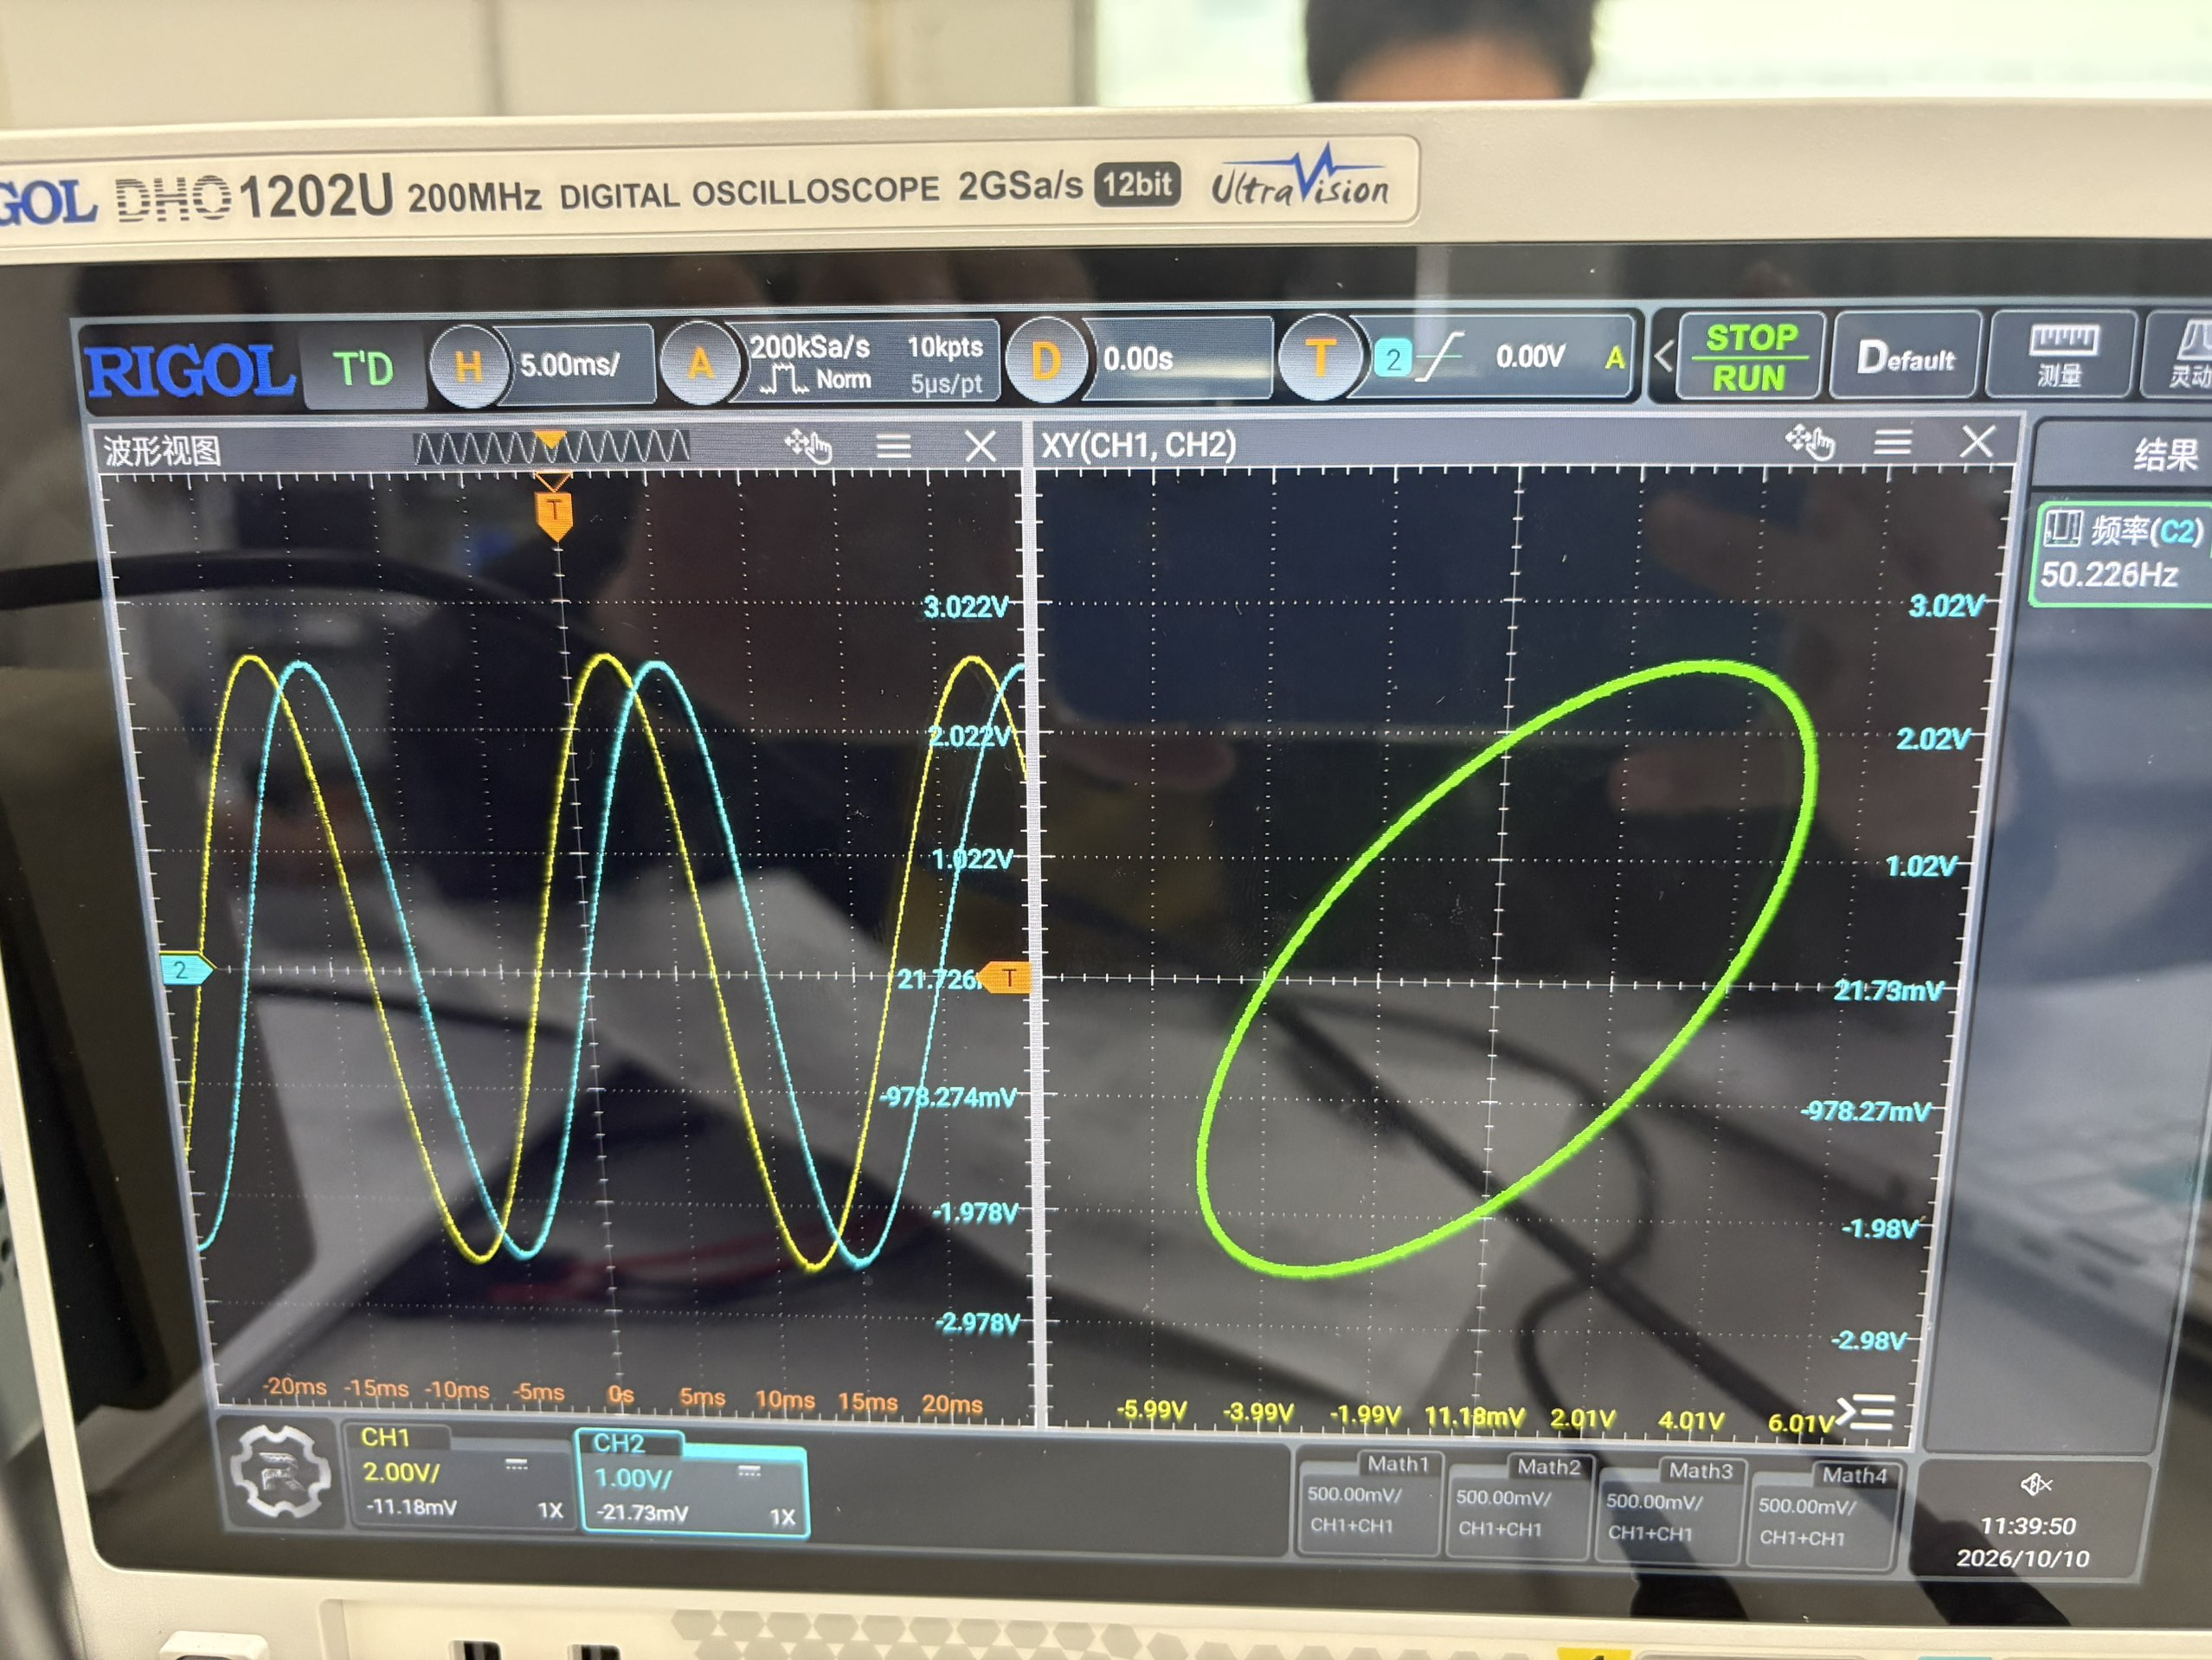
\includegraphics[width=0.1\textwidth]{figures/图12.png} & 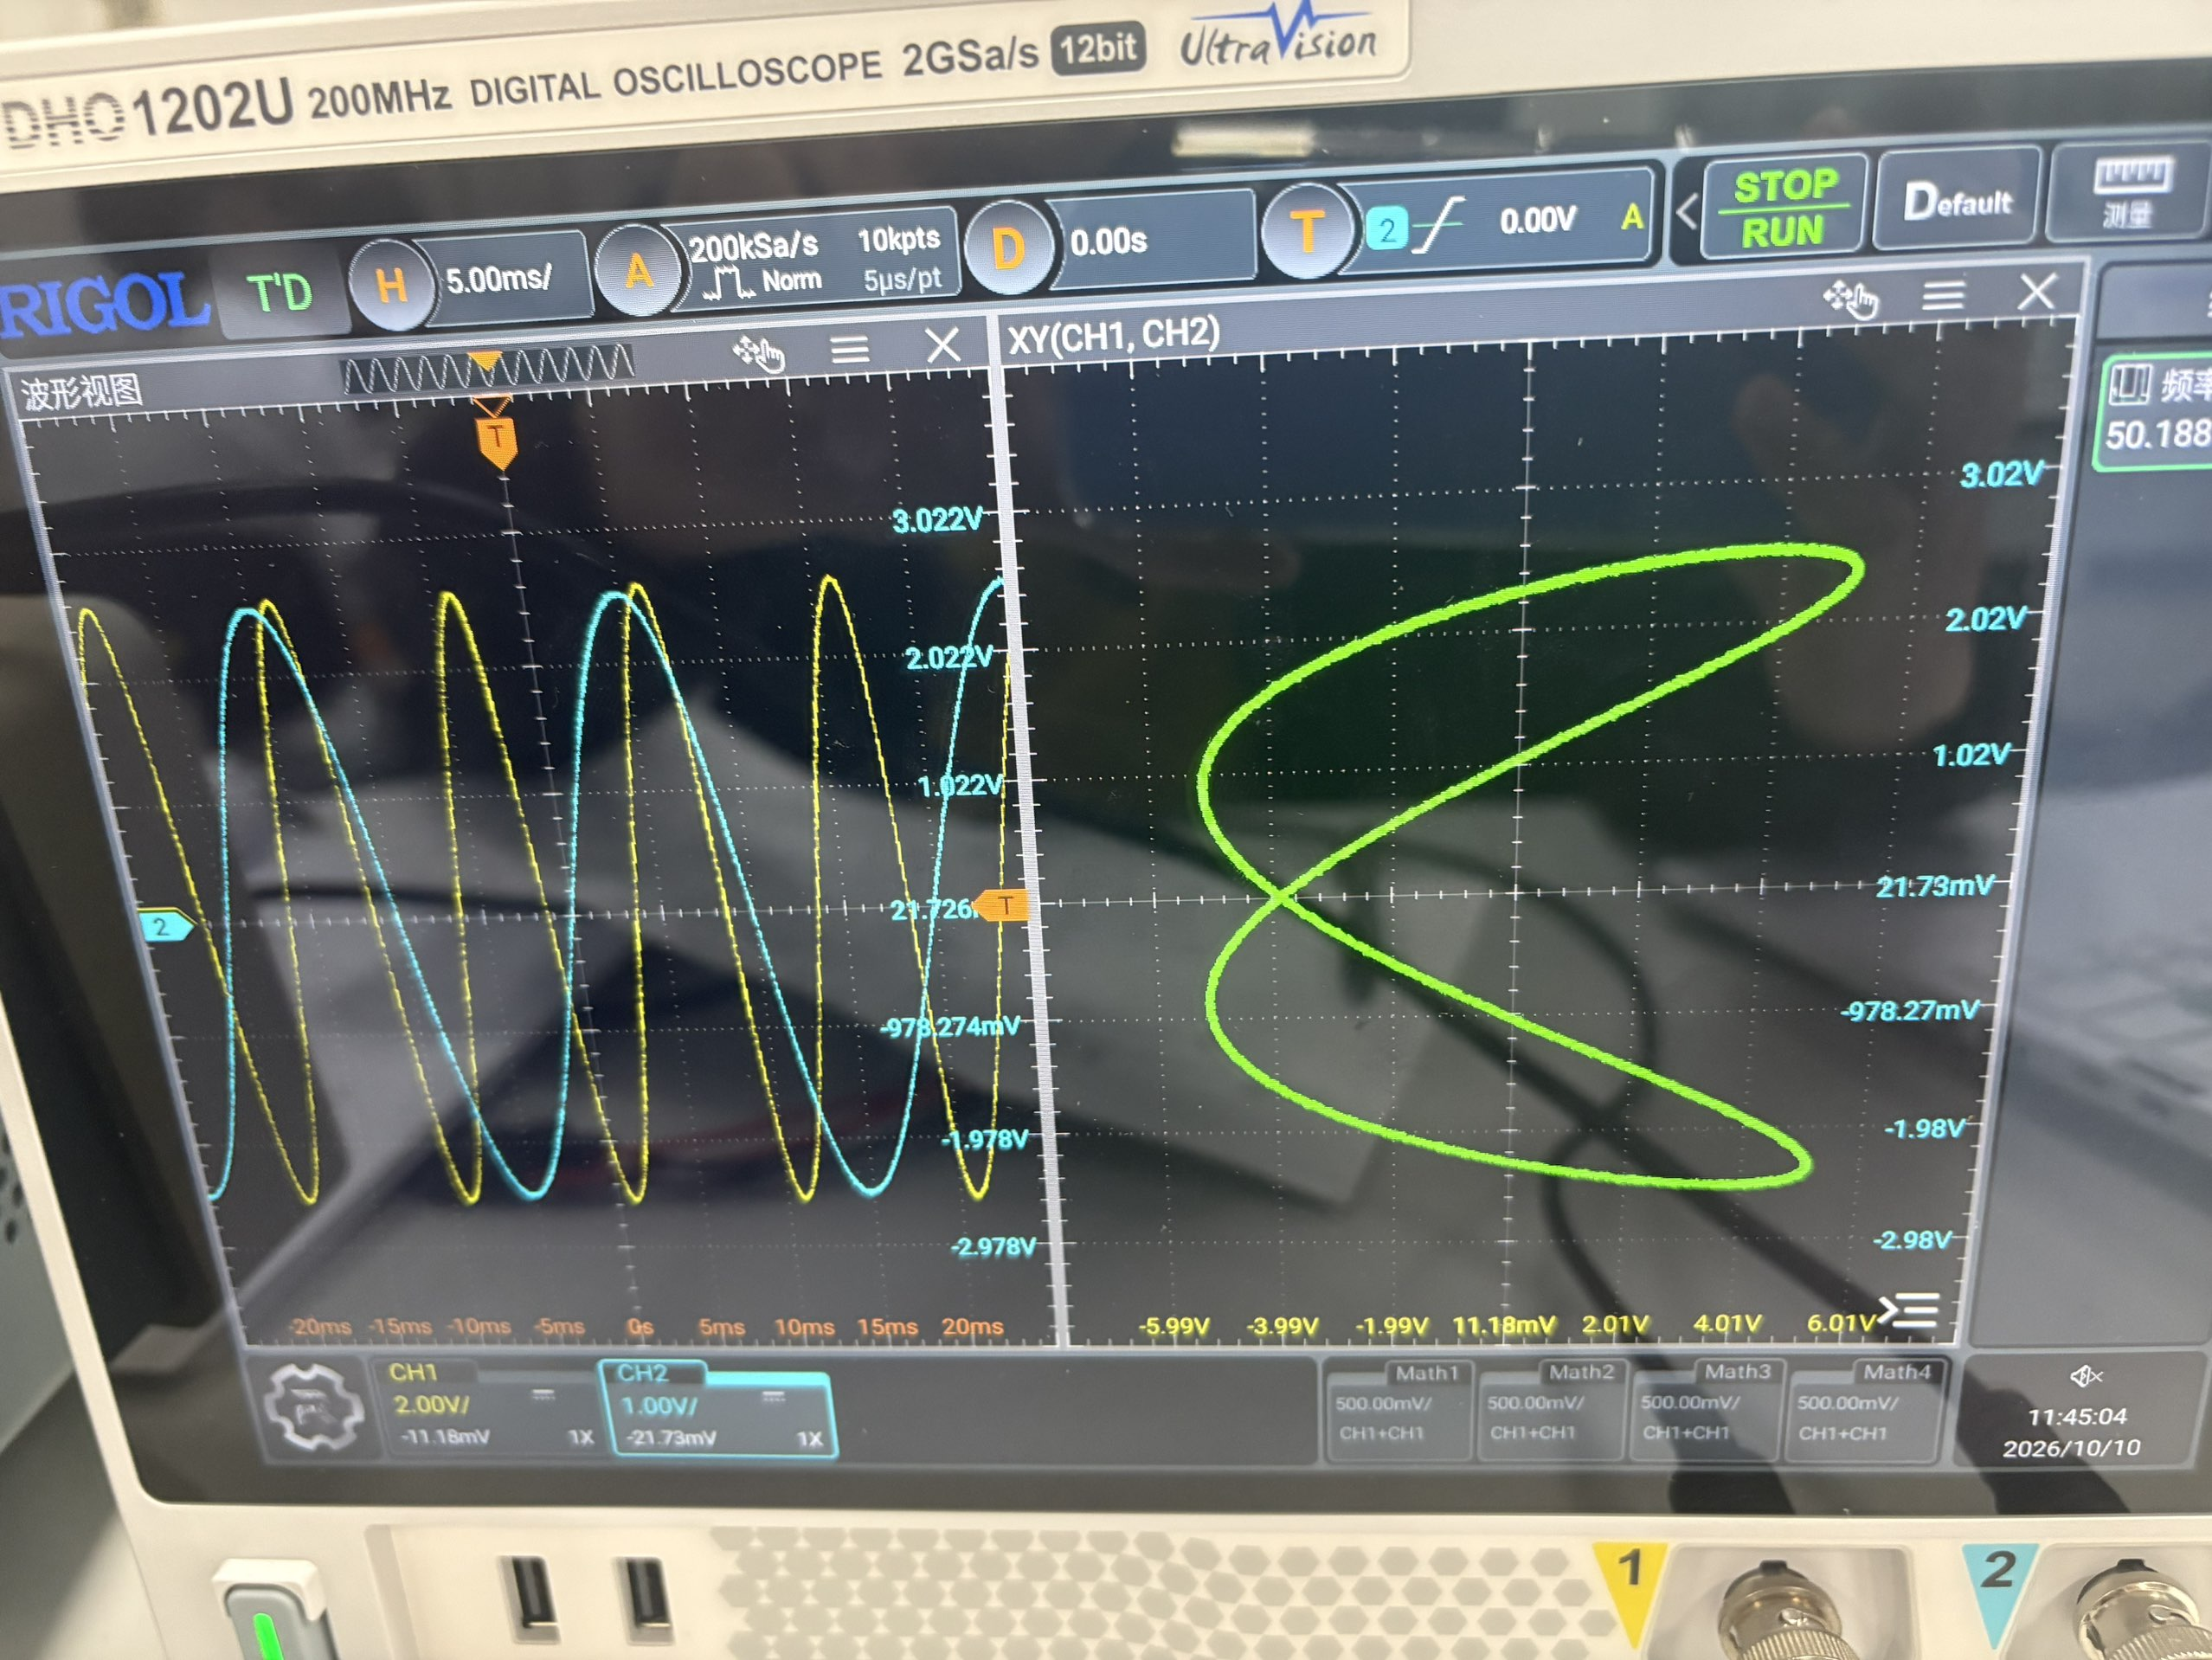
\includegraphics[width=0.1\textwidth]{figures/图13.png} 
            & 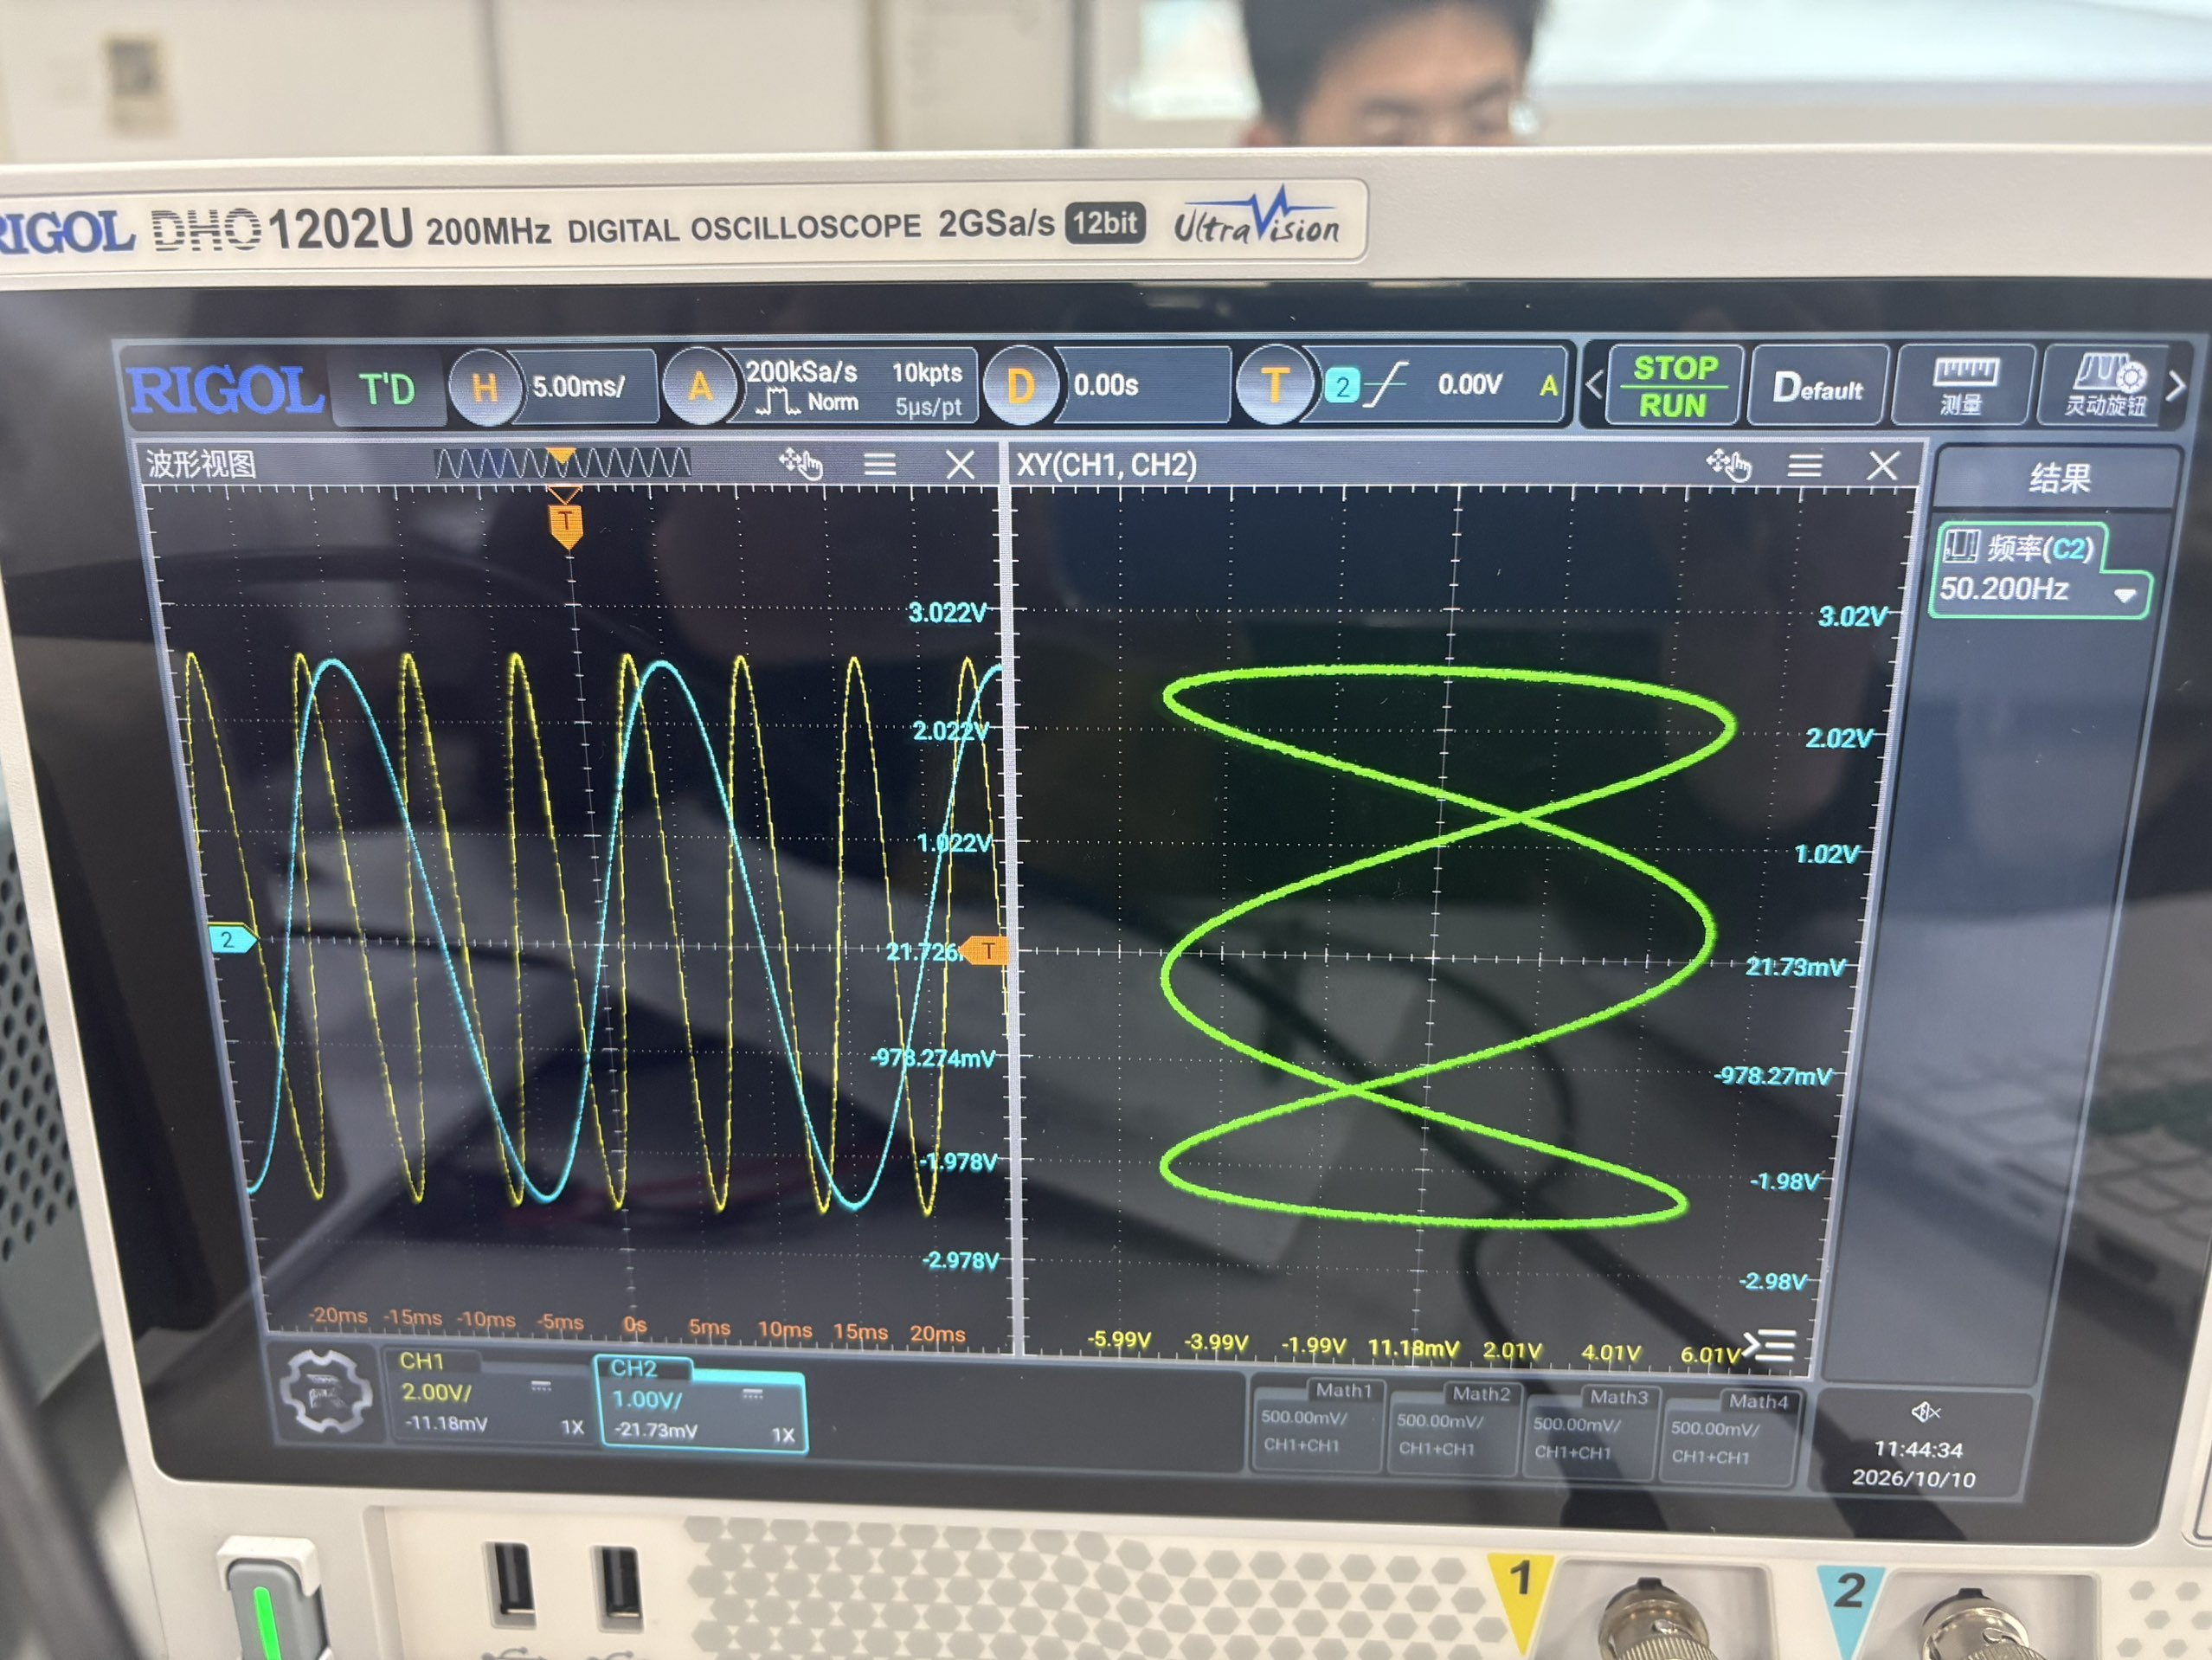
\includegraphics[width=0.1\textwidth]{figures/图14.png} & 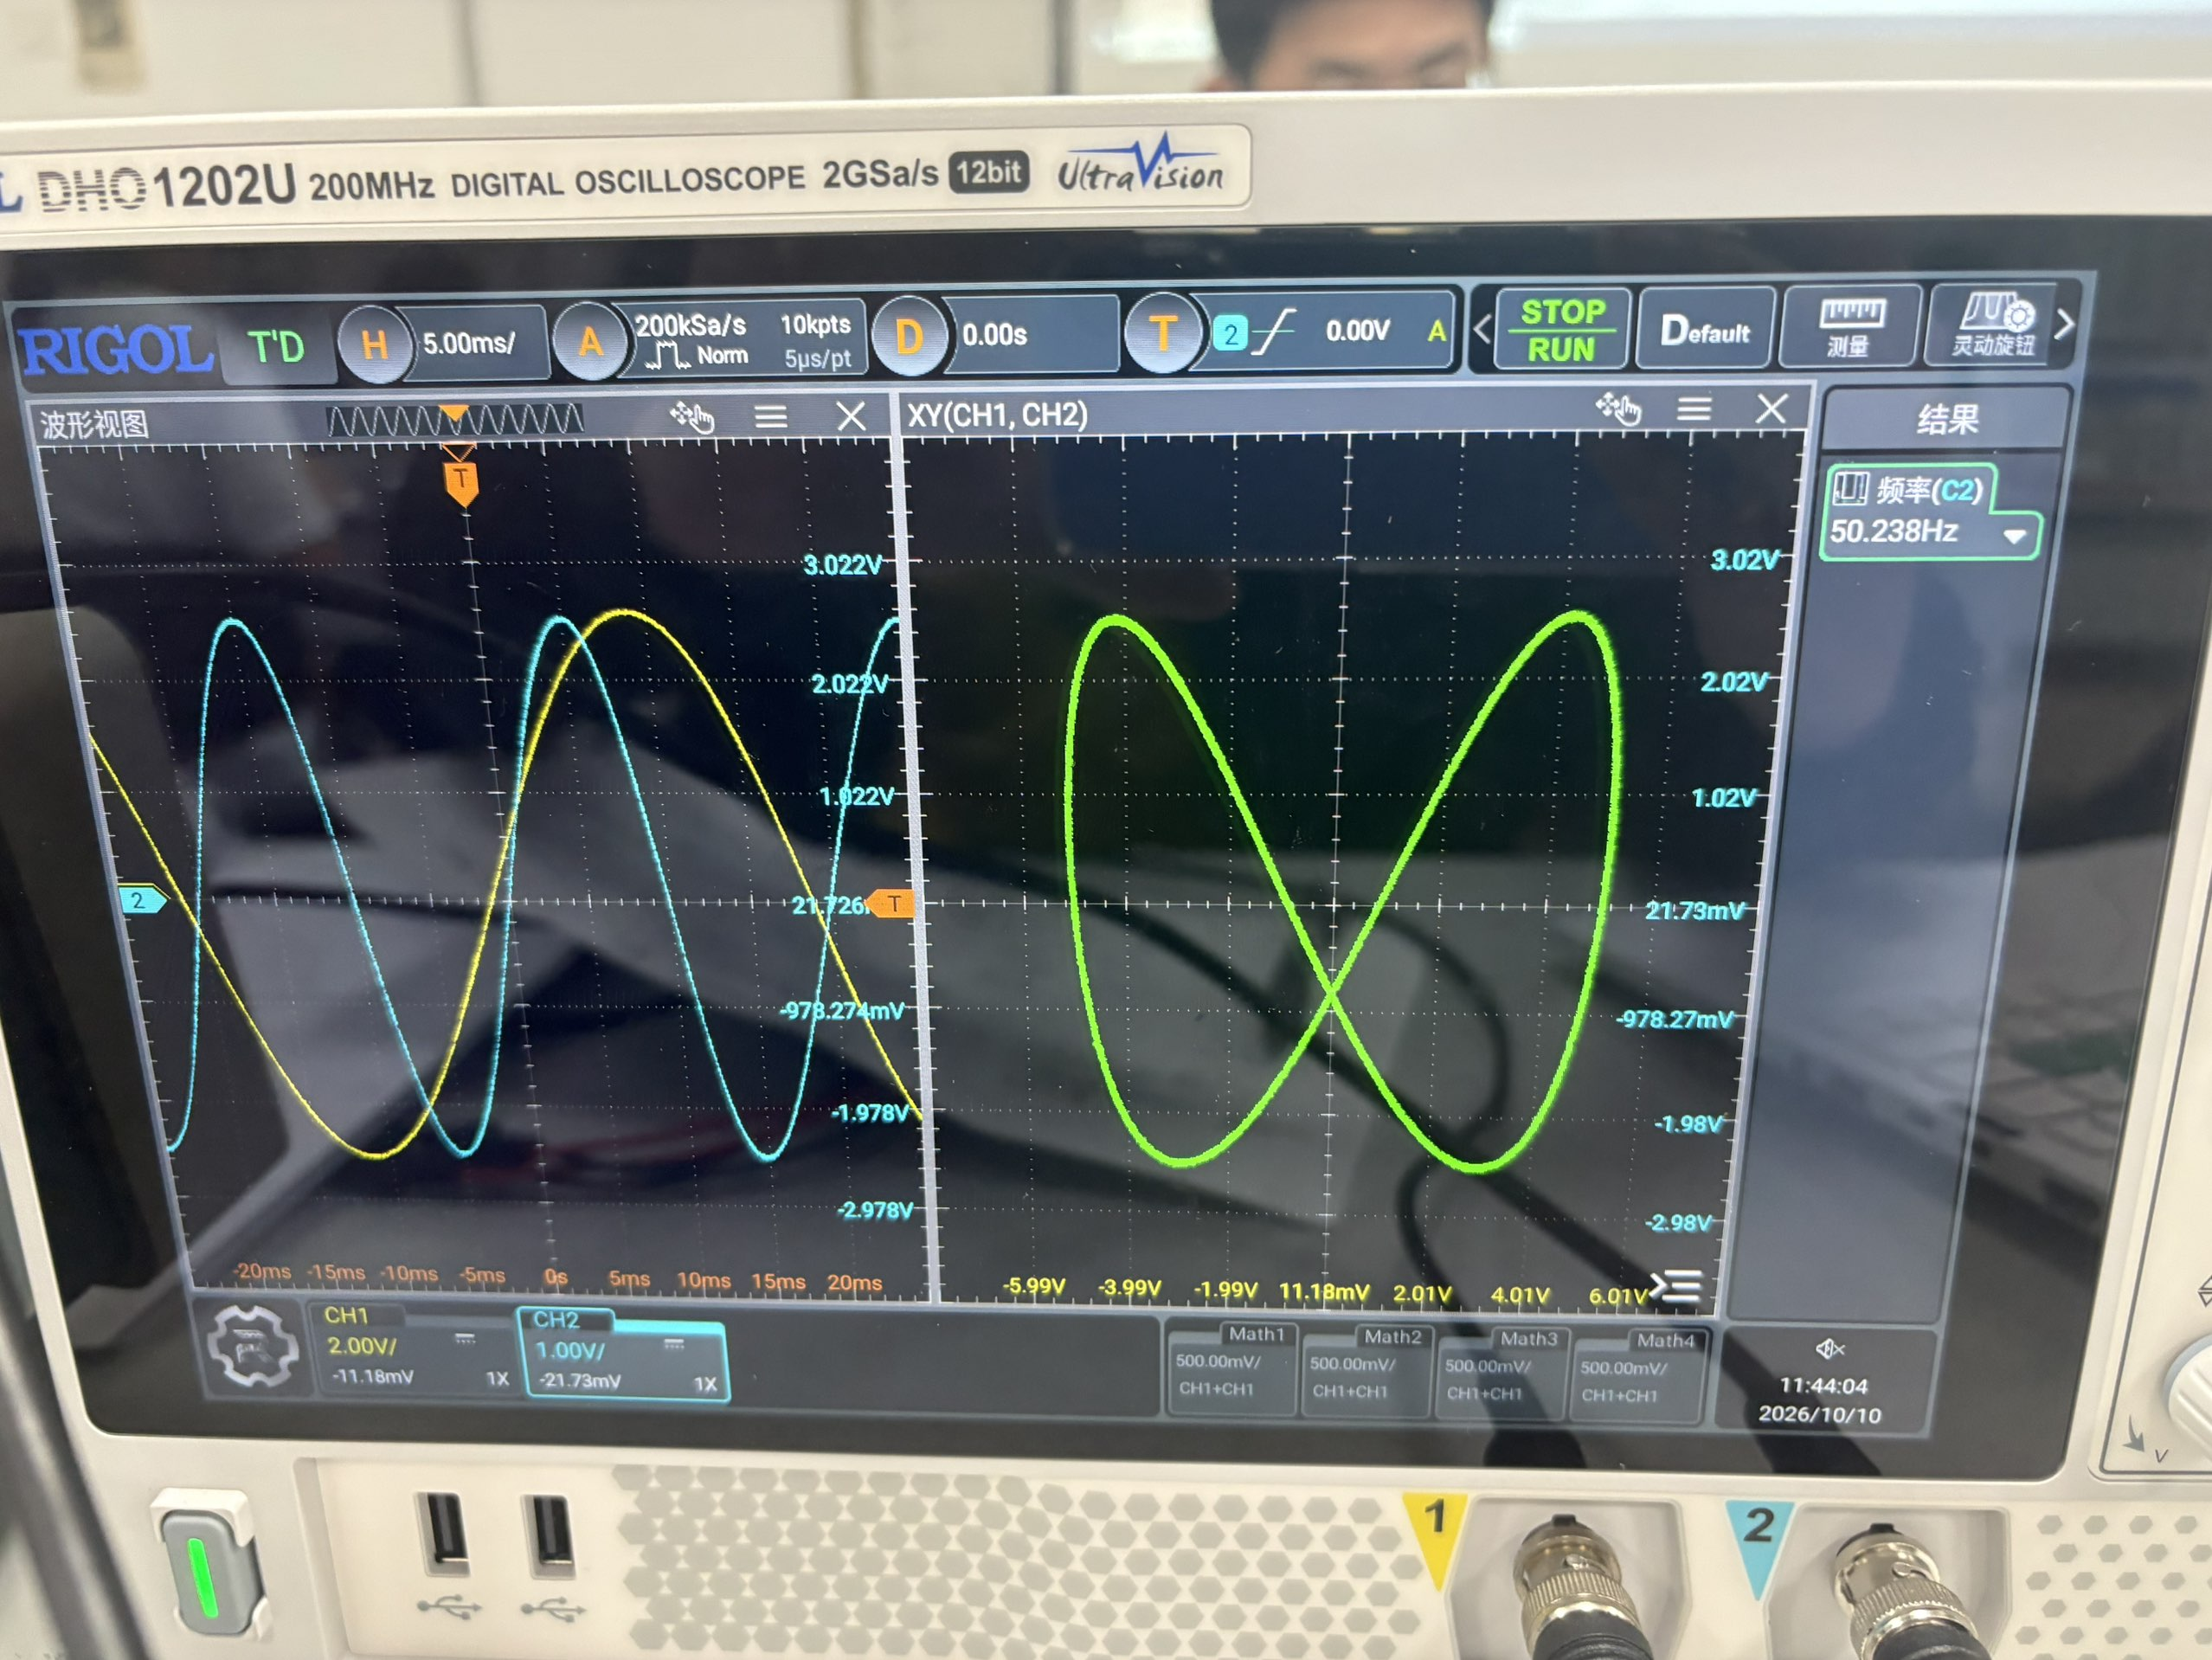
\includegraphics[width=0.1\textwidth]{figures/图15.png} 
            & 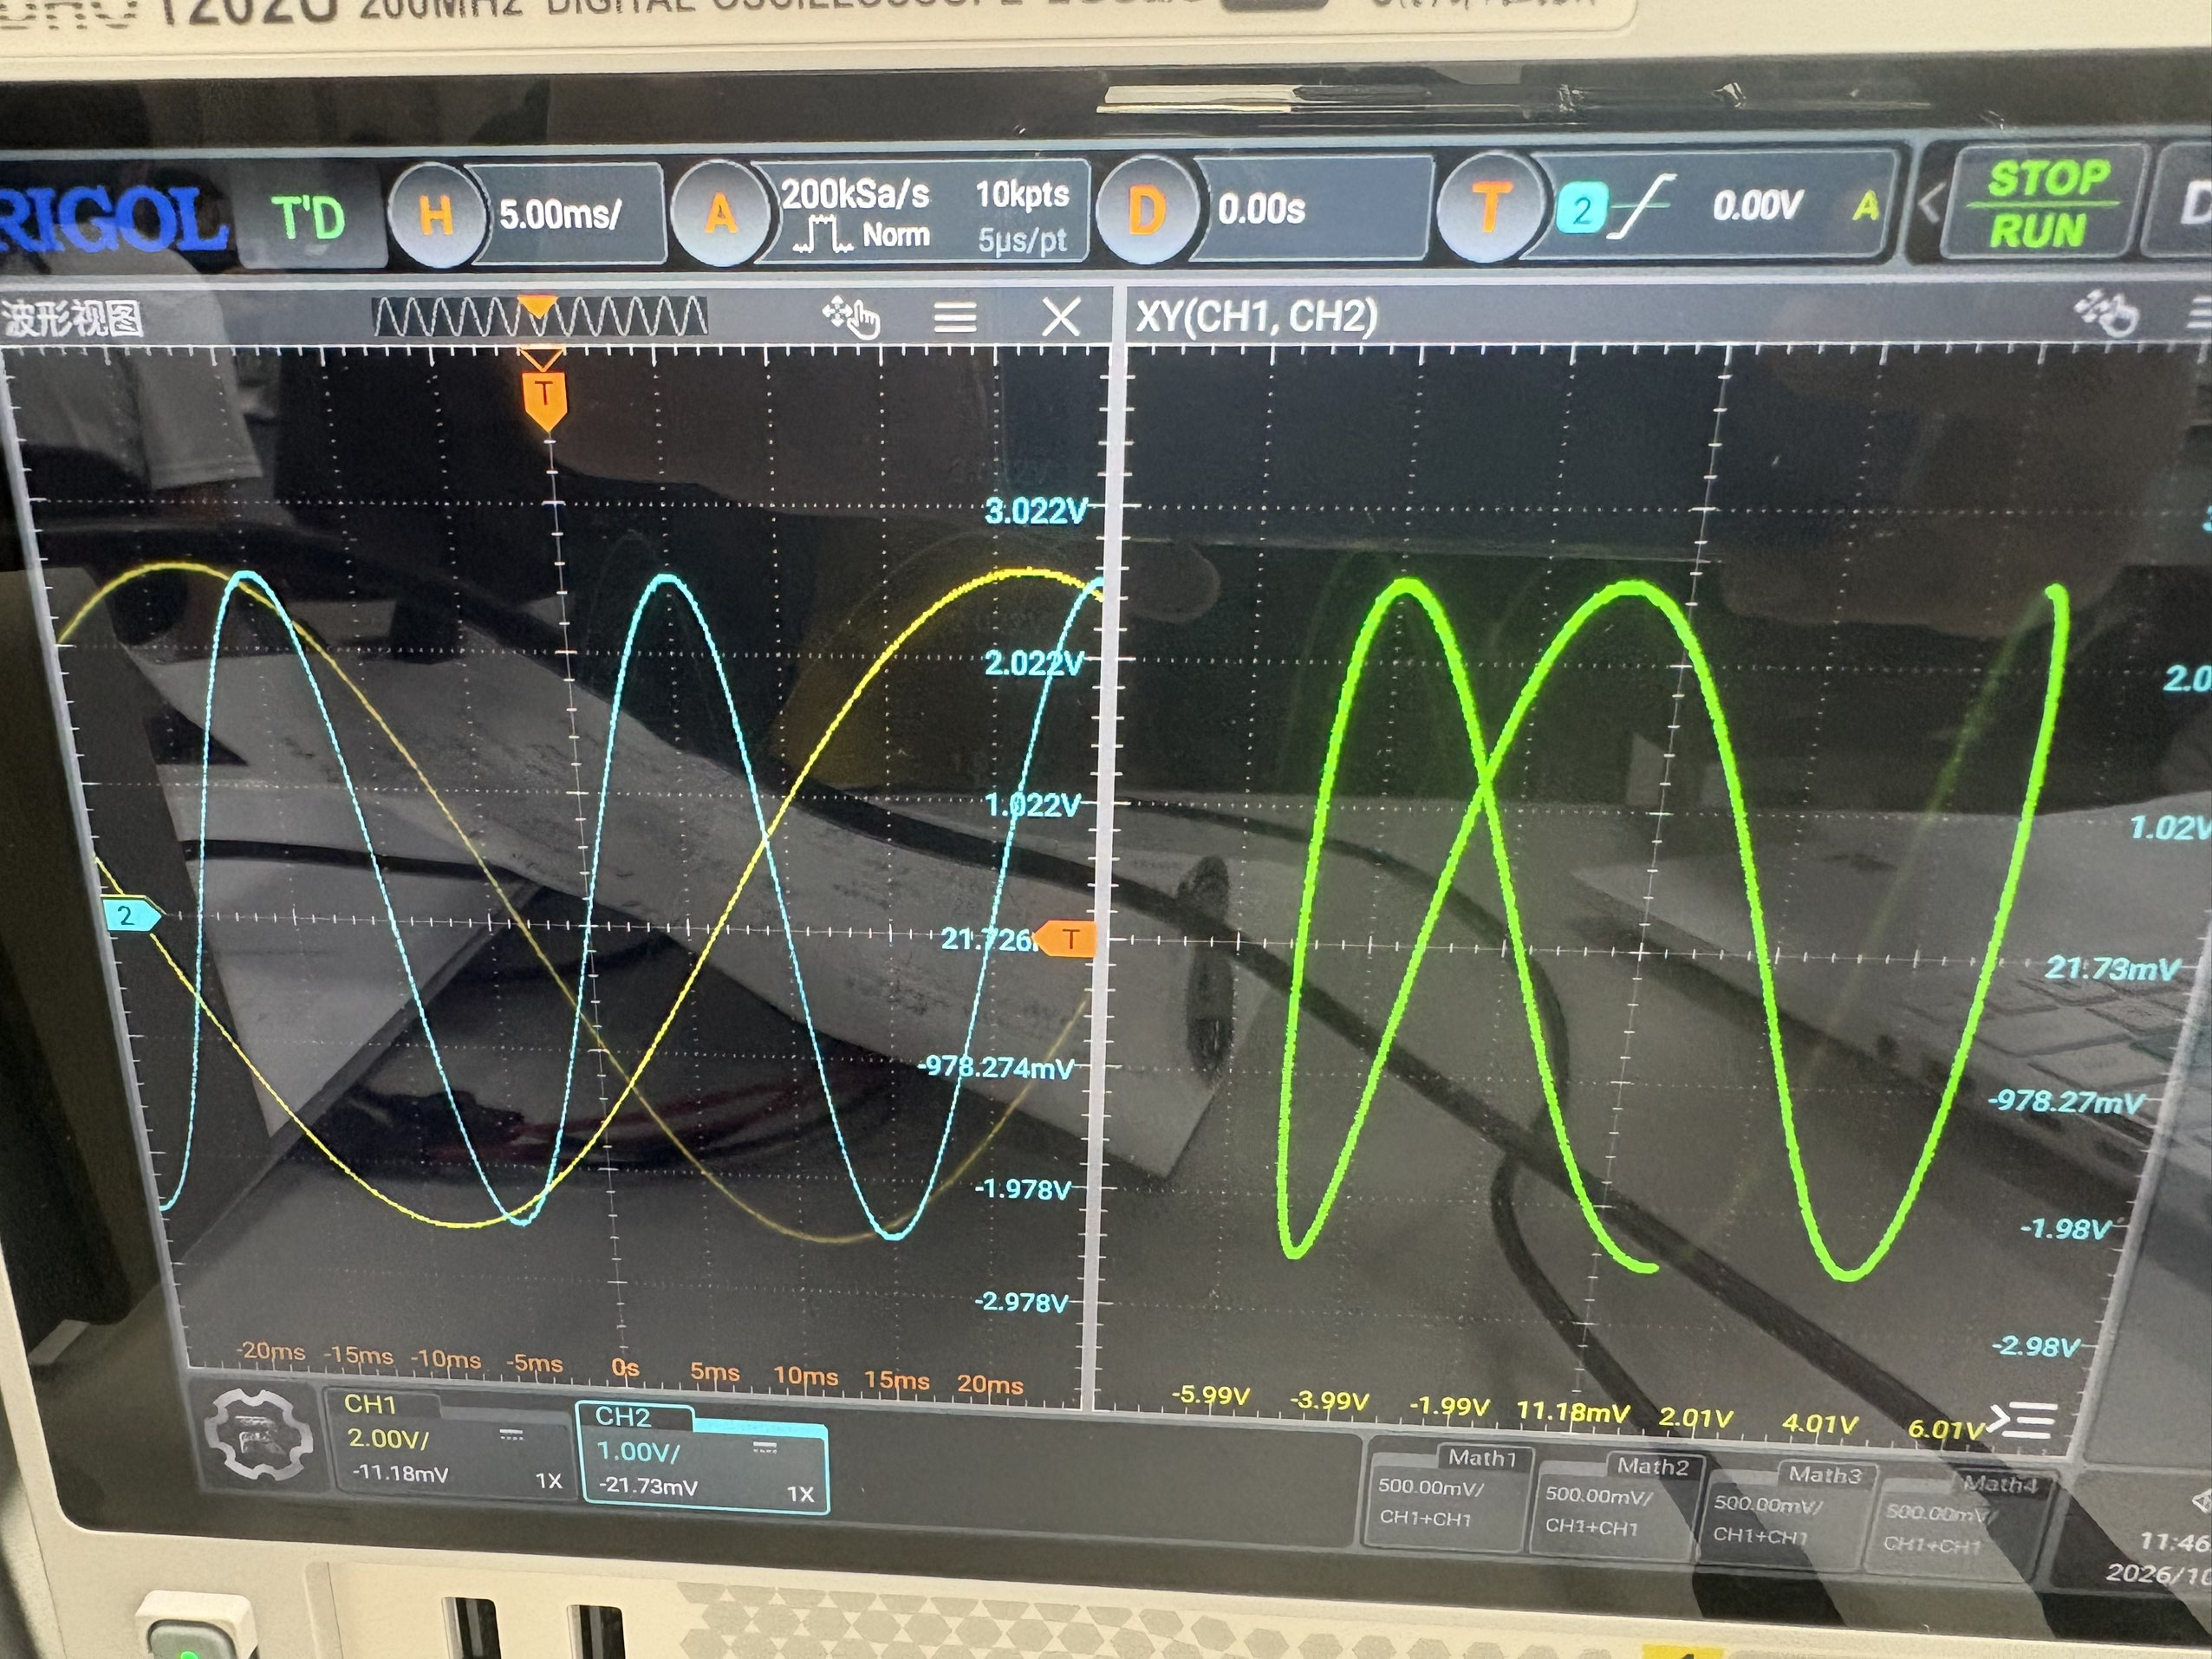
\includegraphics[width=0.1\textwidth]{figures/图16.png} & 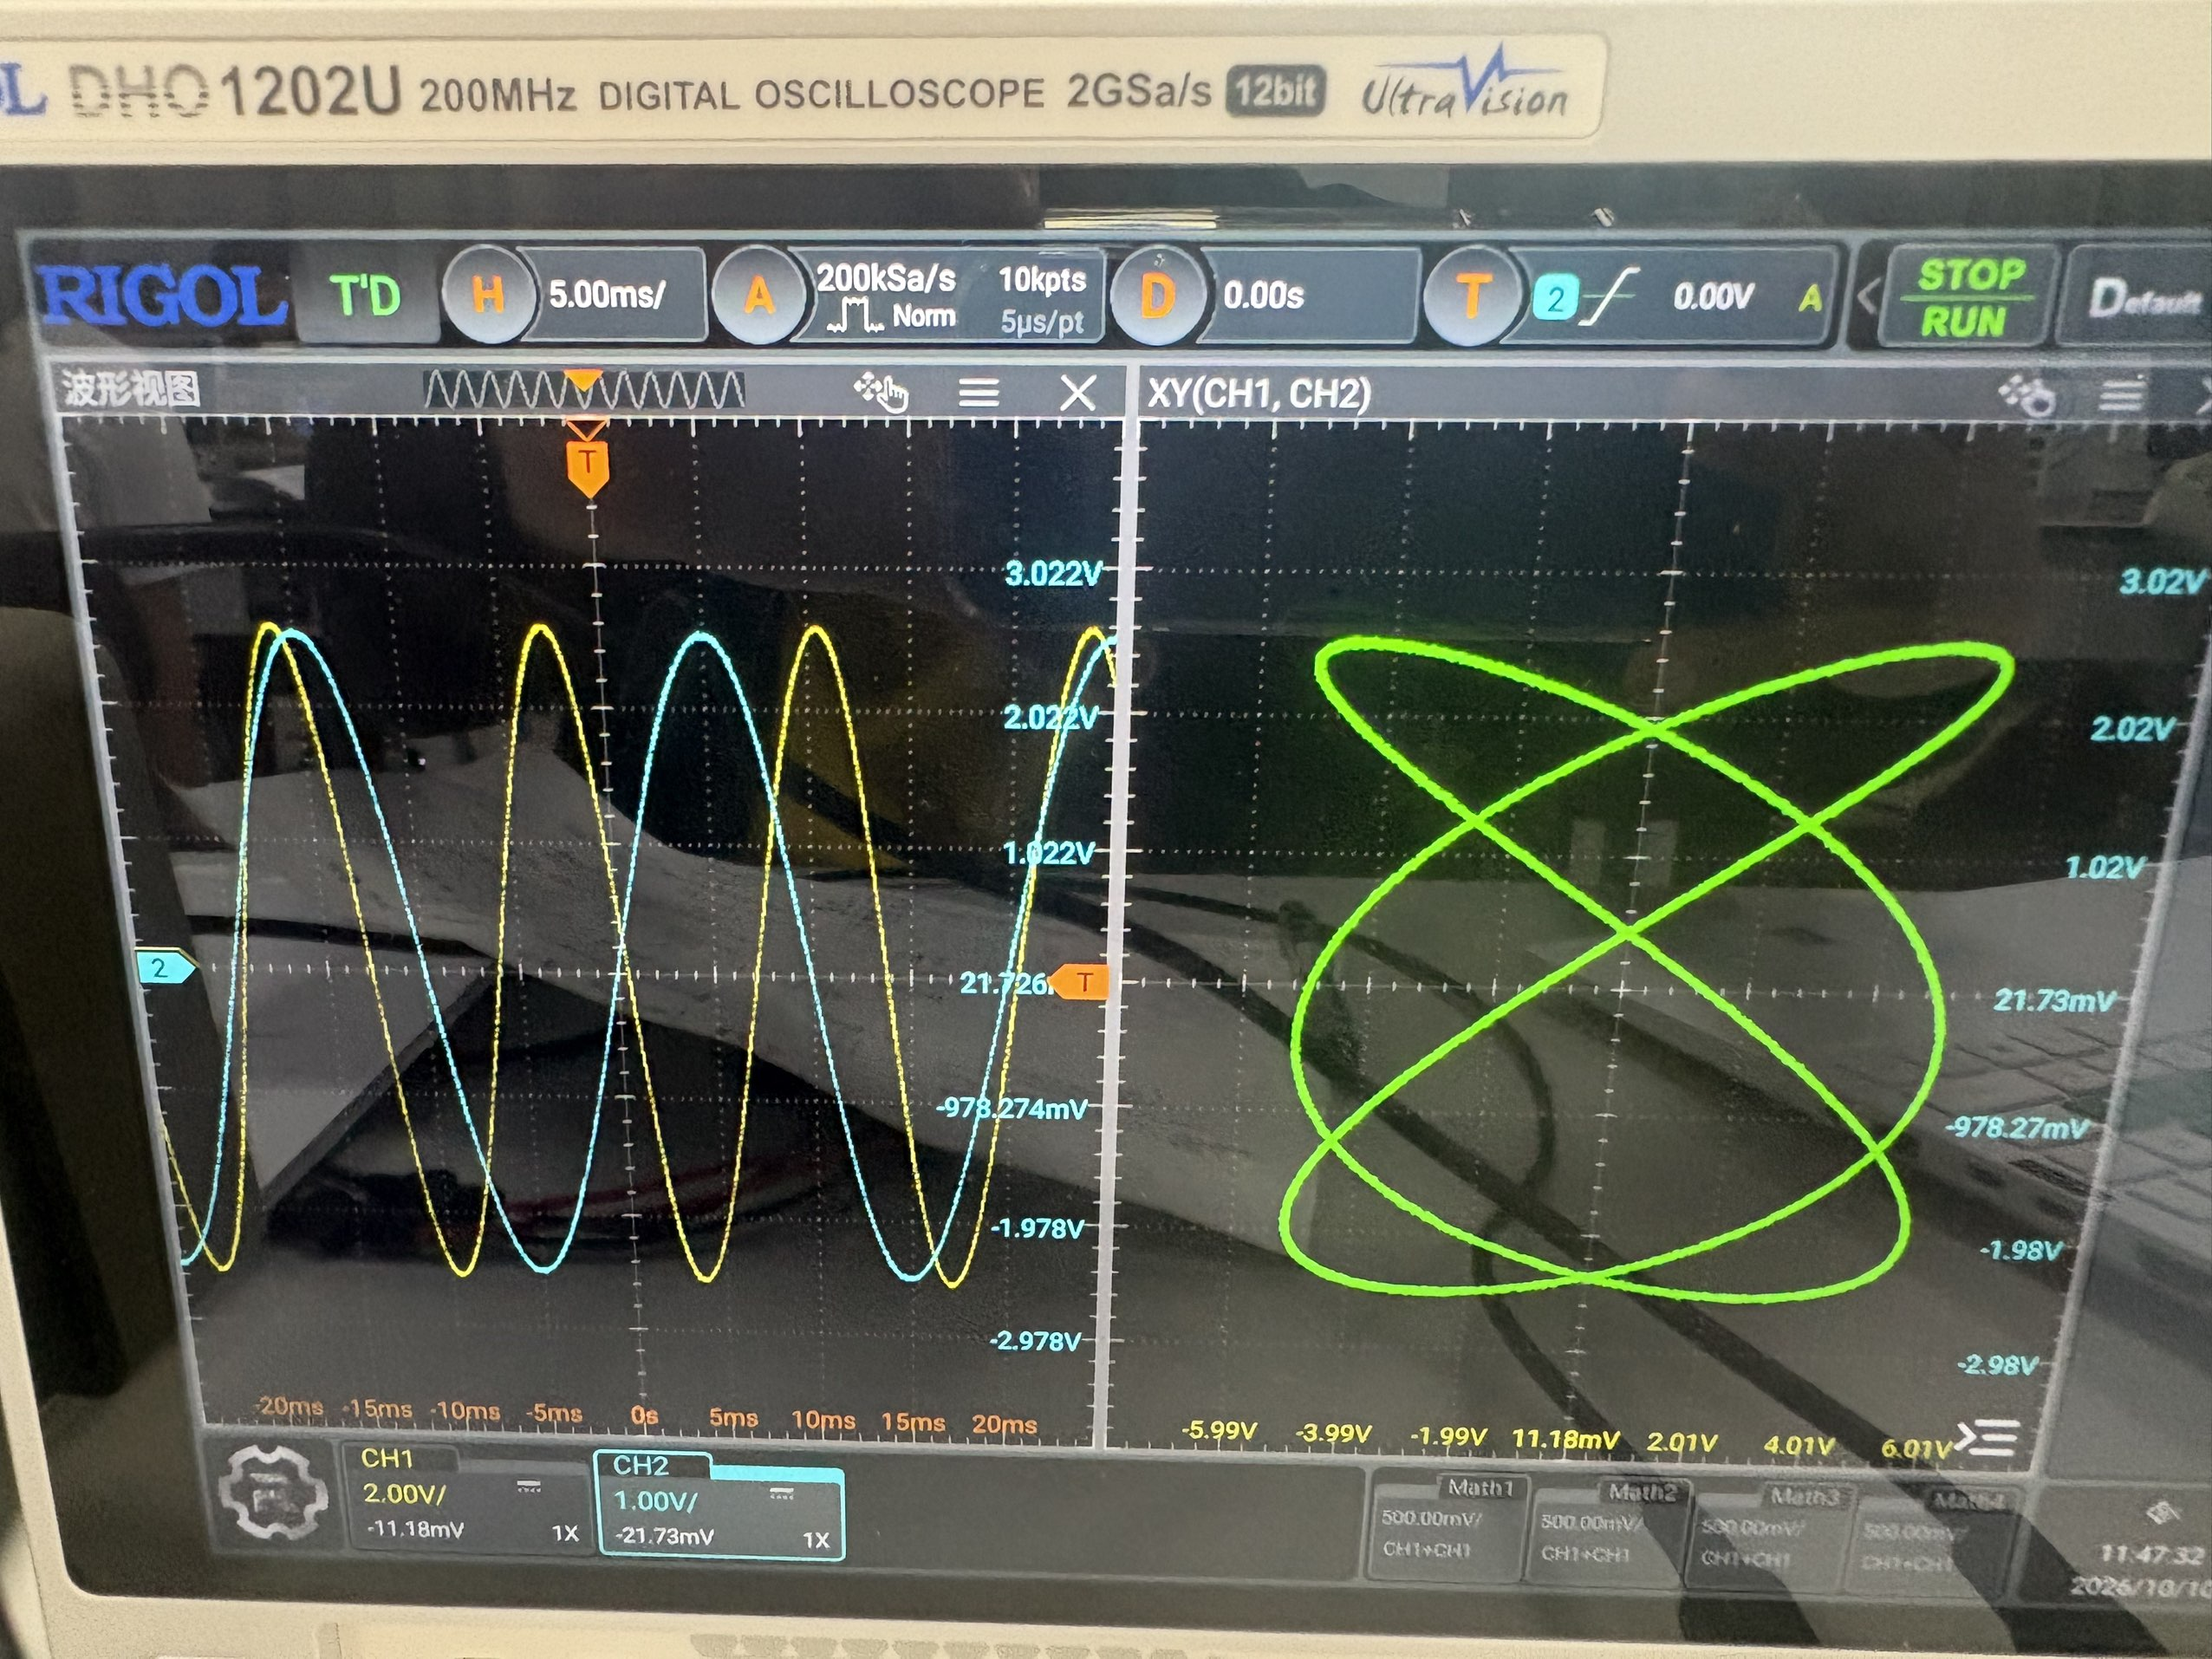
\includegraphics[width=0.1\textwidth]{figures/图17.png} \\
        垂直交点数$n_y$ & 2 & 4 & 6 & 2 & 2 & 6 \\
        水平交点数$n_x$ & 2 & 2 & 2 & 4 & 6 & 4 \\
        $f_x\,(\mathrm{Hz})$ & 50.2324 & 100.4721 & 150.7021 & 25.1200 & 16.7432 & 75.3522 \\
        $f_y\,(\mathrm{Hz})$ & 50.2324 & 50.2361 & 50.2340 & 50.2400 & 50.2296 & 50.2348 \\
        \bottomrule
      \end{tabular}
    \end{table}

    为综合六组李萨如图形的测频结果，取所测频率的平均值作为未知频率的估计值：
    \[
    \begin{aligned}
    \overline{f}_y
    &= \frac{1}{6}\sum_{i=1}^{6}f_{yi} \\
    &= \frac{50.2324+50.2361+50.2340+50.2400+50.2296+50.2348}{6}
      \,\mathrm{Hz} \\
    &= 50.2345\,\mathrm{Hz}
    \end{aligned}
    \]

    为进一步描述各组测量结果的离散程度，以平均频率计算样本标准差：
    \[
    \begin{aligned}
    s(f_y)
    &= \sqrt{
    \frac{\displaystyle\sum_{i=1}^{6}
    (f_{yi}-\overline{f}_y)^2}{6-1}
    } \\
    &= \sqrt{
    \frac{6.1568333\times10^{-5}}{5}
    }\,\mathrm{Hz} \\
    &= 0.00351\,\mathrm{Hz}
    \end{aligned}
    \]

    假设测量期间未知频率稳定，各组换算结果相互独立且精度近似相同，
    则平均频率的A类标准不确定度为：
    \[
    \begin{aligned}
    u_A(\overline{f}_y)
    &= \frac{s(f_y)}{\sqrt{6}}
     = \sqrt{\frac{\displaystyle\sum_{i=1}^{6}
       (f_{yi}-\overline{f}_y)^2}{6(6-1)}} \\
    &= \sqrt{\frac{6.1568333\times10^{-5}}{6\times5}}
       \,\mathrm{Hz} \\
    &= 0.00143\,\mathrm{Hz}
    \end{aligned}
    \]

    因此，平均频率为$\overline{f}_y=50.2345\,\mathrm{Hz}$，
    A类标准不确定度取$u_A(\overline{f}_y)=0.0014\,\mathrm{Hz}$。
    此处仅评估测量结果离散性对平均频率的影响，尚未计入仪器准确度等引入的B类不确定度。

    \subsubsection{组装整流器}
    实验分别搭建半波、全波、桥式三种整流电路，测得输入信号的有效值$U_2$和整流电路的信号平均值$\overline{U_0}$如下： 
    \begin{table}[H]
      \centering
      \caption{三种整流电路测量结果}
      \begin{tabular}{ccccc}
        \toprule
        整流电路类型 & $\overline{U_0}/\mathrm{V}$ & $U_2/\mathrm{V}$ & 输入波形 & 输出波形 \\
        \midrule
        单相半波整流电路 & 2.6125 & 5.9776 & 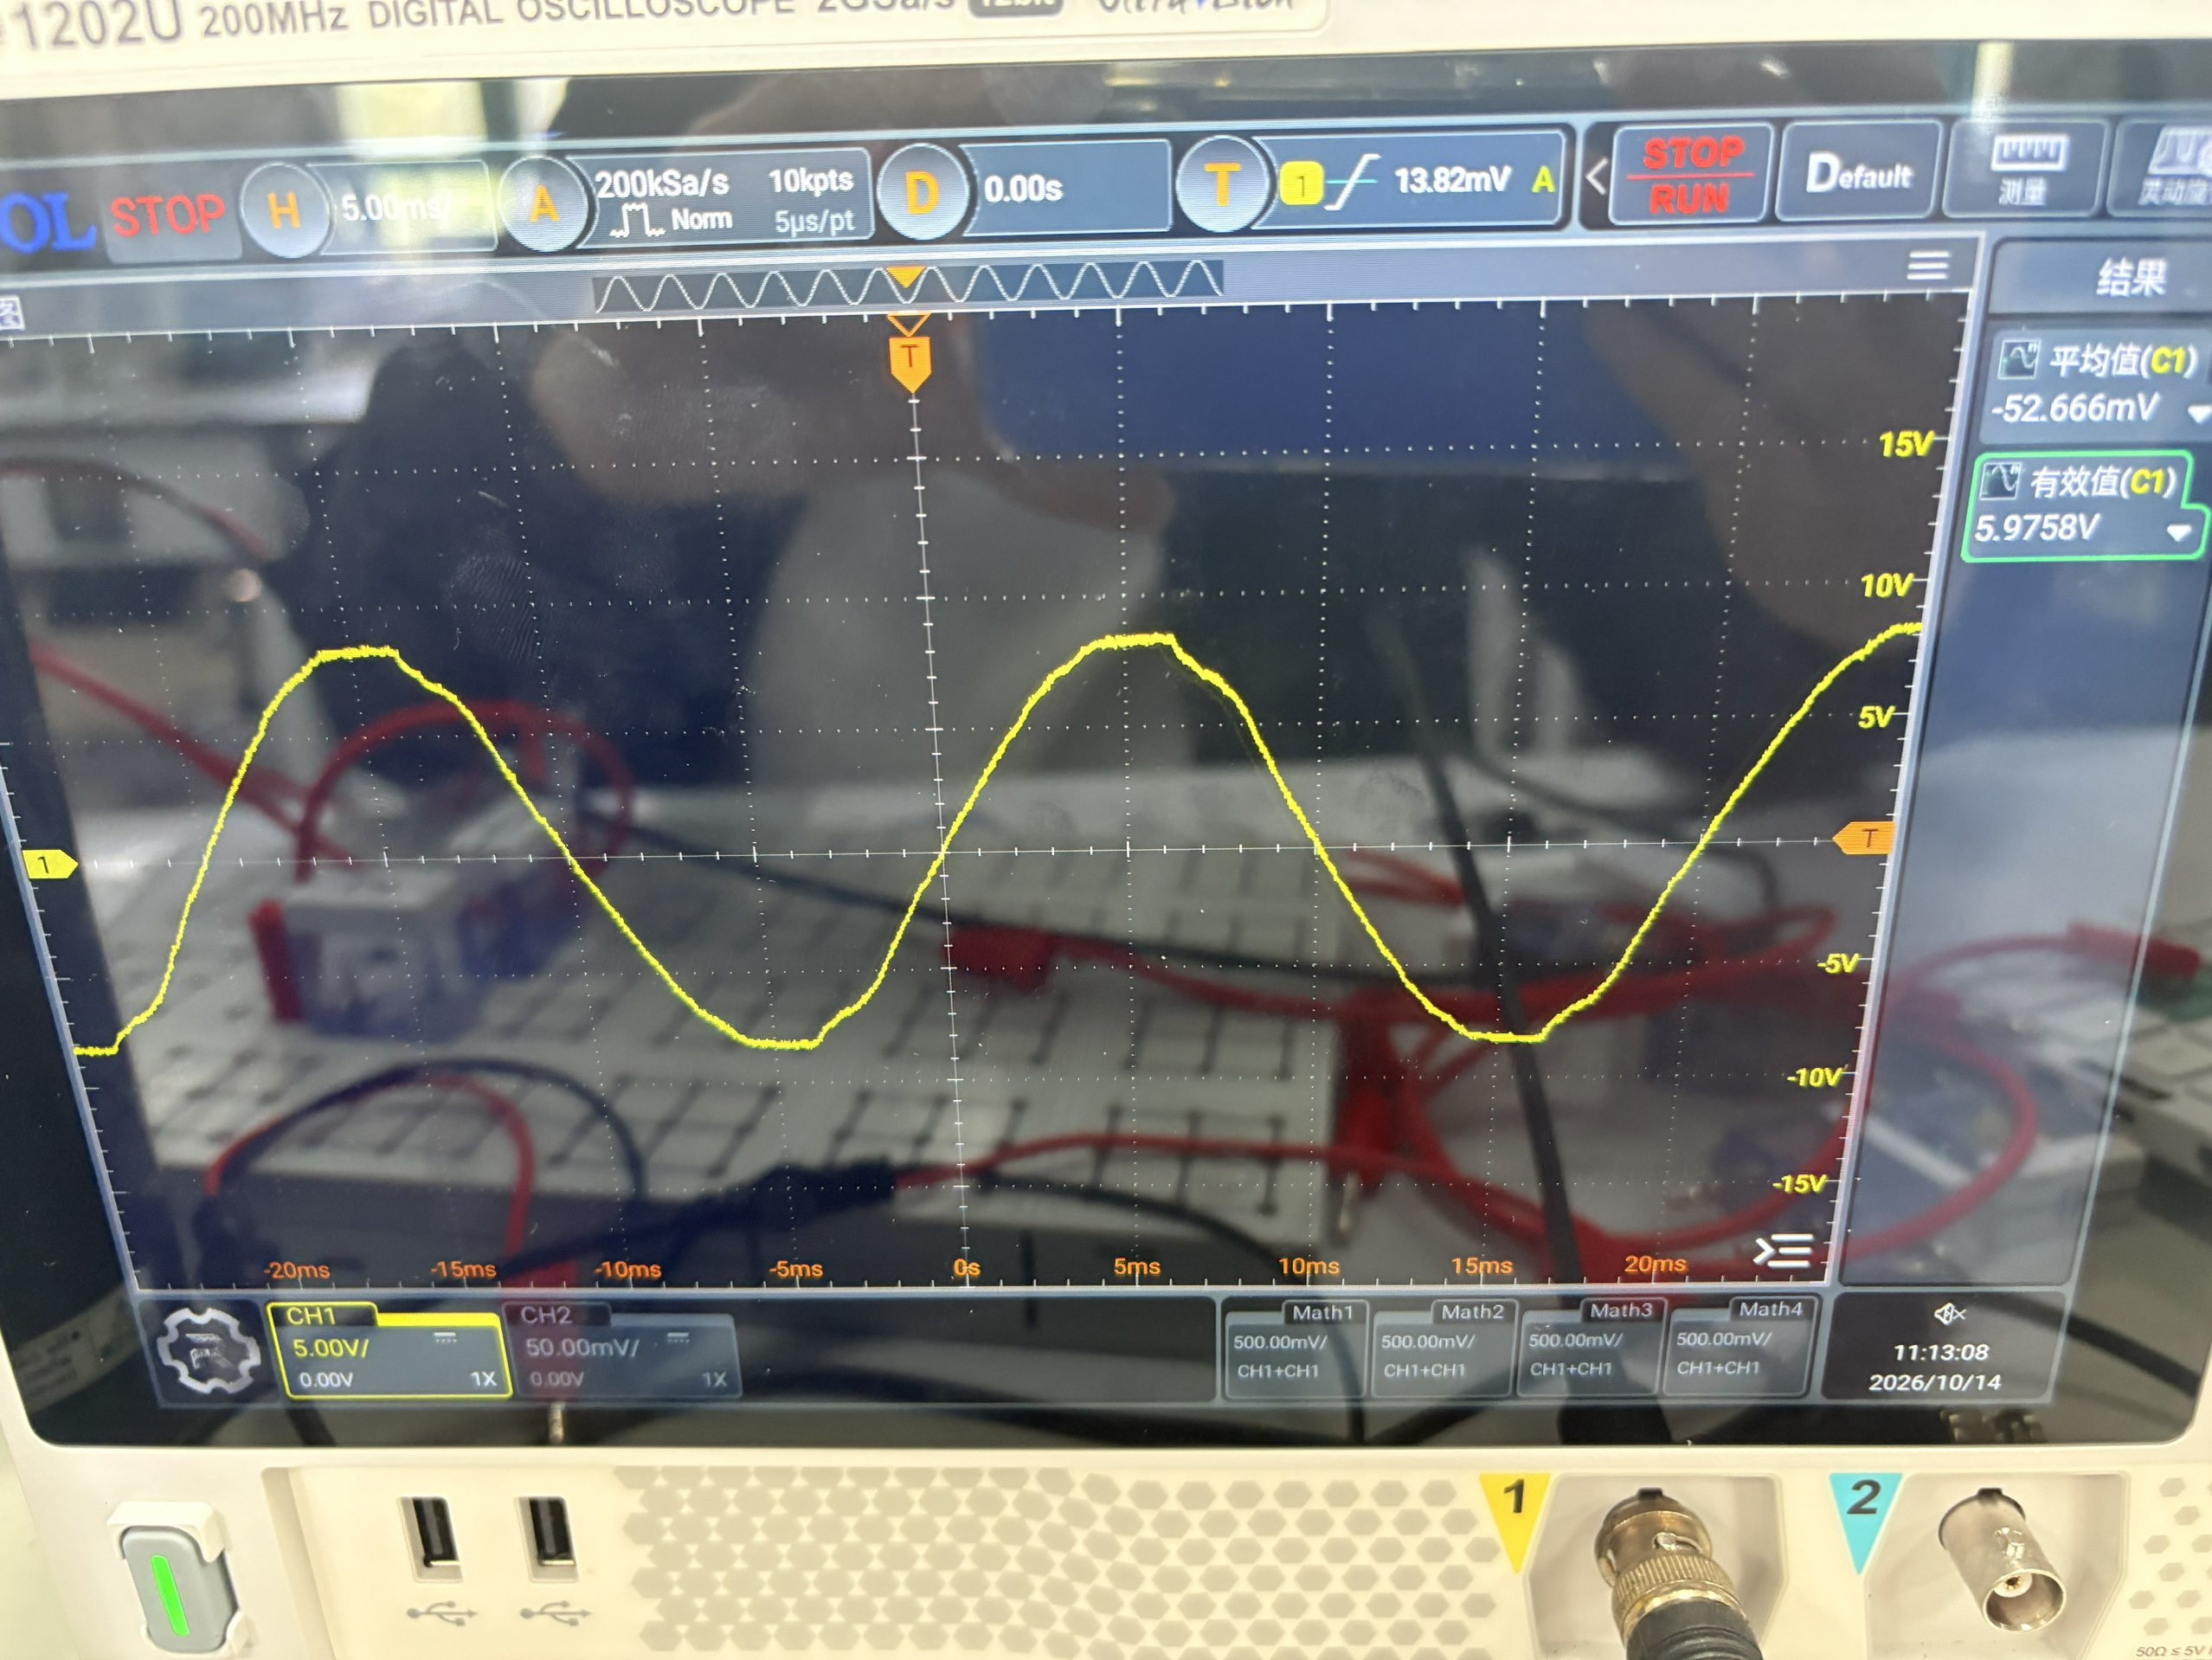
\includegraphics[width=0.1\textwidth]{figures/图18.png} & 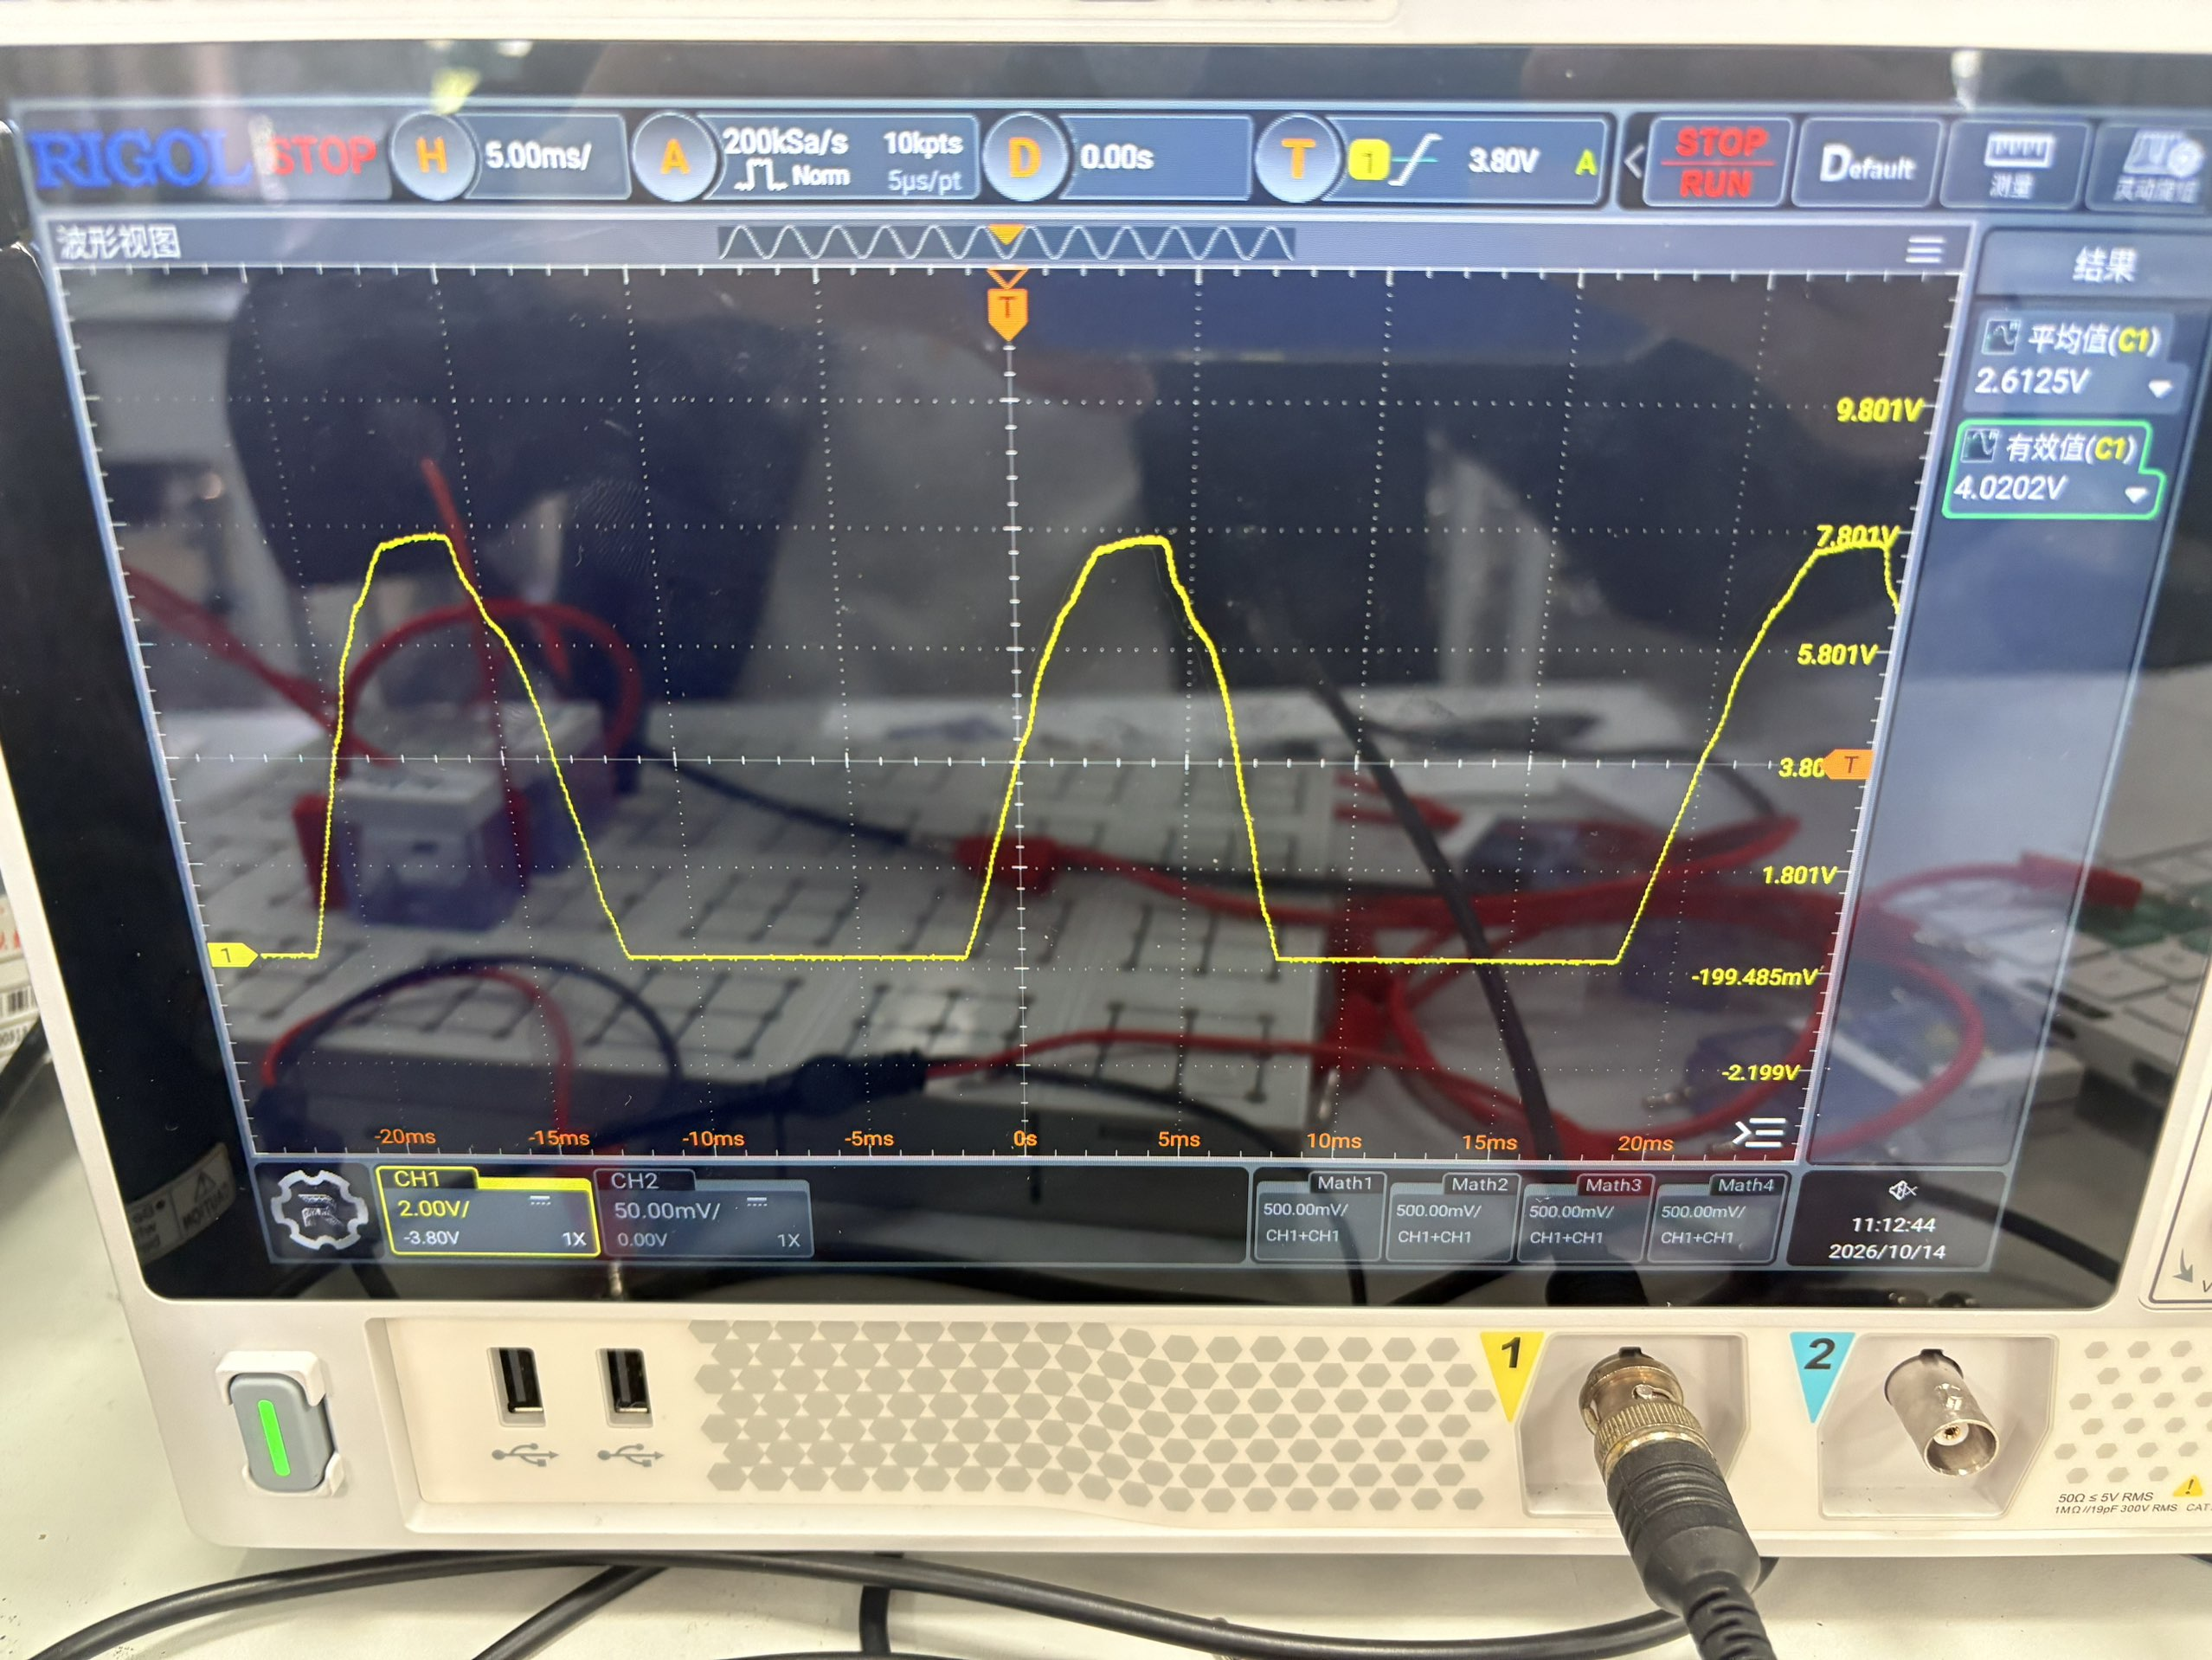
\includegraphics[width=0.1\textwidth]{figures/图19.png} \\
        单相全波整流电路 & 4.7114 & 5.9770 & 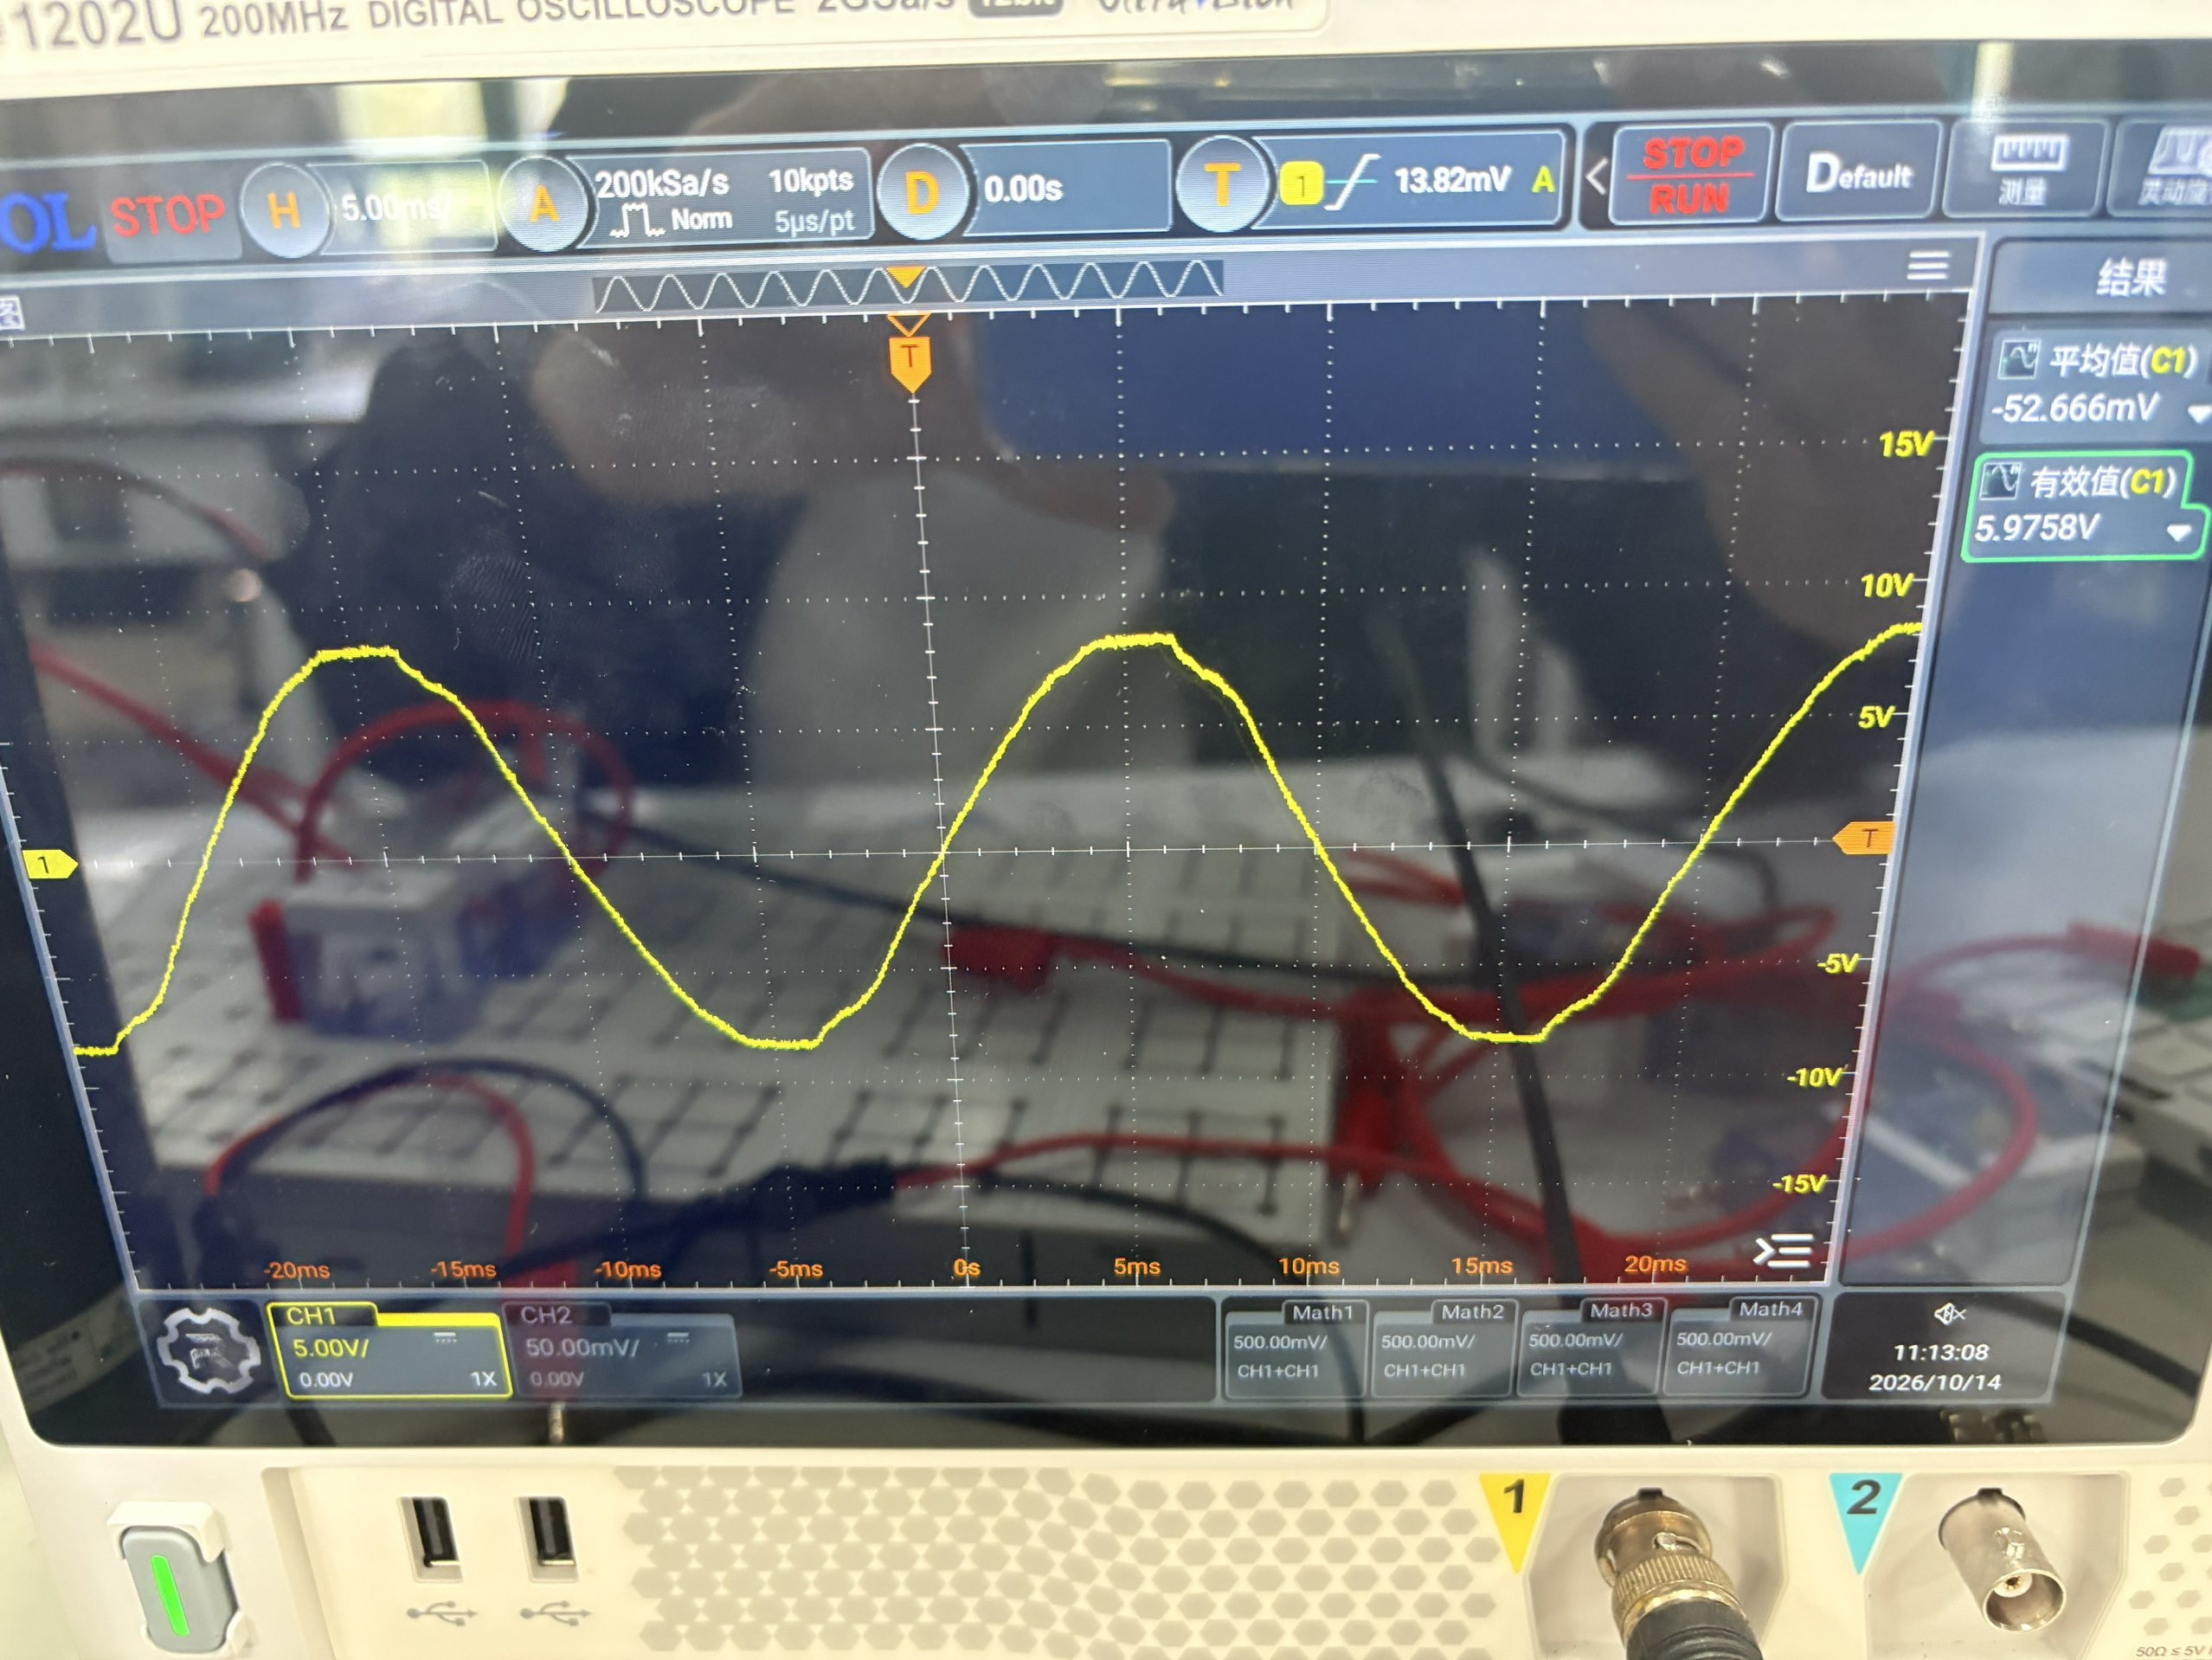
\includegraphics[width=0.1\textwidth]{figures/图18.png} & 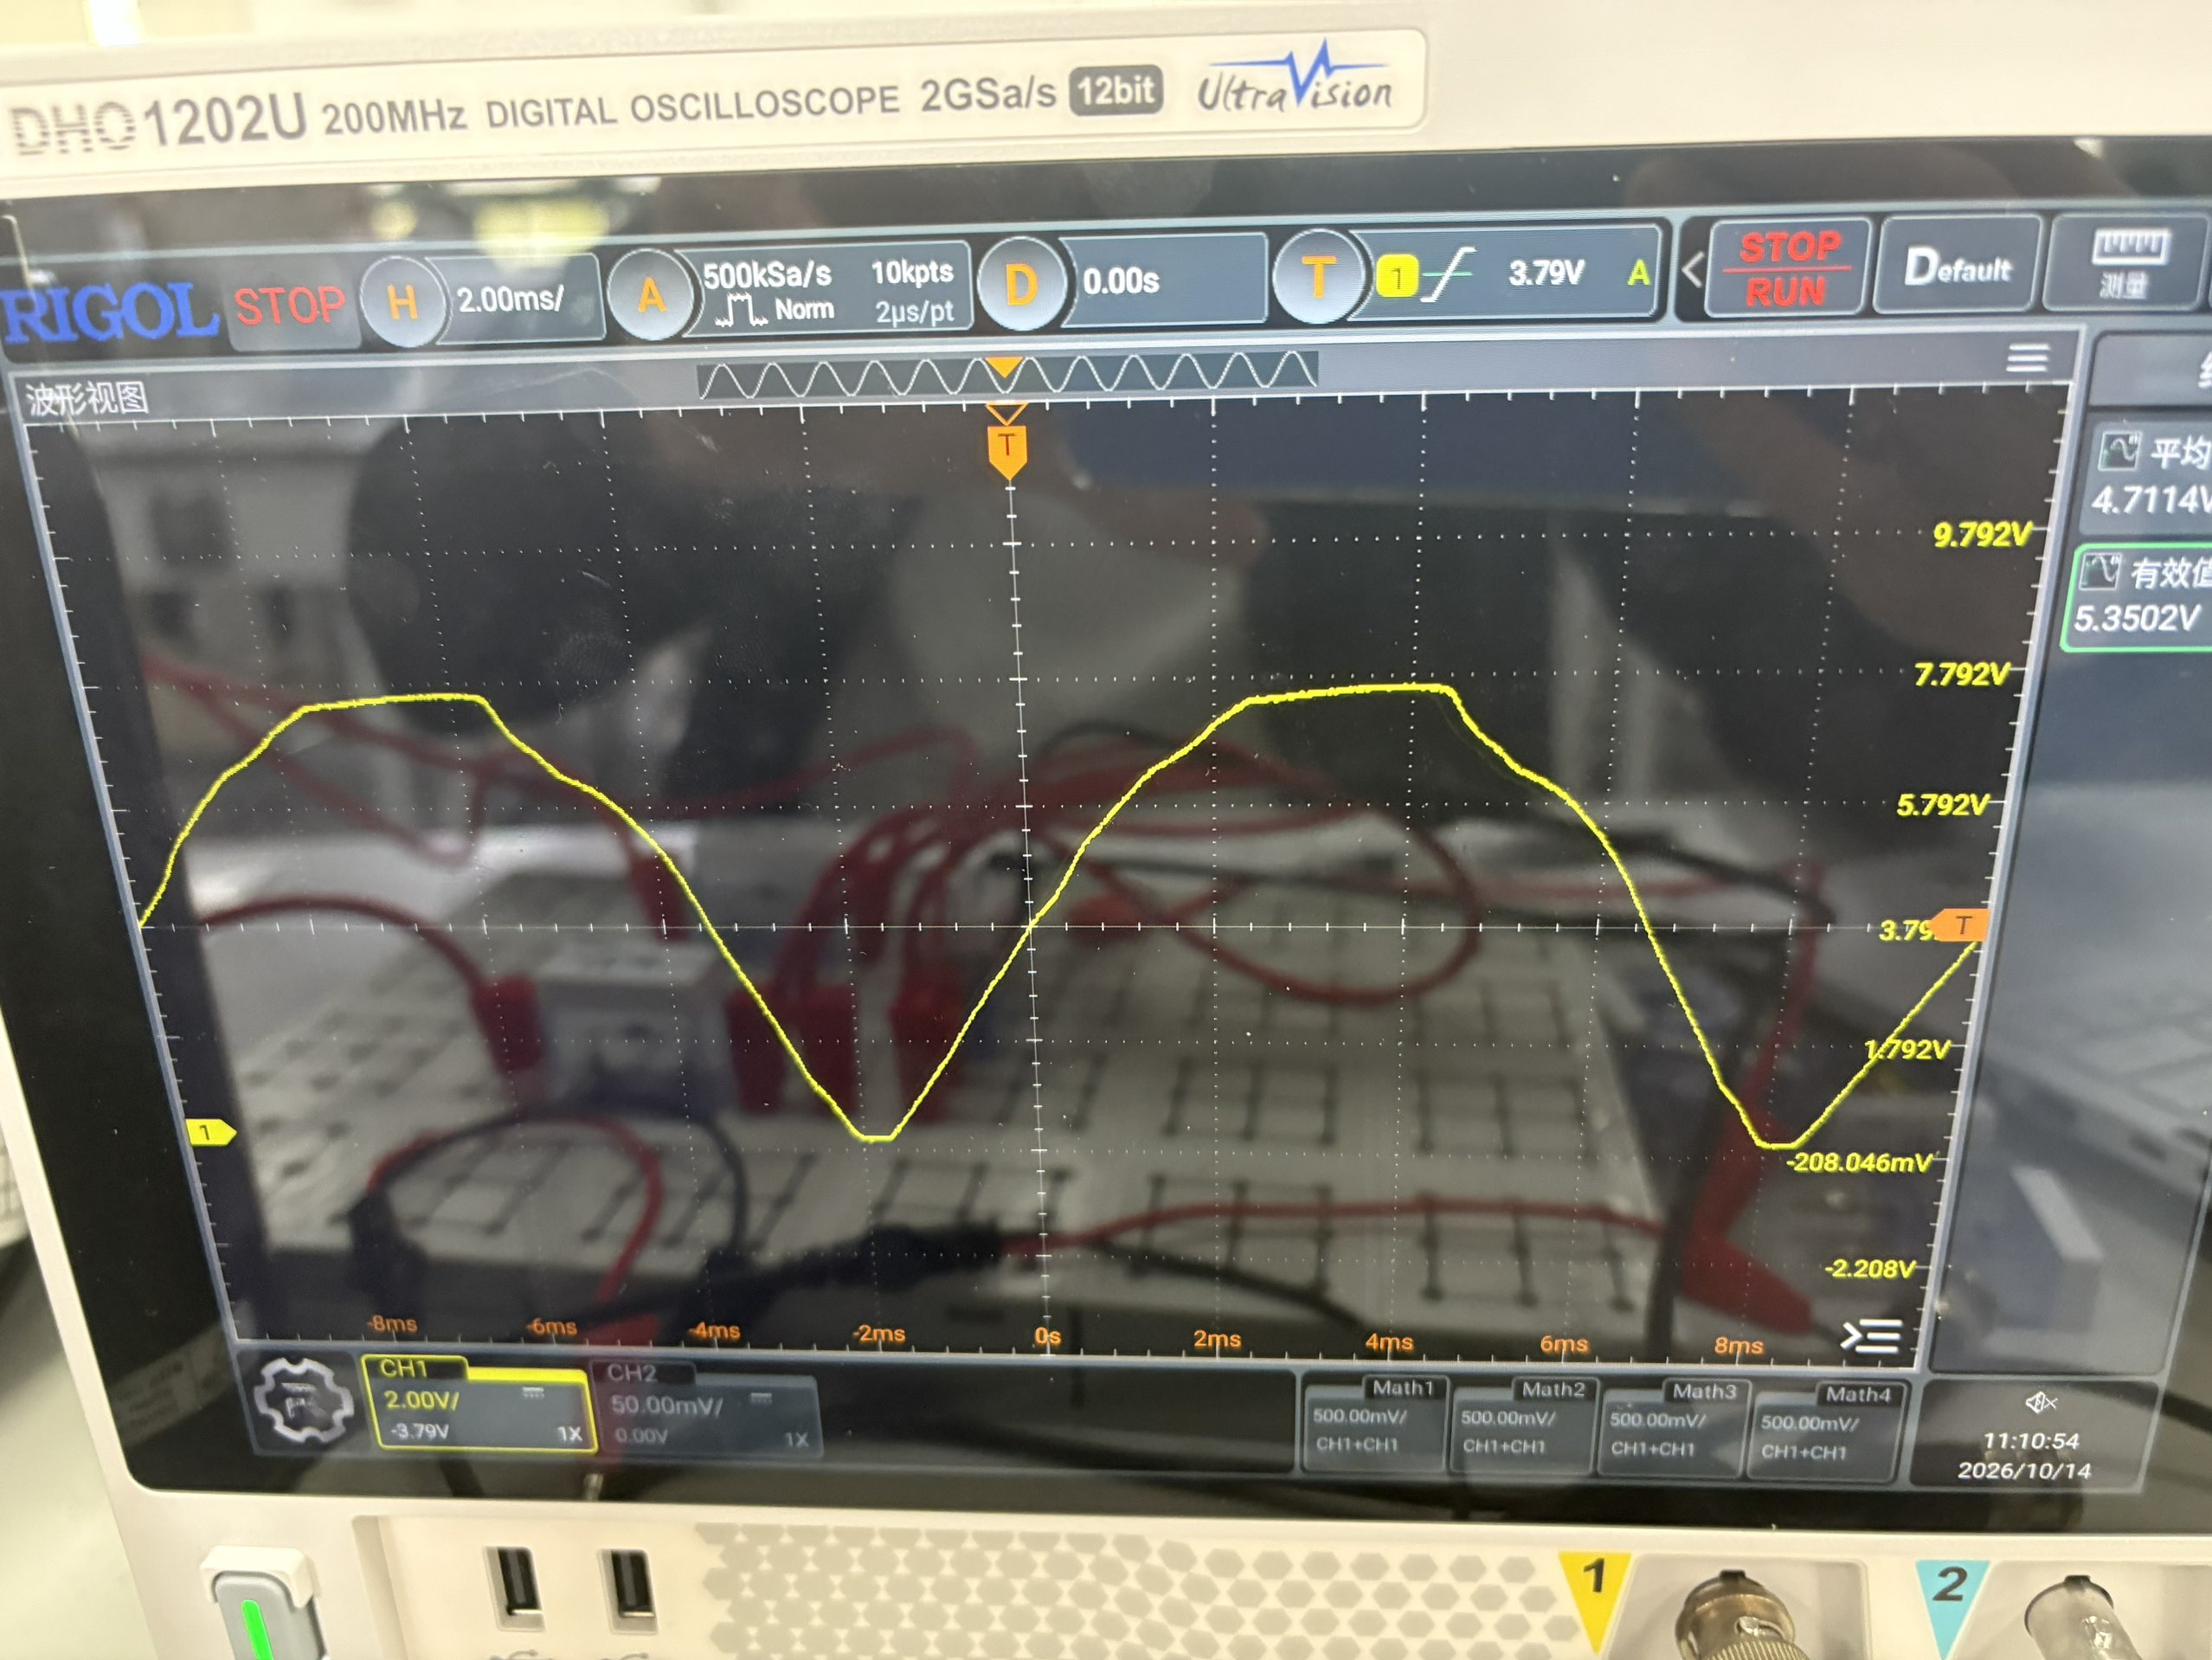
\includegraphics[width=0.1\textwidth]{figures/图20.png} \\
        单相桥式整流电路 & 4.1134 & 5.9578 & 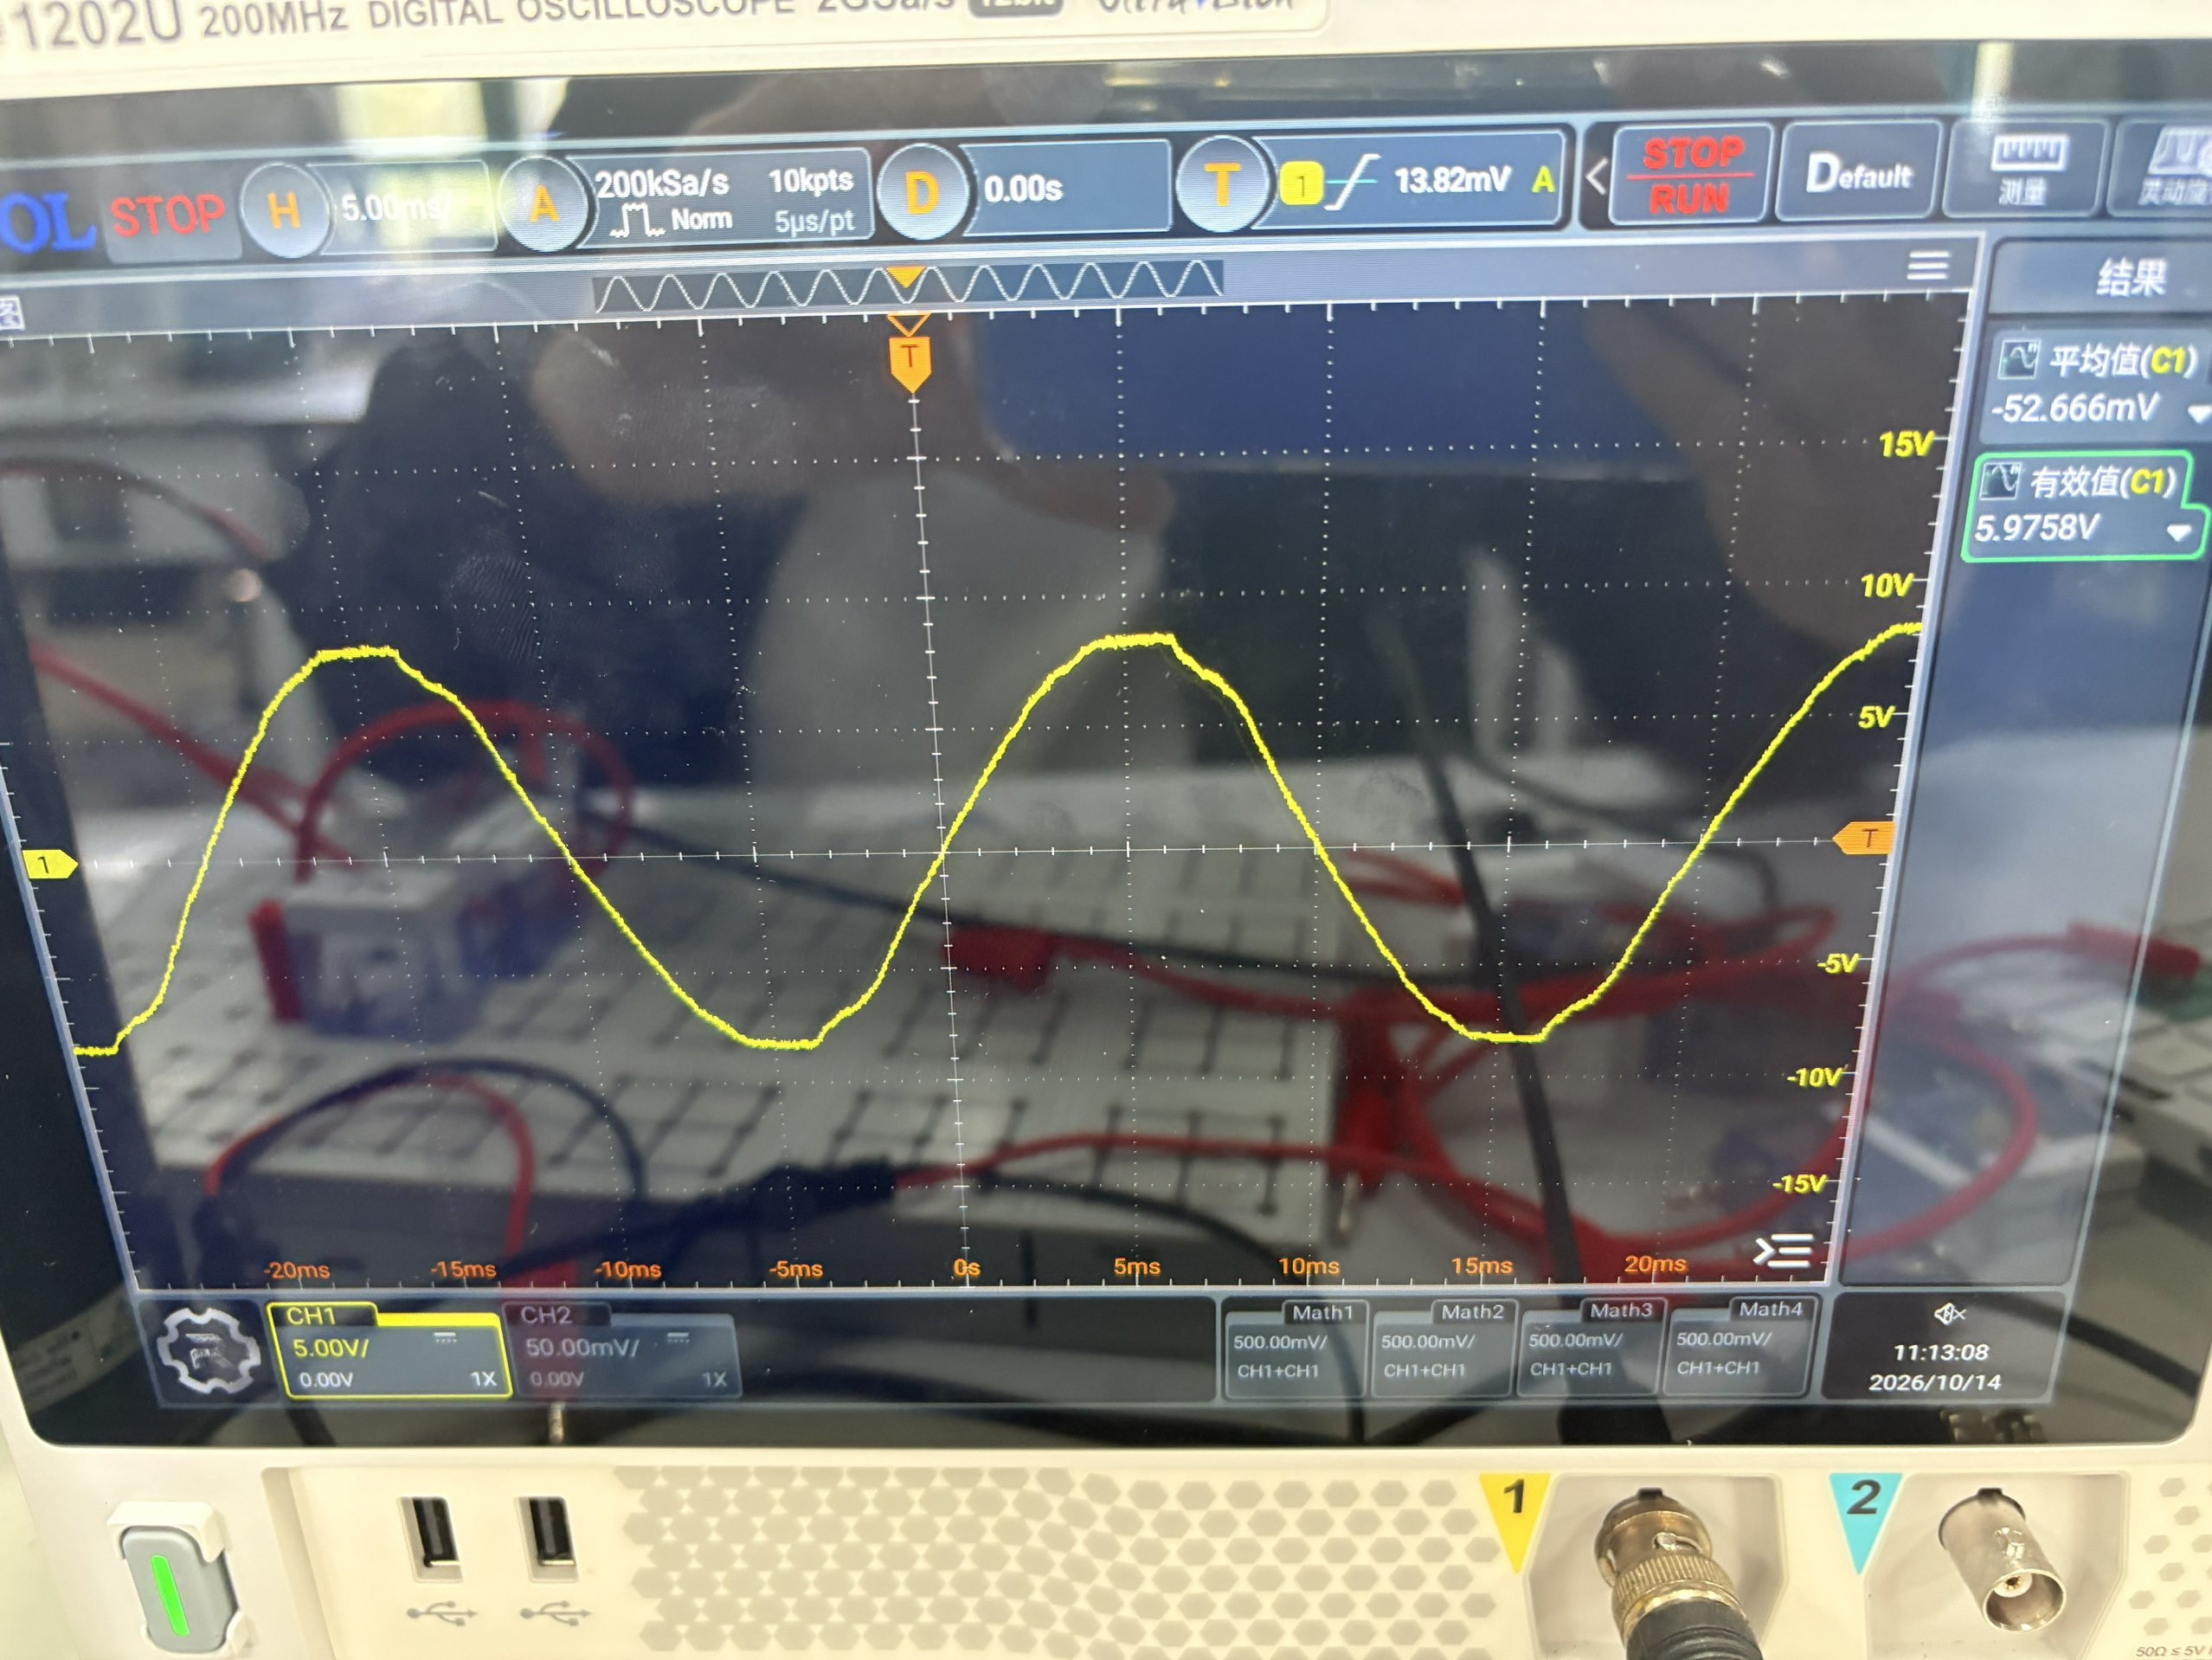
\includegraphics[width=0.1\textwidth]{figures/图18.png} & 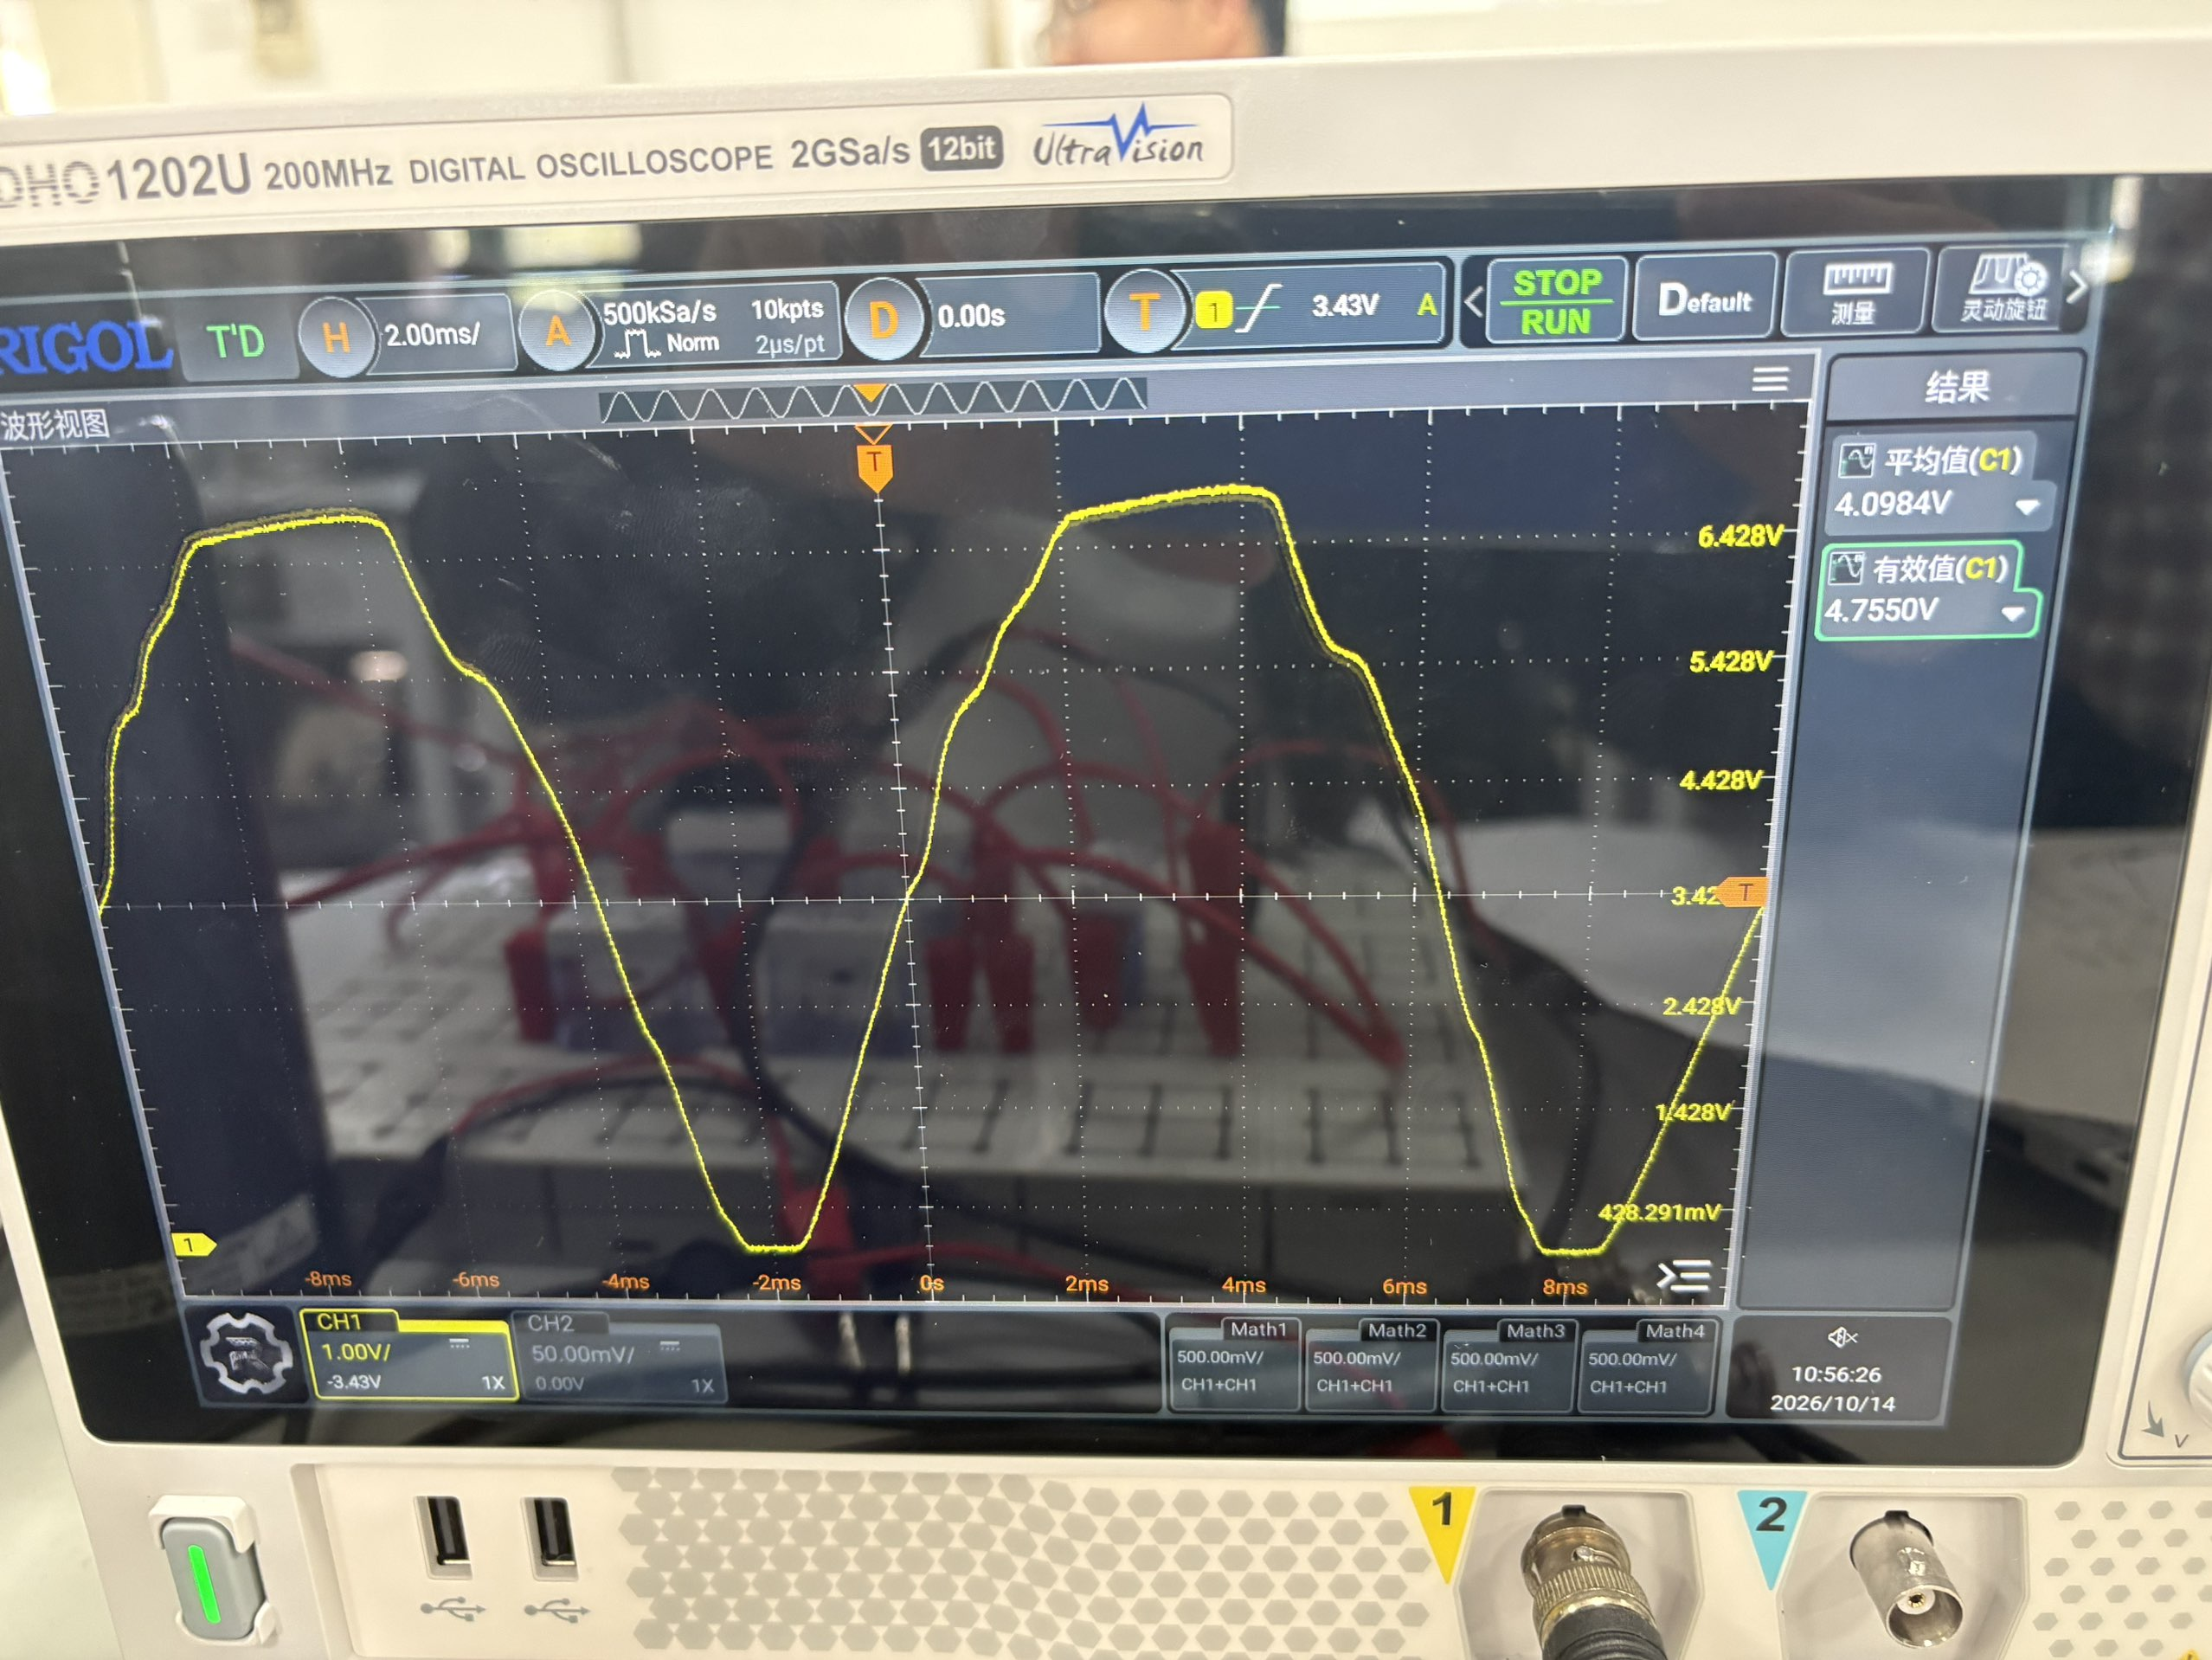
\includegraphics[width=0.1\textwidth]{figures/图21.png} \\
        \bottomrule
      \end{tabular}
    \end{table}

    忽略二极管的正向导通压降，三种整流电路输出平均电压的理论值分别为：
    \[
    \begin{aligned}
      \text{半波：}\quad \overline{U}_{0,\text{理论}} &= 0.45U_2 \\
      \text{全波：}\quad \overline{U}_{0,\text{理论}} &= 0.90U_2 \\
      \text{桥式：}\quad \overline{U}_{0,\text{理论}} &= 0.90U_2
    \end{aligned}
    \]

    以理论值为参照，实测平均电压的相对误差计算公式为：
    \[
      E=\frac{\left|\overline{U}_{0,\text{理论}}-\overline{U}_0\right|}
      {\overline{U}_{0,\text{理论}}}\times100\%
    \]
    
    然后将测量数据代入计算相对误差。

    \begin{samepage}
    （1）半波：
    \[
    \begin{aligned}
      \overline{U}_{0,\text{理论}}
        &=0.45\times5.9776=2.6899\,\mathrm{V} \\
      E_{\text{半波}}
        &=\frac{|2.6899-2.6125|}{2.6899}\times100\%=2.88\%
    \end{aligned}
    \]
    \end{samepage}

    \begin{samepage}
    （2）全波：
    \[
    \begin{aligned}
      \overline{U}_{0,\text{理论}}
        &=0.90\times5.9770=5.3793\,\mathrm{V} \\
      E_{\text{全波}}
        &=\frac{|5.3793-4.7114|}{5.3793}\times100\%=12.4\%
    \end{aligned}
    \]
    \end{samepage}

    \begin{samepage}
    （3）桥式：
    \[
    \begin{aligned}
      \overline{U}_{0,\text{理论}}
        &=0.90\times5.9578=5.3620\,\mathrm{V} \\
      E_{\text{桥式}}
        &=\frac{|5.3620-4.1134|}{5.3620}\times100\%=23.3\%
    \end{aligned}
    \]
    \end{samepage}

    完成上述三种整流电路测量后, 分别将47$\mu$F和470$\mu$F的电容接入桥式整流电路, 得到滤波后的波形图像如下:
    \begin{figure}[H]
      \centering
      \begin{minipage}[c]{0.45\textwidth}
        \centering
        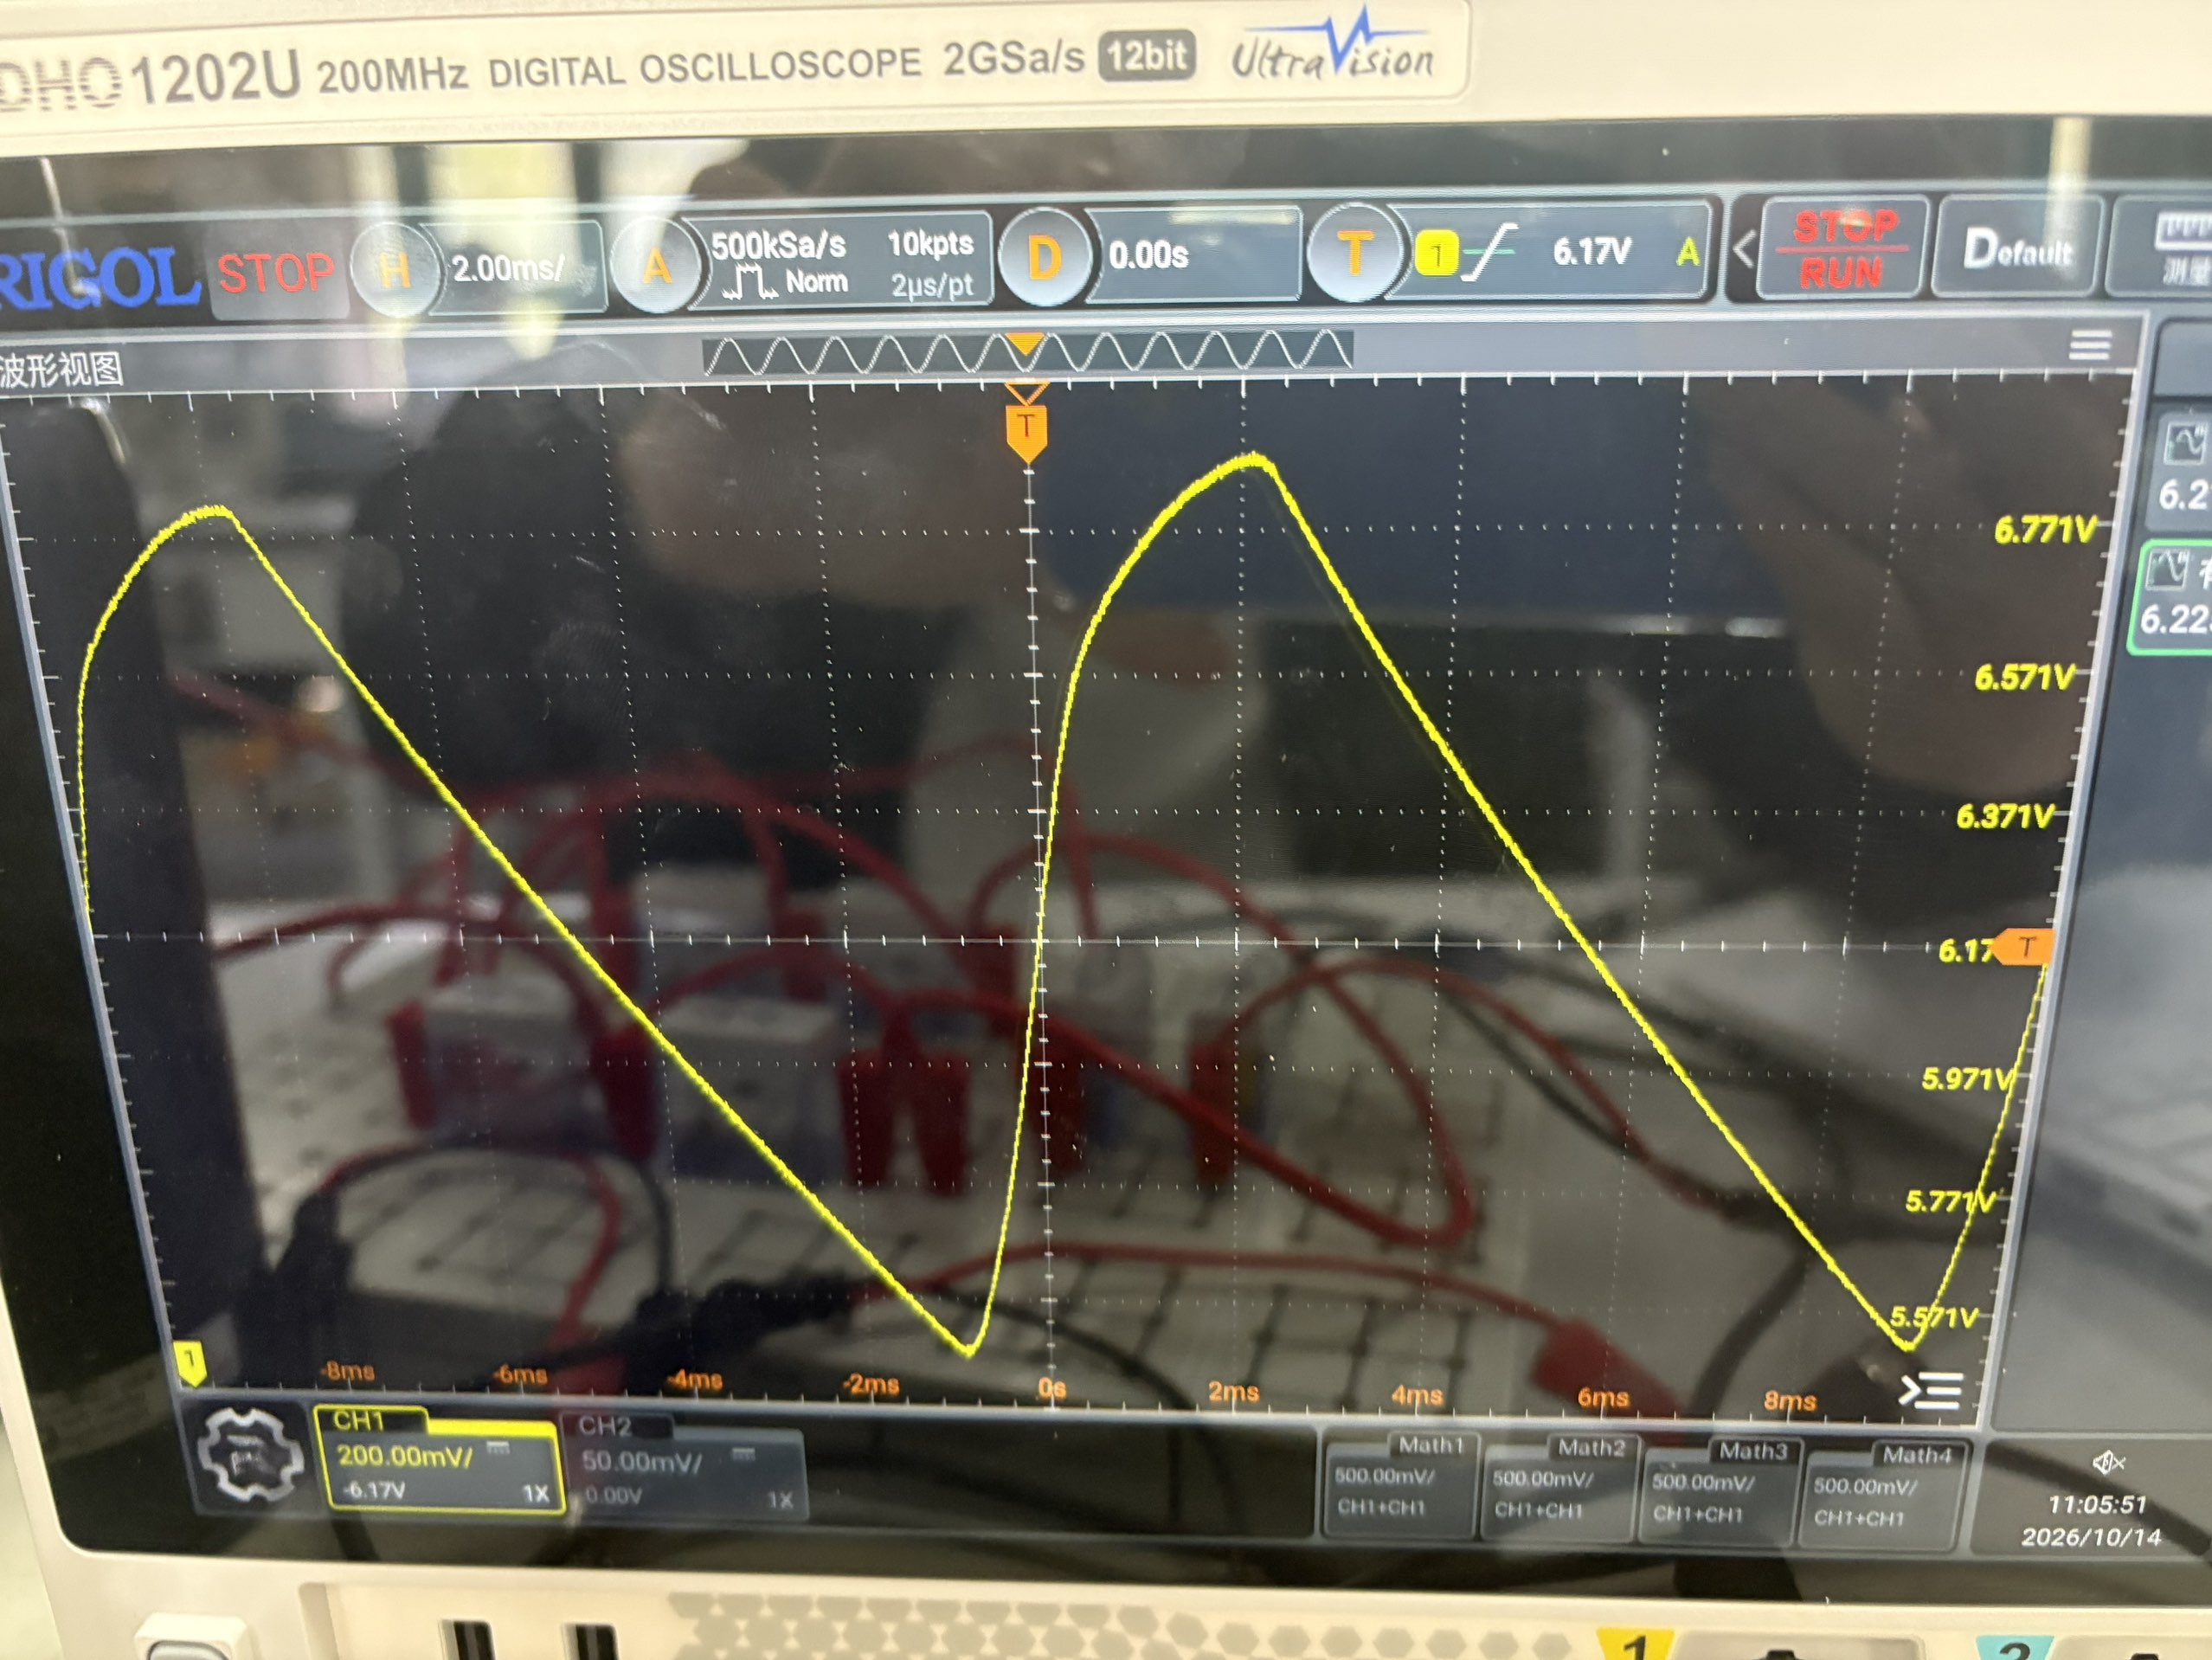
\includegraphics[width=0.8\textwidth]{figures/图22.png}
        \caption{接入47$\mu$F电容后的波形图}
      \end{minipage}
      \begin{minipage}[c]{0.45\textwidth}
        \centering
        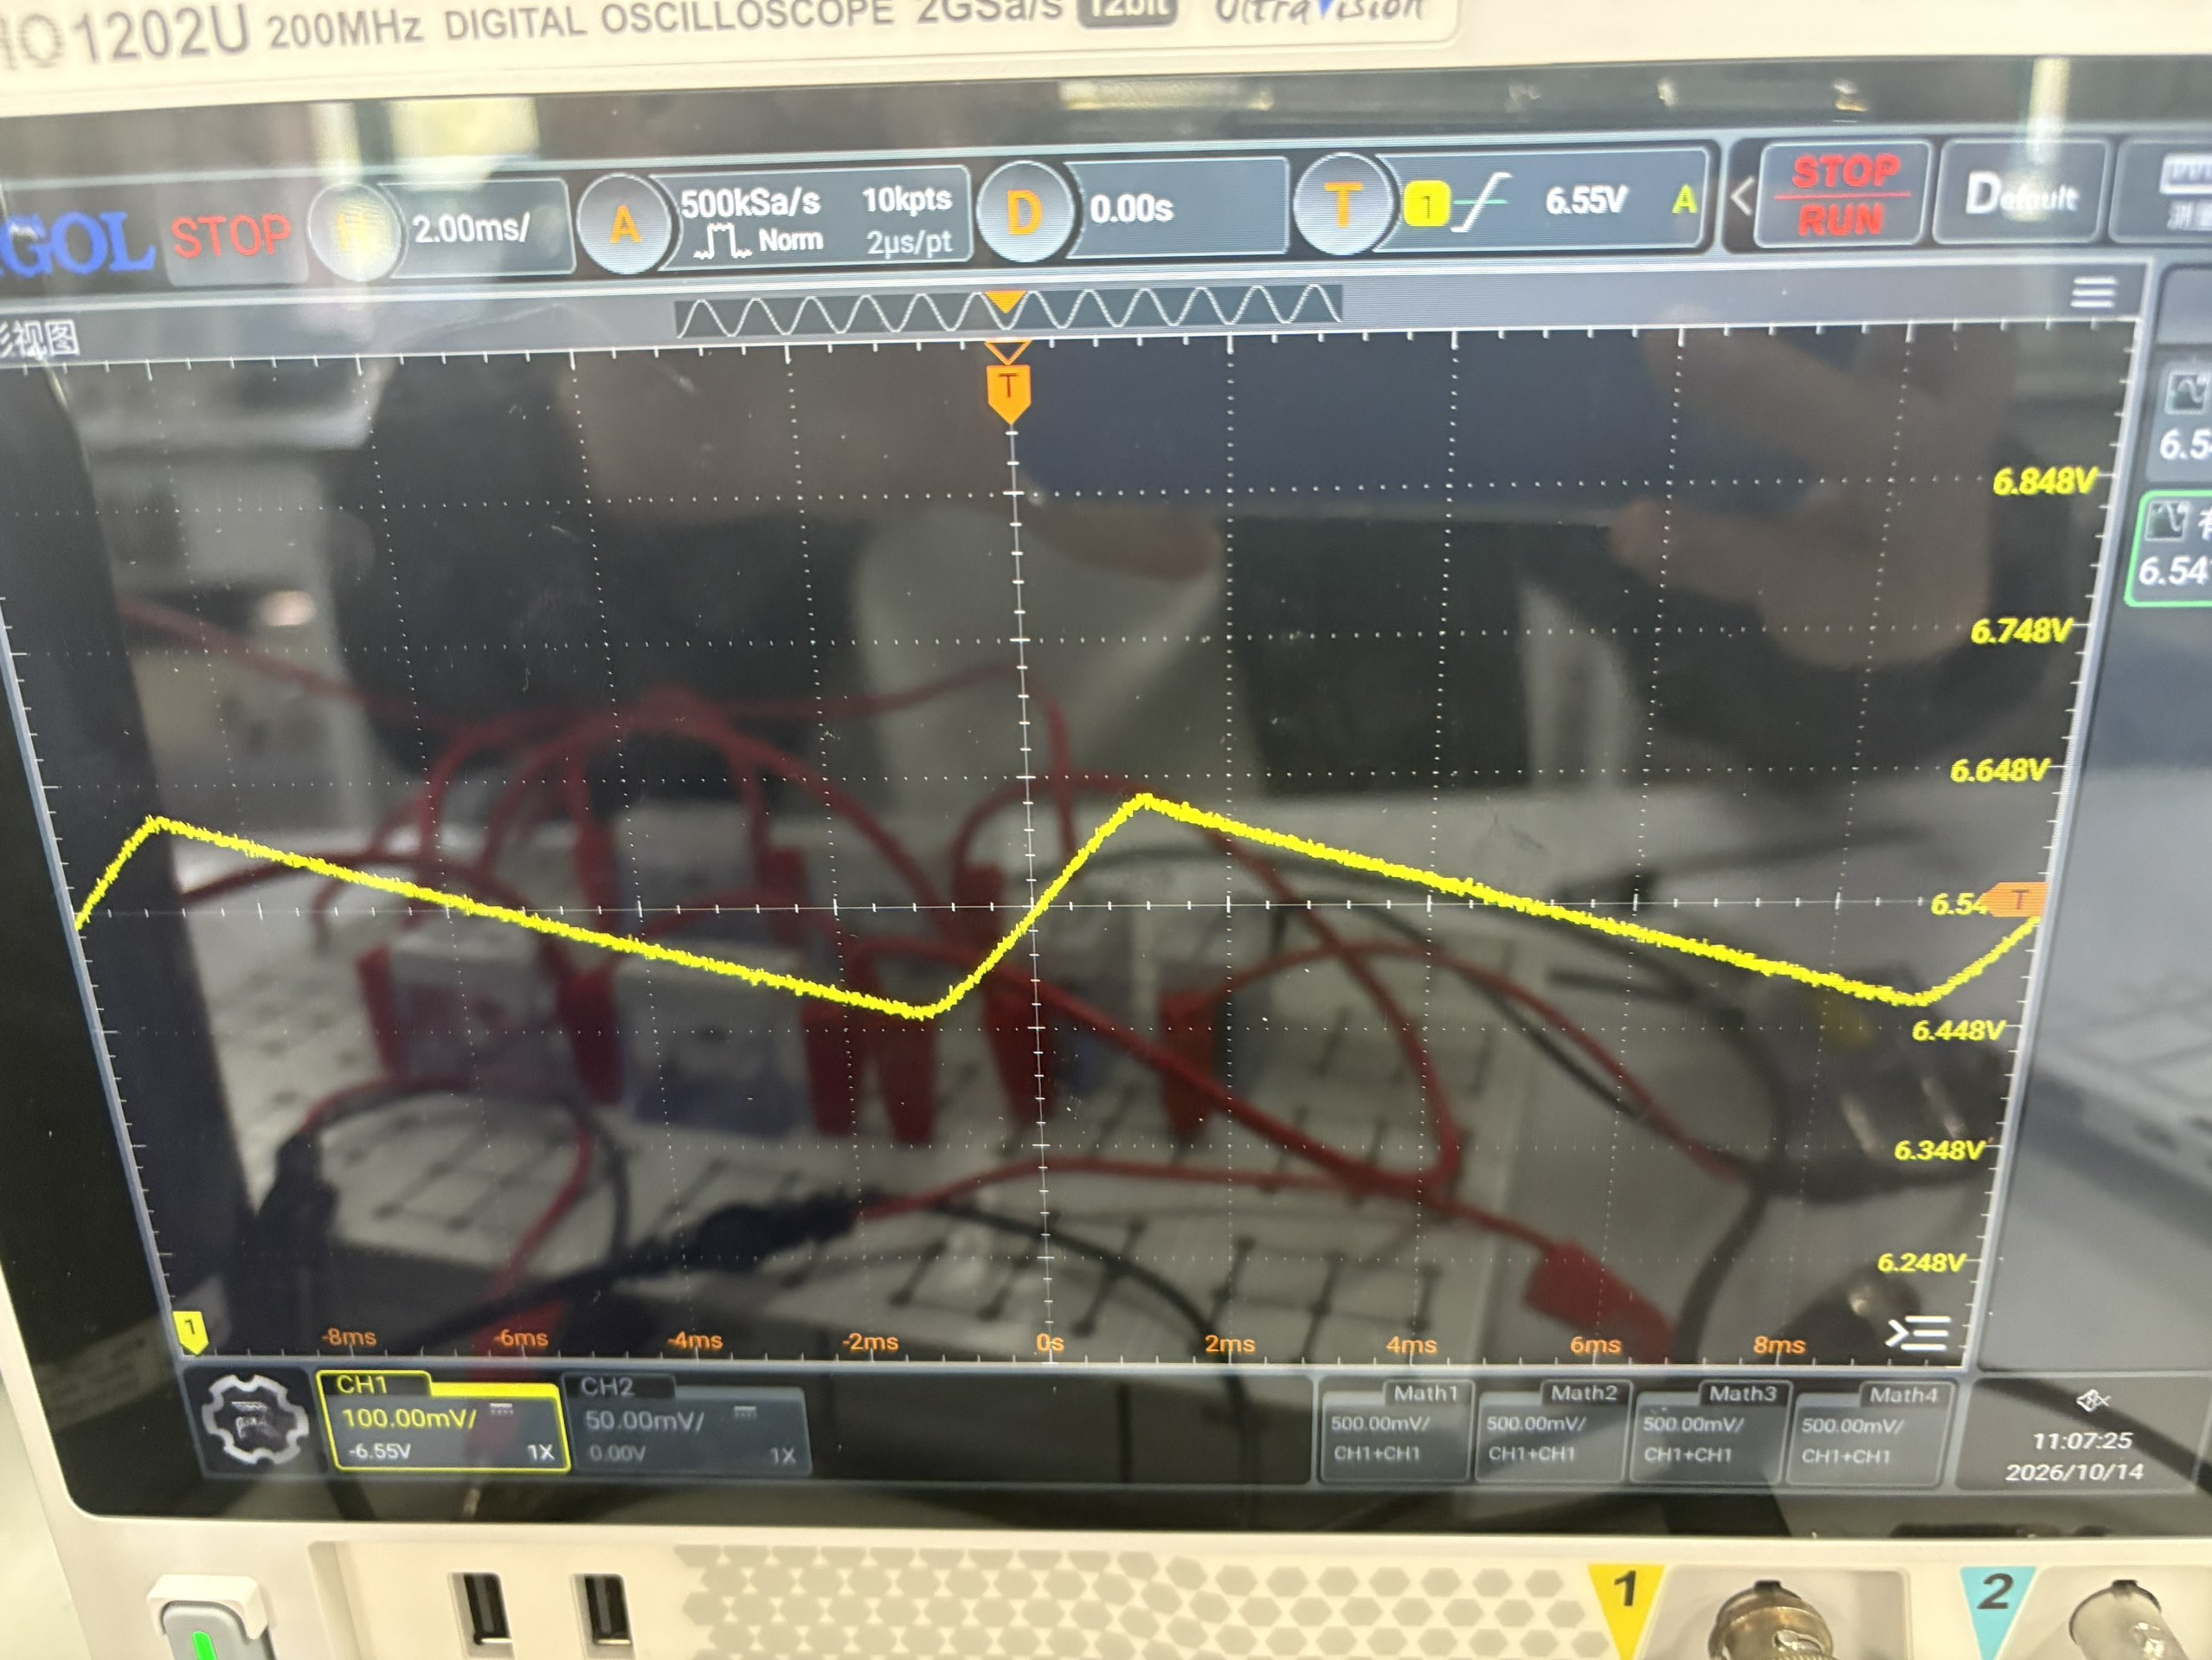
\includegraphics[width=0.8\textwidth]{figures/图23.png}
        \caption{接入470$\mu$F电容后的波形图}
      \end{minipage}
    \end{figure}

    由两幅示波器图像可见，电容取值对滤波效果有明显影响。
    接入$47\,\mu\mathrm{F}$电容时，输出电压在相邻峰值之间下降较明显，仍有较大的周期性脉动，
    说明电容在两次充电之间放电较快，滤波效果有限。
    接入$470\,\mu\mathrm{F}$电容后，相比$47\,\mu\mathrm{F}$时，电压在相邻峰值之间的下降幅度和纹波均明显减小，输出电压更加平稳，已取得较好的滤波效果。
    比较时应注意两图的电压量程不同，不能只根据波形在屏幕上的高度判断纹波大小。

    在负载电阻$R_L$一定时，电容放电的时间常数为
    \[
      \tau=R_L C
    \]
    
    电容越大，时间常数越大，电容通过负载放电越慢，输出电压在两次充电之间的下降越小，因而纹波减小。
    本实验中电容由$47\,\mu\mathrm{F}$增至$470\,\mu\mathrm{F}$，在其他条件相同时，时间常数增为原来的10倍，
    与图中滤波效果改善的趋势一致。

  \subsection{误差分析（10分）}
  
    \subsubsection{示波器的使用}
    示波器的使用实验中，误差主要来源于以下几个方面：
    \begin{enumerate}
      \item 二极管导通电压测量中，波形线宽、信号噪声、电压刻度分辨率以及光标位置的选择都会影响读数。
      \item RC电路相位差测量中，周期和时间差的读取精度、光标定位误差、两路波形触发不同步以及波形噪声都会造成测量结果偏差。
      \item 李萨如图形测频中，图形稳定性、边缘清晰程度、交点数判断以及信号频率的微小变化会影响测量结果。
    \end{enumerate}
    
    此外，示波器本身的测量分辨率、校准误差和操作人员的读数差异也会对实验结果产生影响。

    \subsubsection{组装整流器}
    我们已经得到了如下表所示的三种整流电路的相对误差。

    \begin{table}[H]
      \centering
      \caption{三种整流电路相对误差}
      \begin{tabular}{cccc}
        \toprule
        整流电路类型 & $\overline{U}_{0,\text{理论}}/\mathrm{V}$ & ${\overline{U}_{0}}/\mathrm{V}$ & $E/\%$ \\
        \midrule
        单相半波整流电路 & 2.6899 & 2.6125 & 2.88 \\
        单相全波整流电路 & 5.3793 & 4.7114 & 12.4 \\
        单相桥式整流电路 & 5.3620 & 4.1134 & 23.3 \\
        \bottomrule
      \end{tabular}
    \end{table}

    接下来分析误差的可能来源。

    （1）系统误差：理论计算将二极管视为理想元件，忽略了正向导通压降和导通后的动态电阻，
    因而理论输出平均电压偏高，这是本实验相对误差的主要来源。
    半波使用一只二极管；全波由两只二极管组成，在正、负半周期各有一只导通；桥式由四只二极管组成，每个半周期有两只串联导通，因而导通回路中的压降损失更大。
    信号源内阻、导线及接触电阻还会在导通时产生附加压降；示波器的测量精度、探头倍率和耦合设置也会影响电压读数。

    （2）环境因素与元件参数差异：二极管的正向压降随电流和温度变化，同型号器件的特性也不完全一致；
    电阻、电容的实际值与标称值存在偏差，电容的漏电和等效串联电阻也会影响滤波效果。
    此外，信号波动、噪声和触发不稳定会降低读数稳定性，自动测量的取样时窗未覆盖完整周期时，也可能使平均值出现偏差。

    （3）结果分析：半波、全波、桥式的相对误差分别为$2.88\%$、$12.4\%$和$23.3\%$，且实测平均电压均低于理论值。
    其中桥式偏差最大，与两只二极管串联导通造成较大压降的影响一致。
    半波的相对误差较小，并不代表其输出脉动最小或整流效果最好；
    全波和桥式仍能利用交流电的两个半周期，而电容滤波能够进一步减小输出脉动。

\section{实验探讨与思考题（10分）}

  \subsection{实验探讨}

    通过示波器的使用，我熟悉了如何通过触发、时基和电压量程等不同方式来调节示波器，认识到稳定清晰的波形是准确测量的前提。
    两种测量方法，自动测量与光标法可相互比较核对；
    观察李萨如图形时，需耐心微调频率，待图形稳定后再进行读数。

    组装整流器时，我加深了对半波、全波、桥式及电容滤波的理解。
    接线前应核对二极管方向和电容极性，再通过波形检查电路。
    实验中，大电容的滤波效果更明显；实测值与理论值存在差异时，应结合导通压降和负载分析，不能只凭偏差大小否定测量。

  \subsection{思考题}

    \subsubsection{示波器自动和光标法测量电压的误差分别主要来自哪里？}

    自动测量：自然因素主要包括信号噪声、温度和电源波动，以及仪器精度、采样分辨率的限制；
    人为因素主要是探头倍率、耦合方式或量程设置不当，使自动识别和计算产生偏差。

    光标法：自然因素主要是噪声和波形波动使峰值位置不易确定，以及屏幕分辨率的限制；
    人为因素主要是光标定位不准、读数偏差及量程选择不当，其中光标定位的影响较明显。

    \subsubsection{总结不同整流电路和不同滤波电路的利弊。}

    （1）整流电路：半波用一只二极管，结构简单、成本低，但只利用半个周期，平均电压低、脉动大。
    全波用两只二极管，每个半周期一只导通，平均电压较高、脉动较小，但需中心抽头变压器，反向耐压要求较高。
    桥式用四只二极管，无需中心抽头，变压器利用率高，但每个半周期两只串联导通，压降较大。

    \begin{samepage}
    （2）滤波电路：电容滤波简单，增大电容可减小脉动，但充电冲击电流增大。
    RC滤波结构简单、成本低，适合小电流负载，但电阻有压降和功率损耗；
    LC滤波效果较好、损耗较小，适合大电流负载，但体积大、成本高。\par
    \end{samepage}

    \subsubsection{整流和滤波的目的分别是什么？如果本实验计算的相对误差偏大，可能的主要误差来源是什么？}

    整流的目的是利用二极管的单向导电性，将交流电转换为单向的脉动直流电，但输出电压仍存在周期性变化。滤波的目的是减小整流输出中的交流分量和纹波；本实验利用电容的充放电作用，使输出电压更加平稳，改善直流供电质量。
    
    相对误差偏大的主要原因是理论计算忽略了二极管的正向导通压降，使理论输出电压偏高。
    半波和全波每个半周期均有一只二极管导通，桥式则有两只串联导通，压降影响更大。
    输入电压较低时，这种影响尤其明显；信号源内阻、负载效应和读数偏差也会引入误差。

\vspace*{\fill} % 使下面内容在页面底部显示
\noindent
\begin{minipage}{\textwidth}
  注意事项：

  \begingroup
    \setlength{\leftskip}{2em} % 1--4整体向右缩进两个汉字宽度
    1. 用PDF格式上传“实验报告”，文件名：学生姓名+学号+实验名称+周次。

    2. “实验报告”必须递交在“学在浙大”本课程内对应实验项目的“作业”模块内。

    3. “实验报告”成绩必须在“浙江大学物理实验教学中心网站”-“选课系统”内查询。

    4. 教学评价必须在“浙江大学物理实验教学中心网站”-“选课系统”内进行，学生必须进行教学评价，才能看到实验报告成绩，教学评价须在本次实验结束之后3天内进行。\par
  \endgroup

  \begin{center}
    {\CJKfontspec[AutoFakeBold=2.5]{SimSun}\bfseries 浙江大学物理实验教学中心制}
  \end{center}
\end{minipage}

\end{document}
